%%%  کلاس AUTthesis، نسخه آبان 1397
%%%   دانشگاه صنعتی امیرکبیر                 http://www.aut.ac.ir
%%%  تالار گفتگوی پارسی‌لاتک،       http://forum.parsilatex.com
%%%   آپدیت شده در آبان 95
%%%   پشتیبانی و راهنمایی          badali_farhad@yahoo.com
%%%
%%%   بازبینی و اصلاح شده در آبان ماه 1397
%%%  Tested via TeXstudio in TeXlive 2014-2018.
%%%

%-----------------------------------------------------------------------------------------------------
%        روش اجرا.: 2 بار F1 ، 2 بار  F11(به منظور تولید مراجع) ، دوبار Ctrl+Alt+I (به منظور تولید نمایه) و دو بار F1 -------> مشاهده Pdf
%%%%%%%%%%%%%%%%%%%%%%%%%%%%%%%%%%%%%%%%%%%%%%%%%%%%%%
%   TeXstudio as your IDE
%%  برای compile در TeXstudio تنها کافی است منوی Options->Configure TeXstudio را زده و در پنجره Configure TeXstudio در بخش Build گزینه Default Compiler را به XeLaTeX تغییر دهید. سند شما به راحتی compile خواهد شد.
%   F1 & F5 : Build & view
%   F6      : Compile
%   F7      : View
%   --------------
%%%%%%%%%%%%%%%%%%%%%%%%%%%%%%%%%%%%%%%%%%%%%%%%%%%%%%
%        اگر قصد نوشتن رساله دکتری را دارید، در خط زیر به جای msc،
%      کلمه phd را قرار دهید. کلیه تنظیمات لازم، به طور خودکار، اعمال می‌شود.
%%% !TEX TS-program = XeLaTeX
\documentclass[oneside,bsc,12pt]{AUTthesis}
%       فایل commands.tex را حتماً به دقت مطالعه کنید؛ چون دستورات مربوط به فراخوانی بسته زی‌پرشین 
%       و دیگر بسته‌ها و ... در این فایل قرار دارد و بهتر است که با نحوه استفاده از آنها آشنا شوید. توجه شود برای نسخه نهایی پایان‌نامه حتماً hyperref را 
%        غیرفعال کنید.


% در این فایل، دستورها و تنظیمات مورد نیاز، آورده شده است.
%-------------------------------------------------------------------------------------------------------------------
% در ورژن جدید زی‌پرشین برای تایپ متن‌های ریاضی، این سه بسته، حتماً باید فراخوانی شود.
\usepackage{amsthm,amssymb,amsmath,amsfonts}
% بسته‌ای برای تنطیم حاشیه‌های بالا، پایین، چپ و راست صفحه
\usepackage[top=30mm, bottom=30mm, left=25mm, right=30mm]{geometry}
% بسته‌‌ای برای ظاهر شدن شکل‌ها و تصاویر متن
\usepackage{graphicx}
\usepackage{wrapfig}
\usepackage{caption}
\usepackage{subcaption}
\usepackage{color}
%بسته‌ای برای تنظیم فاصله عمودی خط‌های متن
\usepackage{setspace}
\usepackage{titletoc}
\usepackage{tocloft}
%با فعال کردن بسته زیر فوت‌نوت‌ها در هر صفحه ریست می‌شوند. حالت پیش‌فرض آن ریست شدن در هر فصل می‌باشد.
%\usepackage[perpage]{footmisc}
\usepackage{enumitem}
\usepackage{caption}
%\usepackage{titlesec}

% دستوراتی که شما تعریف می‌کنید:
\newcommand{\pcb}{{\lr{PCB}} }
\newcommand{\pcbf}{{پی‌سی‌بی} }

%تصاویر در فولدر زیر قرار دارند:
%\graphicspath{ {./images/Khanch/} }
\graphicspath{ {./images/} }

% بسته‌ و دستوراتی برای ایجاد لینک‌های رنگی با امکان جهش
\usepackage[pagebackref=false,colorlinks,linkcolor=blue,citecolor=red]{hyperref}
\usepackage[nameinlink]{cleveref}%capitalize,,noabbrev
 \AtBeginDocument{%
    \crefname{equation}{برابری}{equations}%
    \crefname{chapter}{فصل}{chapters}%
    \crefname{section}{بخش}{sections}%
    \crefname{appendix}{پیوست}{appendices}%
    \crefname{enumi}{مورد}{items}%
    \crefname{footnote}{زیرنویس}{footnotes}%
    \crefname{figure}{شکل}{figures}%
    \crefname{table}{جدول}{tables}%
    \crefname{theorem}{قضیه}{theorems}%
    \crefname{lemma}{لم}{lemmas}%
    \crefname{corollary}{نتیجه}{corollaries}%
    \crefname{proposition}{گزاره}{propositions}%
    \crefname{definition}{تعریف}{definitions}%
    \crefname{result}{نتیجه}{results}%
    \crefname{example}{مثال}{examples}%
    \crefname{remark}{نکته}{remarks}%
    \crefname{note}{یادداشت}{notes}%
}
% چنانچه قصد پرینت گرفتن نوشته خود را دارید، خط بالا را غیرفعال و  از دستور زیر استفاده کنید چون در صورت استفاده از دستور زیر‌‌، 
% لینک‌ها به رنگ سیاه ظاهر خواهند شد که برای پرینت گرفتن، مناسب‌تر است
%\usepackage[pagebackref=false]{hyperref}
% بسته‌ لازم برای تنظیم سربرگ‌ها
\usepackage{fancyhdr}
% بسته‌ای برای ظاهر شدن «مراجع»  در فهرست مطالب
\usepackage[nottoc]{tocbibind}
% دستورات مربوط به ایجاد نمایه
\usepackage{makeidx,multicol}
\setlength{\columnsep}{1.5cm}

\usepackage[bottom]{footmisc}
\usepackage{float}
%%%%%%%%%%%%%%%%%%%%%%%%%%
\usepackage{verbatim}
\makeindex
\usepackage{sectsty}
% فراخوانی بسته زی‌پرشین و تعریف قلم فارسی و انگلیسی
\usepackage{xepersian}%[extrafootnotefeatures]
\SepMark{-}
%حتماً از تک لایو 2014 استفاده کنید.
\settextfont[Scale=1.2]{B Nazanin.ttf}
\setlatintextfont{Times New Roman.ttf}
\renewcommand{\labelitemi}{$\bullet$}
%%%%%%%%%%%%%%%%%%%%%%%%%%
% چنانچه می‌خواهید اعداد در فرمول‌ها، انگلیسی باشد، خط زیر را غیرفعال کنید.
%در غیر اینصورت حتماً فونت PGaramond را نصب کنید.
\setdigitfont[Scale=1.1]{Yas.ttf}%%Yas
%%%%%%%%%%%%%%%%%%%%%%%%%%
% تعریف قلم‌های فارسی اضافی برای استفاده در بعضی از قسمت‌های متن
\defpersianfont\nastaliq[Scale=2]{IranNastaliq.ttf}
\defpersianfont\chapternumber[Scale=3]{B Nazanin.ttf}

%\chapterfont{\centering}%
%%%%%%%%%%%%%%%%%%%%%%%%%%
% دستوری برای تغییر نام کلمه «اثبات» به «برهان»
\renewcommand\proofname{\textbf{برهان}}

% دستوری برای تغییر نام کلمه «کتاب‌نامه» به «منابع و مراجع«
\renewcommand{\bibname}{منابع و مراجع}


% Headings for every page of ToC, LoF and Lot
\setlength{\cftbeforetoctitleskip}{-1.2em}
\setlength{\cftbeforelottitleskip}{-1.2em}
\setlength{\cftbeforeloftitleskip}{-1.2em}
\setlength{\cftaftertoctitleskip}{-1em}
\setlength{\cftafterlottitleskip}{-1em}
\setlength{\cftafterloftitleskip}{-1em}
%%\makeatletter
%%%%\renewcommand{\l@chapter}{\@dottedtocline{1}{1em\bfseries}{1em}}
%%%%\renewcommand{\l@section}{\@dottedtocline{2}{2em}{2em}}
%%%%\renewcommand{\l@subsection}{\@dottedtocline{3}{3em}{3em}}
%%%%\renewcommand{\l@subsubsection}{\@dottedtocline{4}{4em}{4em}}
%%%%\makeatother


\newcommand\tocheading{\par عنوان\hfill صفحه \par}
\newcommand\lofheading{\hspace*{.5cm}\figurename\hfill صفحه \par}
\newcommand\lotheading{\hspace*{.5cm}\tablename\hfill صفحه \par}

\renewcommand{\cftchapleader}{\cftdotfill{\cftdotsep}}
\renewcommand{\cfttoctitlefont}{\hspace*{\fill}\LARGE\bfseries}%\Large
\renewcommand{\cftaftertoctitle}{\hspace*{\fill}}
\renewcommand{\cftlottitlefont}{\hspace*{\fill}\LARGE\bfseries}%\Large
\renewcommand{\cftafterlottitle}{\hspace*{\fill}}
\renewcommand{\cftloftitlefont}{\hspace*{\fill}\LARGE\bfseries}
\renewcommand{\cftafterloftitle}{\hspace*{\fill}}

%%%%%%%%%%%%%%%%%%%%%%%%%%
% تعریف و نحوه ظاهر شدن عنوان قضیه‌ها، تعریف‌ها، مثال‌ها و ...
%برای شماره گذاری سه تایی قضیه ها
\theoremstyle{definition}
\newtheorem{definition}{تعریف}[section]
\newtheorem{remark}[definition]{نکته}
\newtheorem{note}[definition]{یادداشت}
\newtheorem{example}[definition]{نمونه}
\newtheorem{question}[definition]{سوال}
\newtheorem{remember}[definition]{یاداوری}
\theoremstyle{theorem}
\newtheorem{theorem}[definition]{قضیه}
\newtheorem{lemma}[definition]{لم}
\newtheorem{proposition}[definition]{گزاره}
\newtheorem{corollary}[definition]{نتیجه}
%%%%%%%%%%%%%%%%%%%%%%%%
%%%%%%%%%%%%%%%%%%%
%%% برای شماره گذاری چهارتایی قضیه ها و ...
%%\newtheorem{definition1}[subsubsection]{تعریف}
%%\newtheorem{theorem1}[subsubsection]{قضیه}
%%\newtheorem{lemma1}[subsubsection]{لم}
%%\newtheorem{proposition1}[subsubsection]{گزاره}
%%\newtheorem{corollary1}[subsubsection]{نتیجه}
%%\newtheorem{remark1}[subsubsection]{نکته}
%%\newtheorem{example1}[subsubsection]{مثال}
%%\newtheorem{question1}[subsubsection]{سوال}

%%%%%%%%%%%%%%%%%%%%%%%%%%%%

% دستورهایی برای سفارشی کردن صفحات اول فصل‌ها
\makeatletter
\newcommand\mycustomraggedright{%
 \if@RTL\raggedleft%
 \else\raggedright%
 \fi}
\def\@makechapterhead#1{%
\thispagestyle{style1}
\vspace*{20\p@}%
{\parindent \z@ \mycustomraggedright
\ifnum \c@secnumdepth >\m@ne
\if@mainmatter

\bfseries{\Huge \@chapapp}\small\space {\chapternumber\thechapter}
\par\nobreak
\vskip 0\p@
\fi
\fi
\interlinepenalty\@M 
\Huge \bfseries #1\par\nobreak
\vskip 120\p@

}

%\thispagestyle{empty}
\newpage}
\bidi@patchcmd{\@makechapterhead}{\thechapter}{\tartibi{chapter}}{}{}
\bidi@patchcmd{\chaptermark}{\thechapter}{\tartibi{chapter}}{}{}
\makeatother

\pagestyle{fancy}
\renewcommand{\chaptermark}[1]{\markboth{\chaptername~\tartibi{chapter}: #1}{}}

\fancypagestyle{style1}{
\fancyhf{} 
\fancyfoot[c]{\thepage}
\fancyhead[R]{\leftmark}%
\renewcommand{\headrulewidth}{1.2pt}
}


\fancypagestyle{style2}{
\fancyhf{}
\fancyhead[R]{چکیده}
\fancyfoot[C]{\thepage{}}
\renewcommand{\headrulewidth}{1.2pt}
}

\fancypagestyle{style3}{%
  \fancyhf{}%
  \fancyhead[R]{فهرست نمادها}
  \fancyfoot[C]{\thepage}%
  \renewcommand{\headrulewidth}{1.2pt}%
}

\fancypagestyle{style4}{%
  \fancyhf{}%
  \fancyhead[R]{فهرست جداول}
  \fancyfoot[C]{\thepage}%
  \renewcommand{\headrulewidth}{1.2pt}%
}

\fancypagestyle{style5}{%
  \fancyhf{}%
  \fancyhead[R]{فهرست اشکال}
  \fancyfoot[C]{\thepage}%
  \renewcommand{\headrulewidth}{1.2pt}%
}

\fancypagestyle{style6}{%
  \fancyhf{}%
  \fancyhead[R]{فهرست مطالب}
  \fancyfoot[C]{\thepage}%
  \renewcommand{\headrulewidth}{1.2pt}%
}

\fancypagestyle{style7}{%
  \fancyhf{}%
  \fancyhead[R]{نمایه}
  \fancyfoot[C]{\thepage}%
  \renewcommand{\headrulewidth}{1.2pt}%
}

\fancypagestyle{style8}{%
  \fancyhf{}%
  \fancyhead[R]{منابع و مراجع}
  \fancyfoot[C]{\thepage}%
  \renewcommand{\headrulewidth}{1.2pt}%
}
\fancypagestyle{style9}{%
  \fancyhf{}%
  \fancyhead[R]{واژه‌نامه‌ی فارسی به انگلیسی}
  \fancyfoot[C]{\thepage}%
  \renewcommand{\headrulewidth}{1.2pt}%
}
%


%دستور حذف نام لیست تصاویر و لیست جداول از فهرست مطالب
\newcommand*{\BeginNoToc}{%
  \addtocontents{toc}{%
    \edef\protect\SavedTocDepth{\protect\the\protect\value{tocdepth}}%
  }%
  \addtocontents{toc}{%
    \protect\setcounter{tocdepth}{-10}%
  }%
}
\newcommand*{\EndNoToc}{%
  \addtocontents{toc}{%
    \protect\setcounter{tocdepth}{\protect\SavedTocDepth}%
  }%
}
\newcounter{savepage}
\renewcommand{\listfigurename}{فهرست اشکال}
\renewcommand{\listtablename}{فهرست جداول}
%\renewcommand\cftsecleader{\cftdotfill{\cftdotsep}}
%%%%%%%%%%%%%%%%%%%%%%%%%%%%%
%%%%%%%%%%%%%%%%%%%%%%%%%%%%

\begin{document}
\baselineskip=.75cm
\linespread{1.75}
%% -!TEX root = AUTthesis.tex
% در این فایل، عنوان پایان‌نامه، مشخصات خود، متن تقدیمی‌، ستایش، سپاس‌گزاری و چکیده پایان‌نامه را به فارسی، وارد کنید.
% توجه داشته باشید که جدول حاوی مشخصات پروژه/پایان‌نامه/رساله و همچنین، مشخصات داخل آن، به طور خودکار، درج می‌شود.
%%%%%%%%%%%%%%%%%%%%%%%%%%%%%%%%%%%%
% دانشکده، آموزشکده و یا پژوهشکده  خود را وارد کنید
\faculty{دانشکده مهندسی برق}
% گرایش و گروه آموزشی خود را وارد کنید
\department{گروه کنترل}
% عنوان پایان‌نامه را وارد کنید
\fatitle{طراحی  و ساخت ساعت مچی هوشمند
\\[.75 cm]
  با قابلیت تحلیل حرکات دست و پایش سلامت}
% نام استاد(ان) راهنما را وارد کنید
\firstsupervisor{دکتر محمداعظم خسروی}
\secondsupervisor{دکتر محمدباقر منهاج}
% نام استاد(دان) مشاور را وارد کنید. چنانچه استاد مشاور ندارید، دستور پایین را غیرفعال کنید.
%\firstadvisor{دکتر بهادر بخشی}
%\secondadvisor{استاد مشاور دوم}
% نام نویسنده را وارد کنید
\name{سلمان }
% نام خانوادگی نویسنده را وارد کنید
\surname{عامی مطلق}
%%%%%%%%%%%%%%%%%%%%%%%%%%%%%%%%%%
\thesisdate{مرداد 1401}

% چکیده پایان‌نامه را وارد کنید
\fa-abstract{
امروزه تجهیزاتی از قبیل تلفن‌همراه و ساعت‌های هوشمند جزء لاینفکی از زندگی مردم شده و استفاده‌ی رایجی دارند. از این رو بهبود تعاملات انسان و سامانه‌های هوشمند می‌تواند برگ برنده‌ای برای این صنعت باشد. یکی از جنبه‌های این تعامل، برقراری ارتباط بین ساعت هوشمند، تلفن‌همراه و پایش حرکات فیزیکی است. در این پروژه ابتدا یک ساعت هوشمند به صورت کامل طراحی شده است. این طراحی شامل سخت‌افزار، نرم‌افزار و طراحی مکانیکی بوده که از بستر بلوتوث برای برقراری ارتباط با تلفن‌همراه استفاده می‌کند. علاوه بر این، ساعت طراحی شده دارای حسگر شتاب،‌ حسگر سلامت (پالس‌اکسی‌متر)، بازر، موتور ایجاد لرزش، شارژر باتری لیتیومی، کلیدهای لمسی و صفحه‌ی نمایش است. به کمک حسگر شتاب و پردازش سیگنال آن، متغیرهای فضایی دست اندازه‌گیری شده و به کمک پیاده‌سازی دو فیلتر کالمن، اطلاعات حسگر فیلتر می‌شوند. این تشخیص حرکت برای مواردی مثل شمارش گام و روشن شدن صفحه نمایش در صورت بالا آمدن دست استفاده شده‌اند. برای پیاده‌سازی این فیلتر از تکنیک جاگذاری مقدار نهایی ضرایب استفاده شده است که باعث کاهش چشمگیر حجم محاسبات، کاهش حافظه‌ی مورد نیاز و افزایش سرعت اجرا است. پژوهش انجام شده‌ی پیش‌رو، نقطه‌ی پایانی برای این پروژه نیست و می‌توان ایده‌های زیادی برای پیشرفت و مسیر آینده‌ی این پروژه متصور شد. هدایت یک بازوی رباتیک بر اساس حرکت دست به کمک فناوری اینترنت اشیاء مثالی از این ایده‌ها است.
}


% کلمات کلیدی پایان‌نامه را وارد کنید
\keywords{ساعت هوشمند، فیلتر کالمن، ریزپردازنده، تلفن‌همراه هوشمند، دستگاه پوشیدنی}



\AUTtitle
%%%%%%%%%%%%%%%%%%%%%%%%%%%%%%%%%%
\vspace*{7cm}
\thispagestyle{empty}
\begin{center}

\includegraphics[height=5cm,width=12cm]{besm}
\end{center}
% تاییدیه دفاع
% \newpage
% \thispagestyle{empty}
%\fontsize{18pt}{19pt}\selectfont

% \section*{صفحه فرم ارزیابی و تصویب پایان نامه- فرم تأیید اعضاء كميته دفاع}

% \captionsetup[figure]{list=no}

% \begin{figure}[H]
% 	\centering
% 	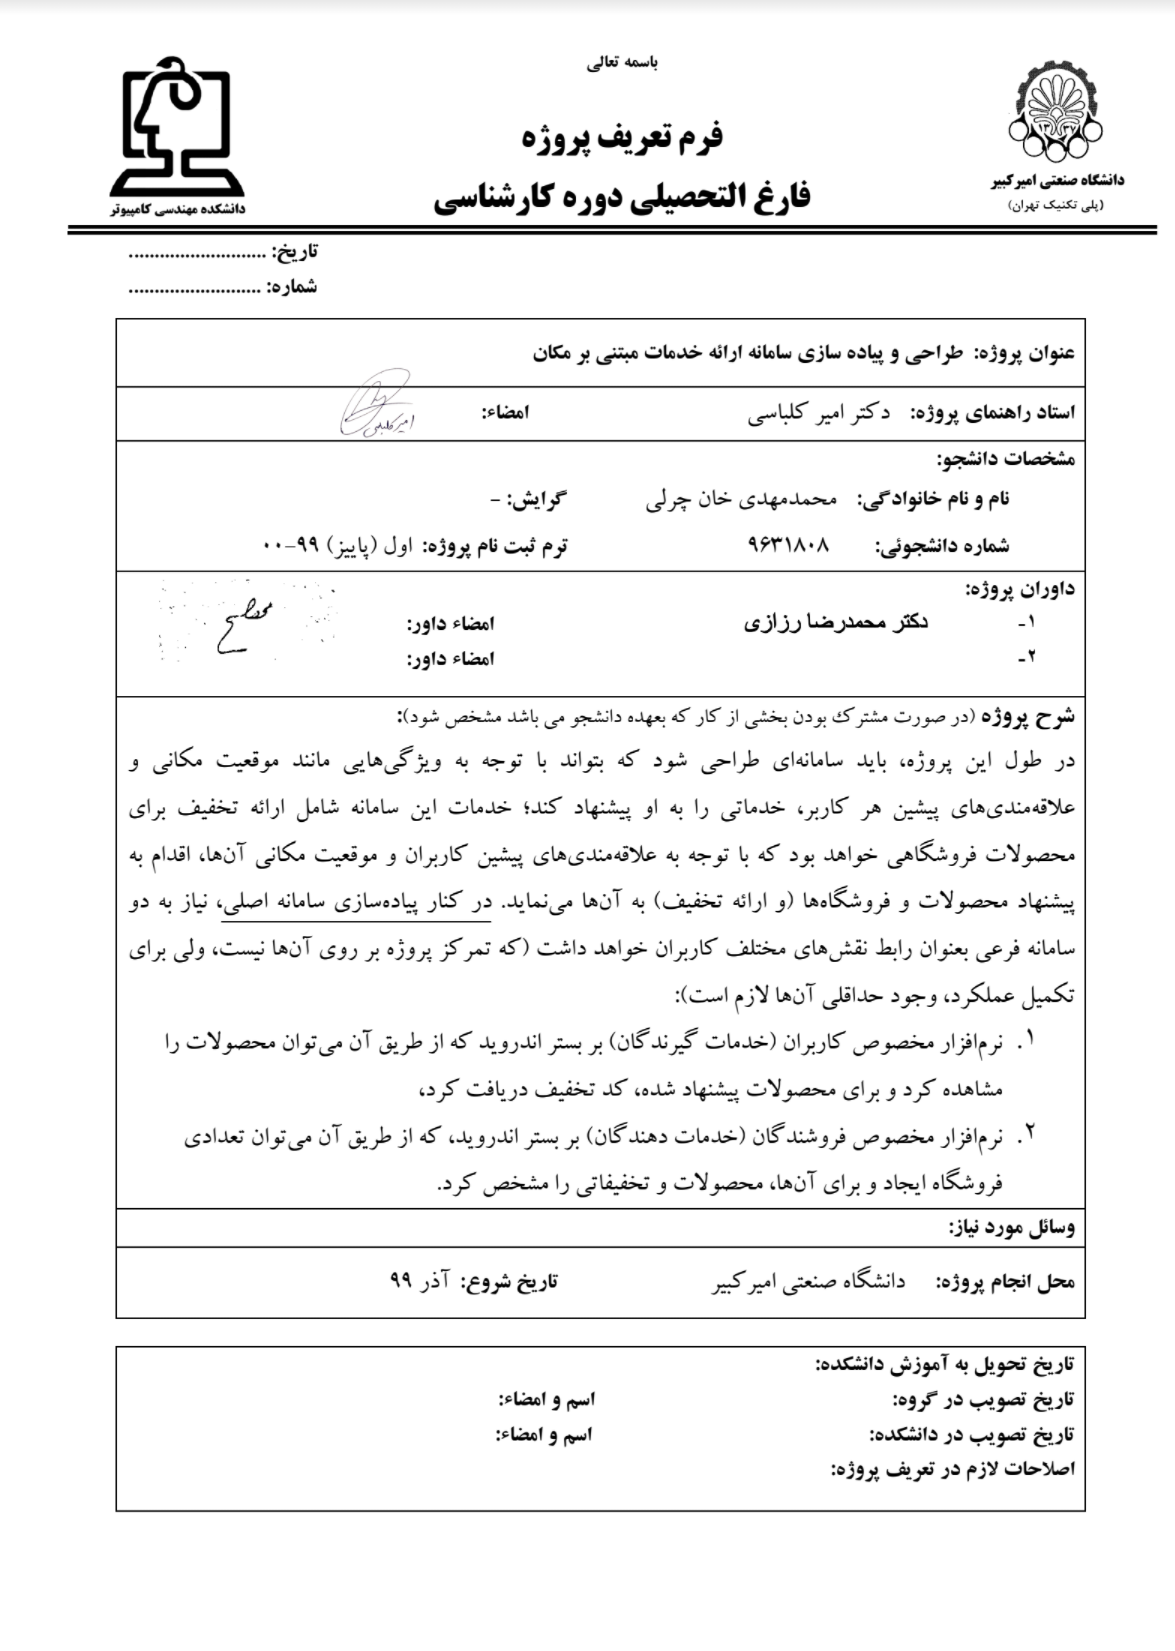
\includegraphics[scale=0.8]{taeid}
% \end{figure}

% \captionsetup[figure]{list=yes}

%%%%%%%%%%%%%%%%%%%%%%%%%%%%%%%%%%%%%%%%%%%%%%%%%%%%%%%%%%%%%%%%%%%%%%%%%%%%%%%%%%%%%%%%%%%%%%%%%%
%%%%%%%%%%%%%%%%%%%%%%%%%%%%%%%%%%%%%%%%%%%%%%%%%%%%%%%%%%%%%%%%%%%%%%%%%%%%%%%%%%%%%%%%%%%%%%%%%%
\newpage
\thispagestyle{empty}
\begin{picture}(50,50)
  \put(17,0){
\includegraphics[scale=1.1]{fa-logo}}
  \put(4.5,-13){\footnotesize{دانشگاه صنعتی امیرکبیر}}
  \put(10.5,-27){\footnotesize{(پلی‌تکنیک تهران)}}
  \put(170,30){\bf{به نام خدا}}
  \put(140,-5){\Large\bf{تعهدنامه اصالت اثر}}
  \put(310,0){تاریخ: \datethesis}
\end{picture}

\vspace*{2.5cm}

اينجانب {\bf{\fname\lname}} متعهد می‌شوم که مطالب مندرج در این پایان‌نامه حاصل کار پژوهشی اینجانب تحت نظارت و راهنمایی اساتید دانشگاه صنعتی امیرکبیر بوده و به دستاوردهای دیگران که در این پژوهش از آنها استفاده شده است مطابق مقررات و روال متعارف ارجاع و در فهرست منابع و مآخذ ذکر گردیده است. این پایان‌نامه قبلاً برای احراز هیچ مدرک هم‌سطح یا بالاتر ارائه نگردیده است.

در صورت اثبات تخلف در هر زمان، مدرک تحصیلی صادر شده توسط دانشگاه از درجه اعتبار ساقط بوده و دانشگاه حق پیگیری قانونی خواهد داشت.


کلیه نتایج و حقوق حاصل از این پایان‌نامه متعلق به دانشگاه صنعتی امیرکبیر می‌باشد. هرگونه استفاده از نتایج علمی و عملی، واگذاری اطلاعات به دیگران یا چاپ و تکثیر، نسخه‌برداری، ترجمه و اقتباس از این پایان نامه بدون موافقت کتبی دانشگاه صنعتی امیرکبیر ممنوع است. 
نقل مطالب با ذکر مآخذ بلامانع است.\\
\vspace{2.5cm}


{\centerline {\bf{\fname\lname}}}
\vspace*{.2cm}
{\centerline{امضا}}
%%%%%%%%%%%%%%%%%%%%%%%%%%%%%%%%%
% چنانچه مایل به چاپ صفحات «تقدیم»، «نیایش» و «سپاس‌گزاری» در خروجی نیستید، خط‌های زیر را با گذاشتن ٪  در ابتدای آنها غیرفعال کنید.
% پایان‌نامه خود را تقدیم کنید
% نیایش خود را در فایل زیر بنویسید.
%%\begin{acknowledgementpage}

\vspace{1.5cm}

{\nastaliq
{
 نويسنده پايان‌نامه، درصورت تمايل ميتواند برای سپاسگزاری پايان‌نامه خود را به شخص يا اشخاص و يا ارگان خاصی تقدیم نماید.
}}\end{acknowledgementpage}
\newpage
% سپاسگزاری را در فایل زیر بنویسید.
%%%%%%%%%%%%%%%%%%%%%%%%%%%%%%%%%%%%
\newpage\thispagestyle{empty}
% سپاس‌گزاری
{\nastaliq
سپاس‌گزاری
}
\\[2cm]

 بر خود لازم می‌دانم که از زحمات جناب آقای دکتر محمداعظم خسروی که در مراحل انجام این پروژه به عنوان استاد راهنما و استاد مشاور در کنار بنده بودند و حمایت همه جانبه از من داشتند، تقدیر و تشکر به عمل آورم. امید است که توانسته باشم اندکی از الطافشان را جبران کنم.
 \\
 
از پدر و مادر عزیزم، که بیان تشکر از ایشان، از دامنه‌ی لغات فراگرفته در زندگی‌ام خارج است، کمال تشکر را دارم و امیدوارم ذره‌ای از زحمات بی‌منتشان را جبران کرده باشم.
 \\
 
در پایان از جناب آقای دکتر فرید کاویانی، دکتر امیرحسن آشنایی و مهندسی سعید دیاری بابت راهنمایی‌های بی‌چشم‌داشت و دلسوزانه‌شان، تقدیر و تشکر می‌نمایم.
 














% با استفاده از دستور زیر، امضای شما، به طور خودکار، درج می‌شود.
\signature








%%%%%%%%%%%%%%%%%%%%%%%%%%%%%%%%%%%%%%%%%
%%%%%%%%%%%%%%%%%%%%%%%%%%%%%%%%%کدهای زیر را تغییر ندهید.
\newpage\clearpage

\pagestyle{style2}

\vspace*{-1cm}
\section*{\centering چکیده}
%\addcontentsline{toc}{chapter}{چکیده}
\vspace*{.5cm}
\ffa-abstract
\vspace*{2cm}


{\noindent\large\textbf{واژه‌های کلیدی:}}\par
\vspace*{.5cm}
\fkeywords
% دستور زیر برای شماره گذاری صفحات قبل از فصل اول با حروف ابجد است.
\pagenumbering{alph}
%-----------------------------------------------------------------------------
% فایل زیر دستورات مربوط به نمایش صفحات فهرست مطالب- فهرست اشکال و جداول است.
%{\pagestyle{style2}
%\tableofcontents}\newpage
%
%\listoffigures
\cleardoublepage
%\addtocontents{toc}{\tocheading}
\pagestyle{style6}
\tableofcontents
\pagestyle{style6}
\cleardoublepage
%اگر لیست تصاویر و لیست جداول ندارید ، کدهای زیر را با گذاشتن % در ابتدای آنها، غیرفعال کنید.
\BeginNoToc
%============
\addtocontents{lof}{\lofheading}% add heading to the first page in LoF
\pagestyle{style5}
\listoffigures
\thispagestyle{style5}
%\clearpage
%============
%\addtocontents{lot}{\lotheading}% add heading to the first page in LoT
%\thispagestyle{style4}
%\listoftables
%\thispagestyle{style4}
%============
%\cleardoublepage
%
%\cleardoublepage
%\setcounter{savepage}{\arabic{page}}
%\mainmatter
%\addtocontents{toc}{\tocheading}% add heading to the first page in ToC, after frontmatter entries
\EndNoToc
% در صورت تمایل می‌توانید با فعال کردن دستور بالا، لیست تصاویر را به  پایان‌نامه خود اضافه کنید.
%-------------------------------------------------------------------------symbols(فهرست نمادها)
% وجود لیست نمادها الزامیست.(لطفاً نمادهای خود را جایگذین نمادهای پیش‌فرض کنید.)
%%%%%%%%%%%%%%

{\centering\LARGE\textbf{فهرست نمادها}\par}%

\pagenumbering{alph}
\setcounter{page}{\thesavepage}
%\setcounter{page}{6}
\vspace*{1cm}

\pagestyle{style3}
%\thispagestyle{empty}
%\addcontentsline{toc}{chapter}{فهرست نمادها}
\symb{\text{ نماد}}{مفهوم}
\\
%مقادیر بالا را تغییر ندهید
%%%%%%%%%%%%%%%%%%%%%%%%%%%%%%%%%%%%%%%%%%%%%%%%%%%%%%%%%
\symb{\mathbb{R}^n}{
فضای اقلیدسی با بعد $n$
}
\symb{\mathbb{S}^n}{
کره یکه $n$ بعدی
}
\symb{M^m}{
خمینه $m$-بعدی $M$
}
\symb{\mathfrak{X}(M)}{
جبر میدان‌های  برداری هموار روی $M$
}
\symb{\mathfrak{X}^1(M)}{
مجموعه میدان‌های برداری هموار یکه روی $(M,g)$ 
}
\symb{\Omega^p(M)}{
مجموعه $p$-فرمی‌های روی خمینه $M$
}
\symb{Q}{
اپراتور ریچی
}
\symb{\mathcal{R}}{
تانسور انحنای ریمان
}
\symb{ric}{
تانسور ریچی
}
\symb{L}{
مشتق لی
}
\symb{\Phi}{
2-فرم اساسی خمینه تماسی
}
\symb{\nabla}{
التصاق لوی-چویتای
}
\symb{\Delta}{
لاپلاسین ناهموار
}
\symb{\nabla^*}{
عملگر خودالحاق صوری القا شده از التصاق لوی-چویتای
}
\symb{g_s}{
متر ساساکی
}
\symb{\nabla}{
التصاق لوی-چویتای وابسته به متر ساساکی
}
\symb{\Delta}{
عملگر لاپلاس-بلترامی روی $p$-فرم‌ها
}

%%%%%%%%%%%%%%%%%%%%%%%%%%%%%%%%%%%%%%%

\thispagestyle{style3}
\newpage
%\pagestyle{style1}
%%%%%%%%%%%%%%%%%%%%%%%%%%%%%%%%%%%%


\pagenumbering{arabic}
\pagestyle{style1}
%--------------------------------------------------------------------------chapters(فصل ها)
%
\chapter{مقدمه}

\section{زیربخش مقدمه}

دنتردتشی برتنش ر قرنس رند ردن رتنقدبقدتدلتمشنقلد
\chapter{سخت‌افزار و الکترونیک}

همانطور که گفته شد، این پروژه شامل سه قسمت اصلی سخت‌افزار، مکانیک و نرم‌افزار است. در این فصل، به تشریح سخت‌افزار می‌پردازیم.

\section{فیبر مدارچاپی}
	فیبر مدار چاپی یا \pcb\footnote{\lr{Printed Circiut Board}} صفحه‌ای است معمولا از جنس فیبر \lr{FR-4} که با دو لایه‌ی نازک مس (معمولا به ضخامت 35 میکرون) در طرفین پوشیده است. طرحی که طراح به کارخانه‌ی چاپ \pcbf ارسال می‌کند روی این ورقه‌ها پیاده می‌شود. سپس لایه‌ی محافظ معمولا سبز رنگ به نام \lr{Solder mask} روی آن اضافه می‌شود که برای زیبایی بخشی به کار و محافظت از مس در مقابل خوردگی و اکسایش است.
	
	در این پروژه از یک \pcbf چهارلایه استفاده شده است. به دلیل فشردگی بالای طرح و قطعات، همچنین برای بهبود کیفیت سیگنال‌ها و کاهش اثر نویز، دو صفحه‌ی زمین در لایه‌های 2 و 3 تعبیه شده است. این صفحه‌ها با کوتاه کردن مسیر جریان برگشتی باعث بهبود کیفیت سیگنال و کاهش اثر نویز می‌شوند. همچنین تأثیر چشم‌گیری در سهولت مسیرکشی \pcbf دارند.

 \pcbf 
 های این پروژه -به رایگان- توسط شرکت \lr{PCBWay}\cite{PCBWay} چاپ شده است که از بزرگترین و مجهزترین کارخانه‌های چاپ \pcbf در کشور چین است.
 
 شکل \ref{fig:pcb_design}  تصویر \pcbf طراحی شده در نرم‌افزار \lr{Altium Designer} را نشان می‌دهد. تصاویر مربوط به \pcbf در شکل \ref{fig:pcb-images} قابل مشاهده است.
 
 \begin{figure}[h]
 	\centering
 	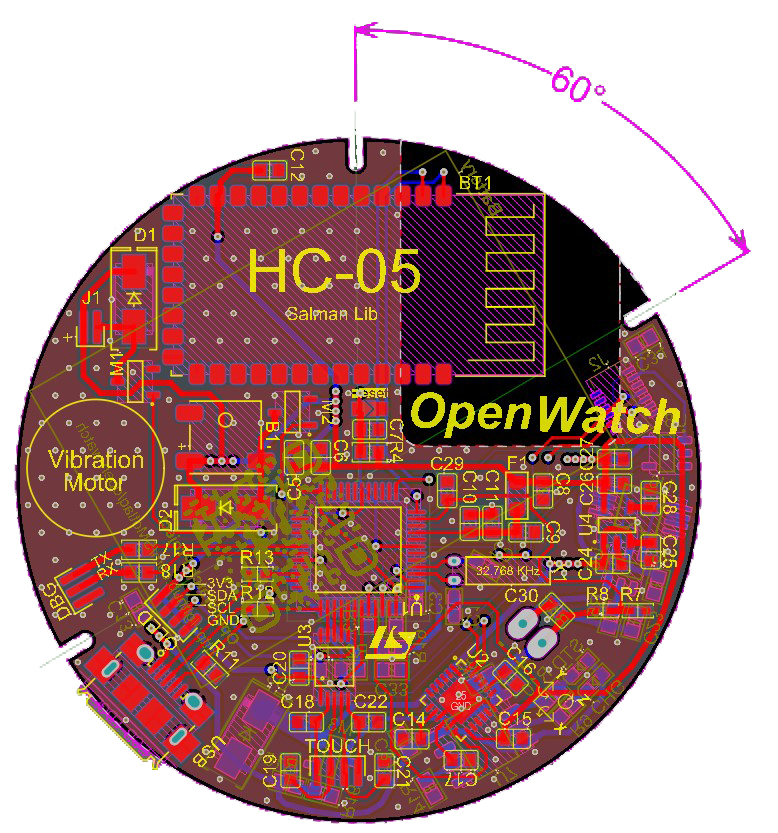
\includegraphics[width=0.5\textwidth]{pcb_main}
 	\caption{\pcbf طراحی شده در نرم‌افزار \lr{Altium Designer}}
 	\label{fig:pcb_design}
 \end{figure}
 
 \begin{figure}[h]
 	\centering
 	\begin{subfigure}{0.45\textwidth}
 		\centering
 		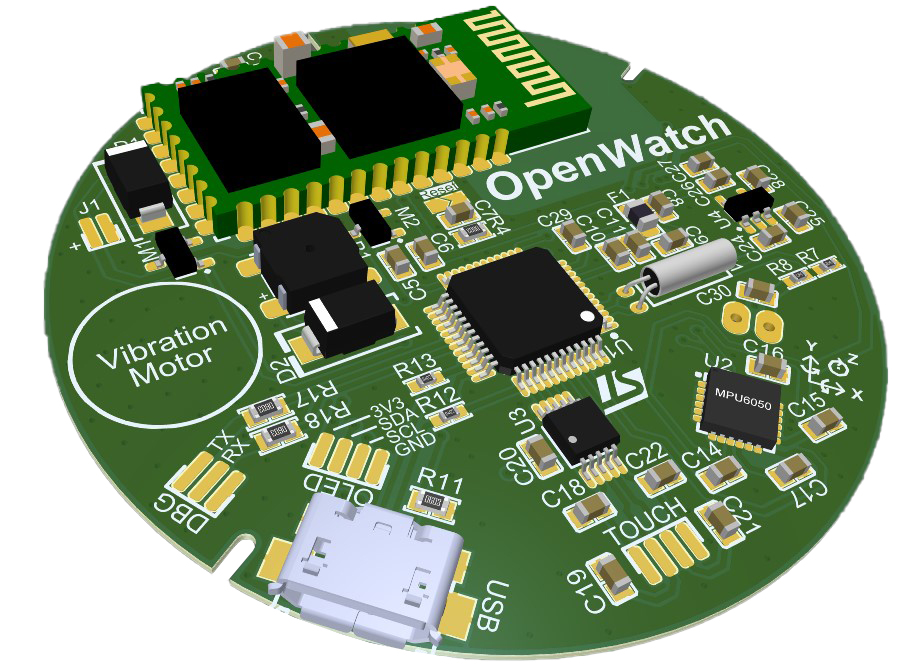
\includegraphics[width=0.9\linewidth]{pcb_main_3d}
 		\caption{نمای سه بعدی طرح - رو}
 		%\label{fig:stm32_image}
 	\end{subfigure}
 	\begin{subfigure}{0.45\textwidth}
 		\centering
 		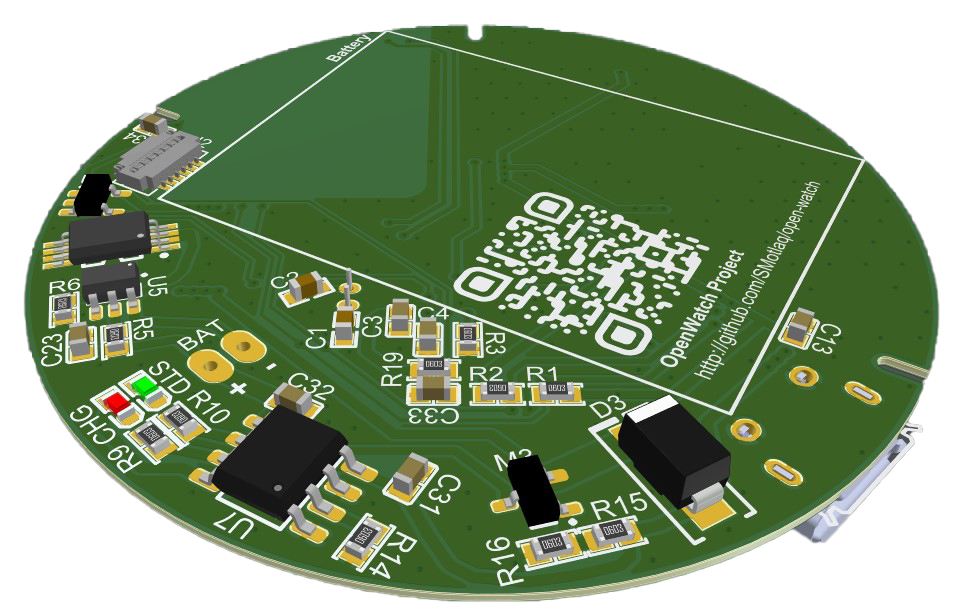
\includegraphics[width=\linewidth]{pcb_main_3d_back}
 		\caption{نمای سه بعدی طرح - پشت}
 		%\label{fig:stm32_real}
 	\end{subfigure}\\
	\begin{subfigure}{0.45\textwidth}
		\centering
		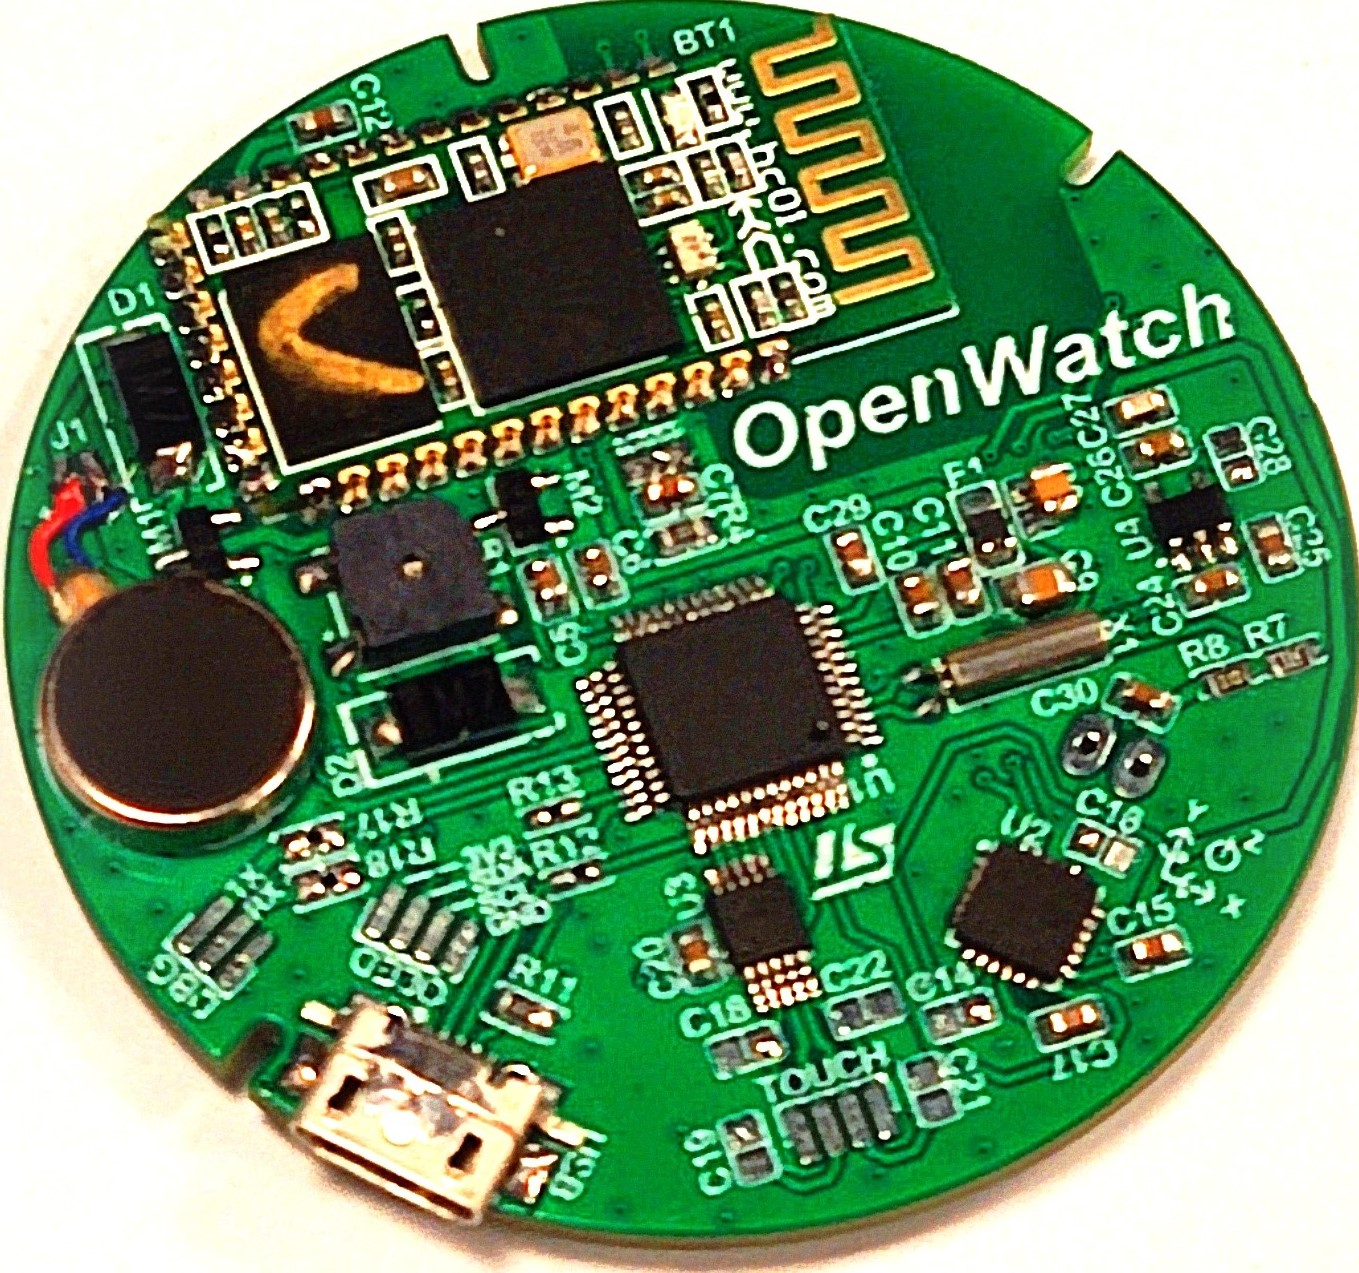
\includegraphics[width=0.9\linewidth]{pcb_real_mounted}
		\caption{\pcbf مونتاژ شده}
		%\label{fig:stm32_image}
	\end{subfigure}
	\begin{subfigure}{0.45\textwidth}
		\centering
		\includegraphics[width=0.9\linewidth]{pcb_real_raw}
		\caption{\pcbf خام}
		%\label{fig:stm32_image}
	\end{subfigure}
 	\caption{تصاویری از \pcbf پروژه}
 	\label{fig:pcb-images}
 \end{figure}
 
\section{هسته‌ی پردازشی} \label{sec:mcu}
برای انتخاب پردازنده‌ی مناسب باید موارد ذیل را مدنظر داشت:
\begin{enumerate}
	\item مقدار حافظه‌ی فلش\footnote{\lr{Flash}}:\\
	برنامه‌ای که برای پردازنده نوشته می‌شود در حافظه‌ی فلش ذخیره می‌شود. پس این حافظه مشخص می‌کند چه حجمی از برنامه در این پردازنده جا می‌شود.
	\item مقدار حافظه‌ی رم\footnote{\lr{RAM}}:\\
	این حافظه، یک حافظه‌ی موقت است که متغیرها، اشاره‌گرها\footnote{\lr{Pointers}}، نقطه‌ی بازگشت توابع و مقادیر ثبات‌ها\footnote{\lr{Registers}} به طور موقت در آن نوشته می‌شود. مقدار رم موردنیاز باید با توجه به حجم متغیرها و پیچیدگی عملیاتی و محاسباتی برنامه تعیین شود.
	\item تعداد پایه‌ها و مدارهای واسط\footnote{\lr{Peripherals}}:\\
	پردازنده‌های مختلف تنوع زیادی در نوع و تعداد مدارهای واسط ارائه می‌دهند. با توجه به تعداد سخت‌افزارهای جانبی، باید تعداد پایه و نوع مدارهای واسط موردنیاز تعیین شود.
	\item پکیج\footnote{\lr{Package}}:\\
	پکیج‌های مختلف نمایانگر شکل ظاهری پردازنده است. برخی پکیج‌ها ابعاد بزرگی دارند و برخی دیگر به قدری کوچک هستند که پایه‌های پردازنده در زیر تراشه تعبیه می‌شوند تا فضای کمتری اشغال کند. در انتخاب پکیج باید محدودیت فضای \pcbf را مدنظر قرار داد.
	\item موجودی بازار:\\
	یکی از مهمترین چالش‌های مهندسان الکترونیک در ایران، موجودی بازار است. خیلی از قطعاتی که طراح به آن‌ها نیاز دارد در بازار ایران پیدا نمی‌شود یا قیمت بالایی دارد. یا باید به وارد کردن قطعه و تاخیر چند ماهه تن داد یا باید طرح را عوض کرد تا با قطعات موجود در بازار قابل پیاده‌سازی باشد.
	\item قیمت:\\
	بدیهی است که یکی از قیود طراحی، قیمت تمام شده است. طراح باید در انتخاب پردازنده طوری عمل کند که با کمترین قیمت، بهترین تطابق را با قیود بالا ایجاد کند.
\end{enumerate}

در نهایت با بررسی موارد فوق، پردازنده‌ی انتخاب شده در این پروژه \lr{STM32F030C8} است. این پردازنده محصول شرکت \lr{ST} که هسته‌ی \lr{ARM Cortex-M0} 32 بیتی دارد. شکل \ref{fig:stm32_image} تصویر واقعی این پردازنده و شکل \ref{fig:stm32_real} تصویر آن را بر روی \pcbf ساعت نشان می‌دهد.

\begin{figure}[h]
	\centering
	\begin{subfigure}{0.35\textwidth}
		\centering
		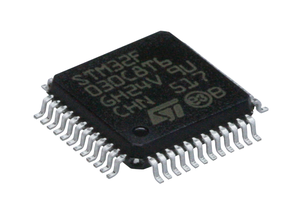
\includegraphics[width=\linewidth]{stm32f030}
		\caption{جداگانه}
		\label{fig:stm32_image}
	\end{subfigure}
	\begin{subfigure}{0.35\textwidth}
		\centering
		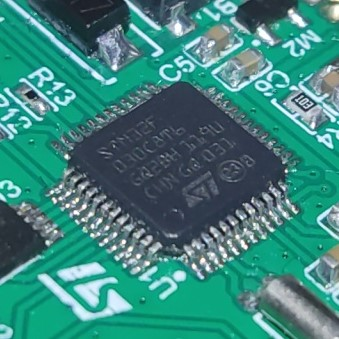
\includegraphics[width=\linewidth]{stm32f030_real}
		\caption{مونتاژ شده روی برد پروژه}
		\label{fig:stm32_real}
	\end{subfigure}
	\caption{تصاویری از پردازنده \lr{STM32F030}}
	\label{fig:stm32}
\end{figure}

شکل \ref{fig:sch-mcu} شماتیک مداری بخش پردازنده را نشان می‌دهد. یک کریستال 32768 هرتزی وظیفه‌ی تنظیم فرکانس بخش
 \lr{RTC}\footnote{\lr{Real Time Clock}}
  را بر عهده دارد. ساعت سیستم توسط این واحد ذخیره و تنظیم می‌شود. تغذیه‌ی بخش 
  \lr{ADC}\footnote{\lr{Analog to Digital Converter}}
  توسط چند خازن و یک فریت‌بید\footnote{\lr{Ferrite Bead}} فیلتر شده است. تغذیه‌ی خود پردازنده نیز توسط 4 خازن (مطابق با دستور کارخانه سازنده) فیلتر شده است.

\begin{figure}
	\centering
	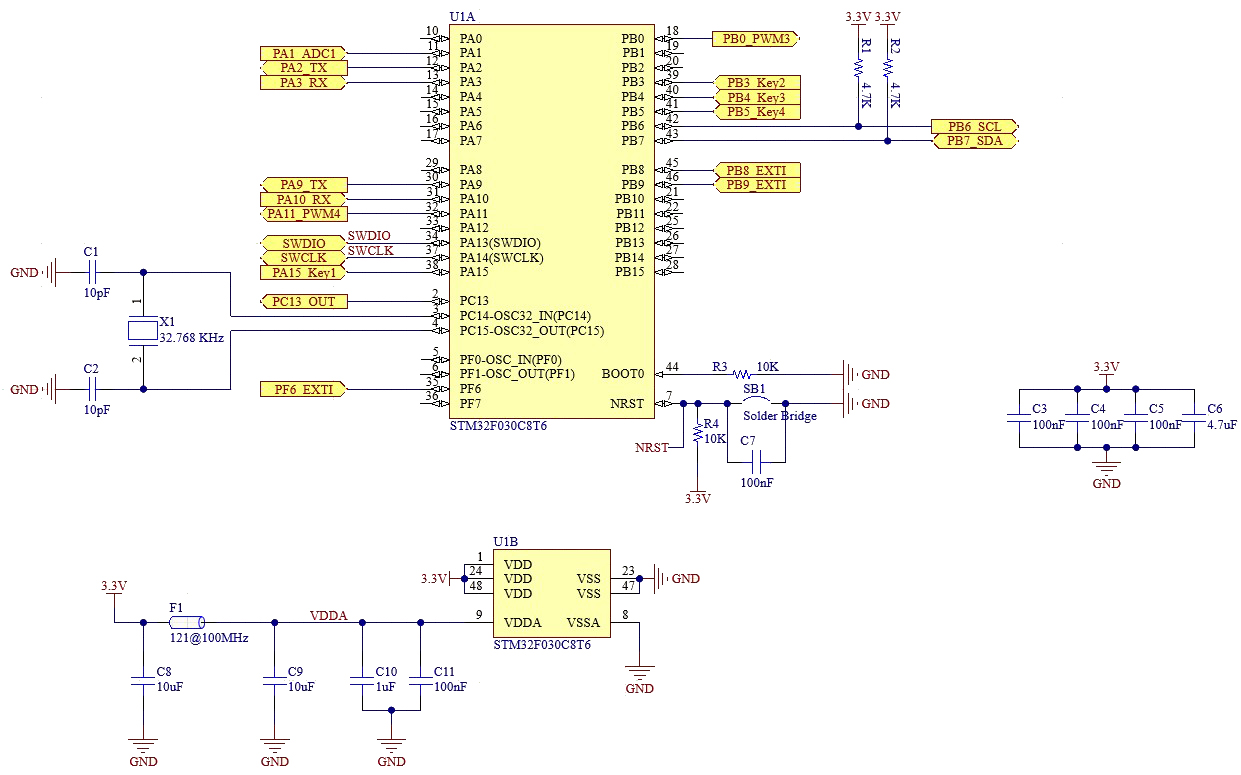
\includegraphics[width=\textwidth]{sch_mcu}
	\caption{شماتیک مربوط به بخش ریزپردازنده}
	\label{fig:sch-mcu}
\end{figure}


\section{درگاه بلوتوث}
ارتباط ساعت با تلفن‌همراه از طریق درگاه بلوتوث\footnote{\lr{Bluetooth}} است. قیود انتخاب بلوتوث هم تا حدی مشابه قیود انتخاب پردازنده (ابتدای بخش \ref{sec:mcu}) است. با در نظر گرفتن شرایط بازار، قیمت و عملکرد ماژول‌های مختلف، نهایتا ماژول \lr{HC-05} برای این پروژه انتخاب شد. شکل \ref{fig:hc05_image} تصویر این ماژول و شکل \ref{fig:hc05_real} تصویر آن را بر روی \pcbf ساعت نشان می‌دهد.

یکی از نکات مهمی که در طراحی \pcbf برای ماژول‌های مخابراتی وجود دارد این است که در نزدیکی آنتن این ماژول‌ها نباید هادی جریان الکتریکی وجود داشته باشد. در غیر این صورت خاصیت خازنی بین آنتن و این هادی باعث تغییر مشخصه‌های آنتن می‌شود و باعث اختلال در عملکرد آنتن می‌گردد. همانطور که در شکل \ref{fig:pcb_design} مشاهده می‌شود، مس‌های اطراف آنتن  حذف شده‌اند تا عملکرد بلوتوث دچار مشکل نشود.

\begin{figure}[h]
	\centering
	\begin{subfigure}{0.45\textwidth}
		\centering
		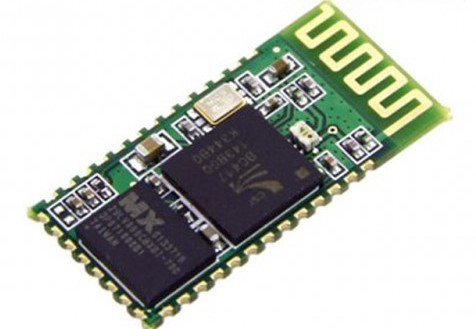
\includegraphics[width=\linewidth]{hc05_real}
		\caption{جداگانه}
		\label{fig:hc05_image}
	\end{subfigure}
	\begin{subfigure}{0.45\textwidth}
		\centering
		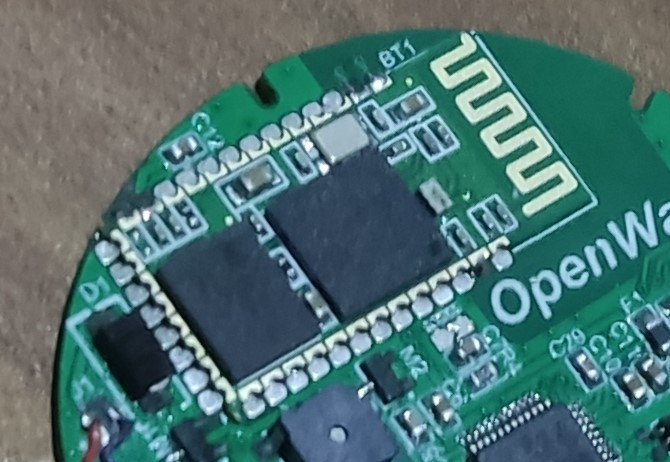
\includegraphics[width=\linewidth]{hc05_mounted}
		\caption{مونتاژ شده روی برد پروژه}
		\label{fig:hc05_real}
	\end{subfigure}
	\caption{تصاویری از ماژول بلوتوث \lr{HC-05}}
	\label{fig:hc05}
\end{figure}

شکل \ref{fig:sch-blue} شماتیک مداری بخش بلوتوث را نشان می‌دهد. پروتکل ارتباطی این ماژول با پردازنده پروتکل
 \lr{UART}\footnote{\lr{Universal Asynchronous Receiver-Transmitter}}
است که با دو پین \lr{RX} و \lr{TX} به پردازنده متصل می‌شود. پریفرال \lr{UART2} در پردازنده به ارتباط با بلوتوث اختصاص دارد. تغذیه‌ی ماژول نیز با یک خازن 100 نانوفارادی فیلتر شده است.

\begin{figure}[h]
	\centering
	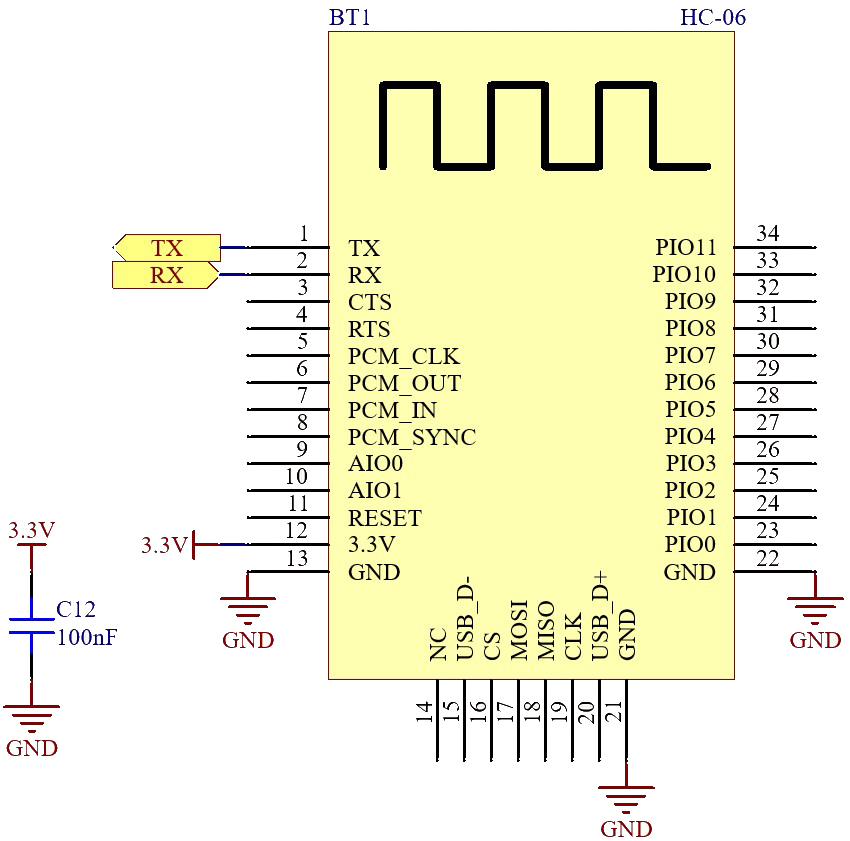
\includegraphics[width=0.6\textwidth]{sch_blue}
	\caption{شماتیک مربوط به بخش بلوتوث}
	\label{fig:sch-blue}
\end{figure}

\section{درگاه ارتباط سریال}
پریفرال \lr{UART1} در پردازنده با دو پین \lr{RX} و \lr{TX} از روی \pcbf خارج شده‌اند. کاربرد این دو پین اشکال‌یابی\footnote{\lr{Debug}} و ارتباط سرعت بالا بین ساعت و رایانه است. این بخش کاربردی در عملکرد کلی ساعت ندارد و صرفا روند توسعه را تسریع می‌کند. شکل \ref{fig:sch_debug} شماتیک مداری و شکل \ref{fig:debug_real} تصویر واقعی این دو پین را نشان می‌دهد.

\begin{figure}[h]
	\centering
	\begin{subfigure}{0.59\textwidth}
		\centering
		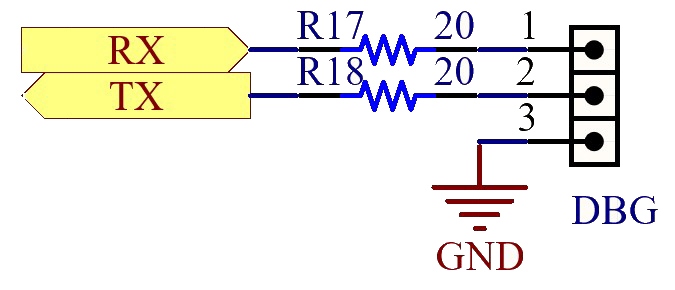
\includegraphics[width=\linewidth]{sch_debug}
		\caption{شماتیک}
		\label{fig:sch_debug}
	\end{subfigure}
	\begin{subfigure}{0.4\textwidth}
		\centering
		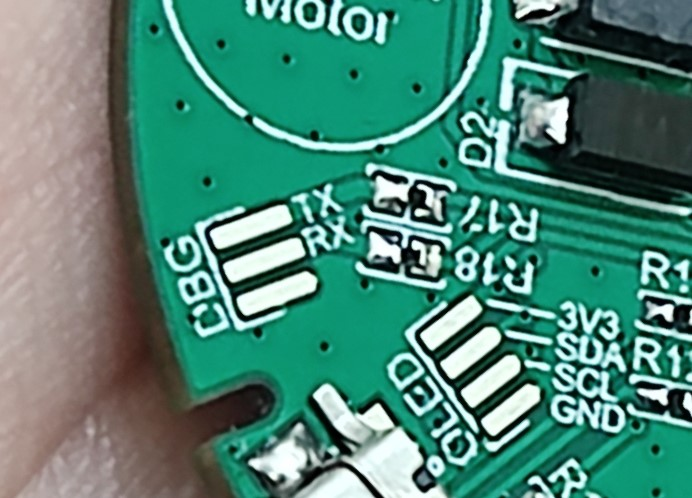
\includegraphics[width=\linewidth]{debug_real}
		\caption{پین‌های مربوطه}
		\label{fig:debug_real}
	\end{subfigure}
	\caption{تصاویر مربوط به درگاه ارتباط سریال}
\end{figure}

\section{حسگر پالس‌اکسی‌متر}
\newpage

\section{حسگر شتاب خطی و سرعت زاویه‌ای}
برای اندازه‌گیری مشخصه‌های حرکتی باید سراغ
\lr{IMU}\footnote{\lr{Inertial Measurement Unit}}ها
رفت. \lr{IMU}ها وسیله‌های الکترونیکی هستند که با استفاده‌ی ترکیبی از شتاب‌سنج‌ها، ژیروسکوپ‌ها و گاهی اوقات مغناطیس‌سنج‌ها، مشخصه‌های حرکتی را اندازه‌گیری و گزارش می‌کنند \cite{IMU}. در این پروژه از حسگر \lr{MPU6050} به این منظور استفاده شده است. این حسگر علی‌رغم قیمت نسبتا پایین، دقت و سرعت مناسبی دارد. مشخصات فنی این حسگر در ضمیمه ؟ موجود است. شکل \ref{fig:gyro_image} تصویر این حسگر و شکل \ref{fig:gyro_real} تصویر آن را بر روی \pcbf ساعت نشان می‌دهد.

\begin{figure}[h]
	\centering
	\begin{subfigure}{0.5\textwidth}
		\centering
		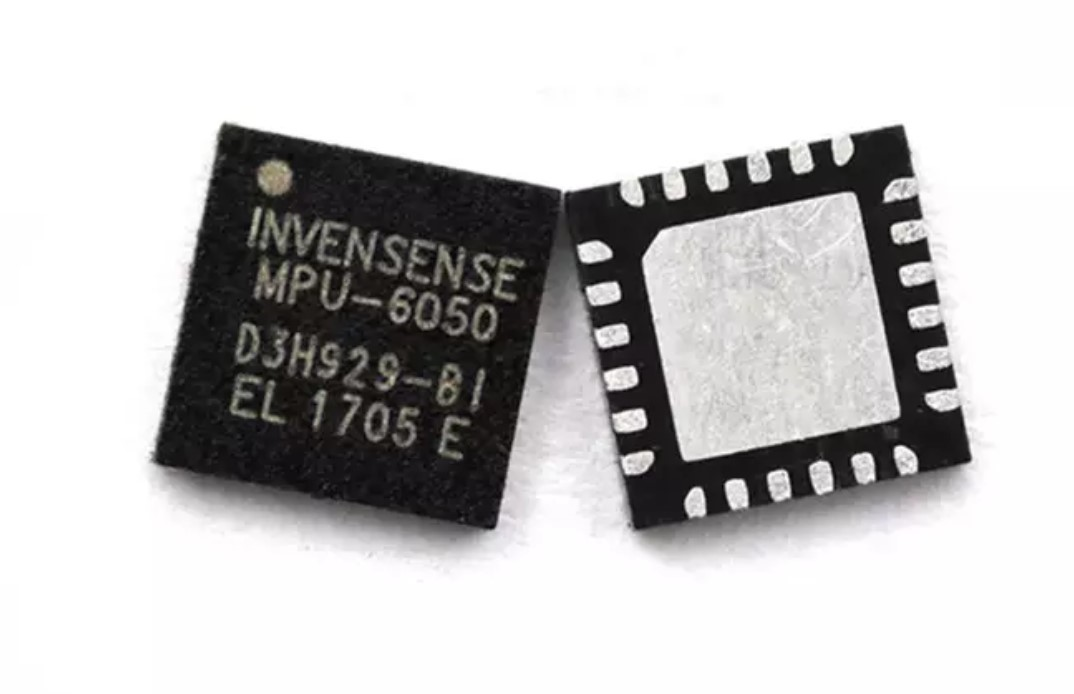
\includegraphics[width=\linewidth]{gyro_image}
		\caption{جداگانه}
		\label{fig:gyro_image}
	\end{subfigure}
	\begin{subfigure}{0.44\textwidth}
		\centering
		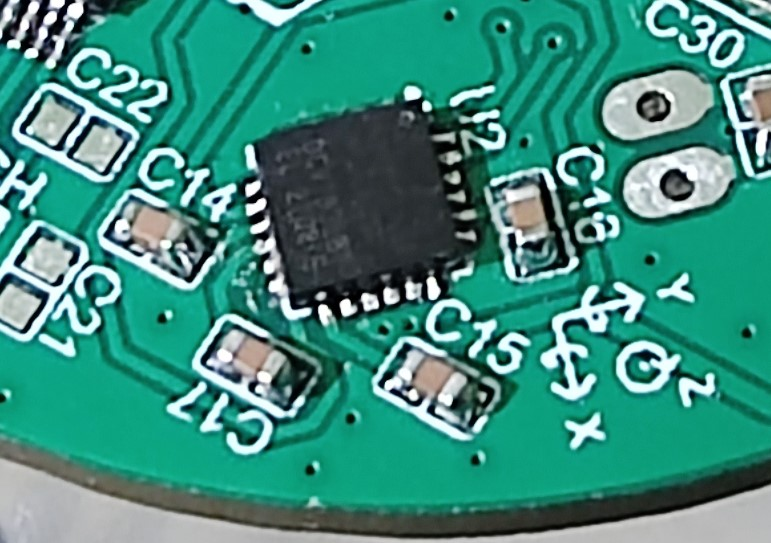
\includegraphics[width=\linewidth]{gyro_real}
		\caption{مونتاژ شده روی برد پروژه}
		\label{fig:gyro_real}
	\end{subfigure}
	\caption{تصاویر حسگر حرکتی}
	%	\label{fig:hc05}
\end{figure}

شکل \ref{fig:sch-gyro} شماتیک مداری حسگر \lr{MPU6050} را نشان می‌دهد. خازن‌ها طبق دستور کارخانه به حسگر متصل شده‌اند. درگاه ارتباطی این حسگر، باس\footnote{\lr{Bus}}
 \lr{I2C}\footnote{\lr{Inter-Integrated Circiut}}
  است. به همین دلیل \lr{I2C1} پردازنده به این حسگر متصل است.

\begin{figure}[h]
	\centering
	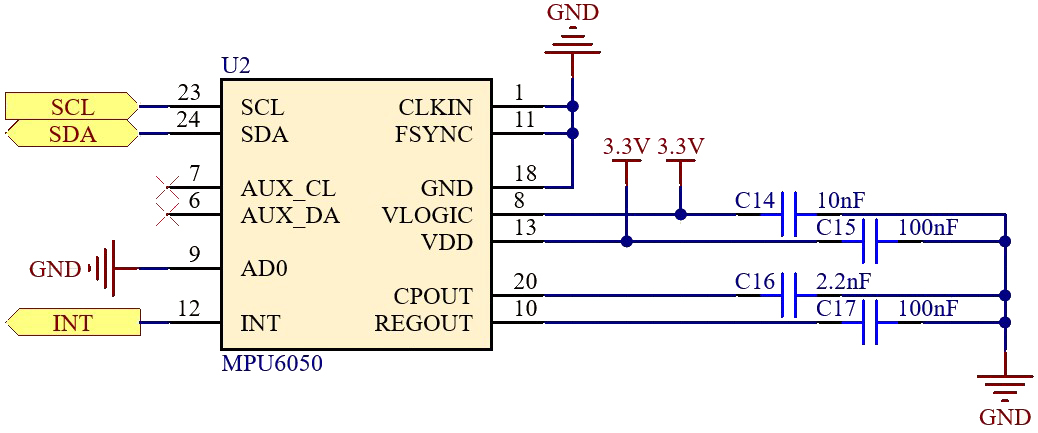
\includegraphics[width=0.8\textwidth]{sch_gyro}
	\caption{شماتیک مربوط به بخش حسگر حرکتی}
	\label{fig:sch-gyro}
\end{figure}

\section{صفحه نمایش}

\section{مدار شارژ و مدیریت توان}

\section{موتور ایجاد لرزش}
برای ایجاد لرزش\footnote{\lr{Vibration}} در ساعت، مشابه تلفن‌های همراه، از یک موتور مخصوص استفاده شده است. موتورهای ایجاد لرزش معمولا یک موتور \lr{DC} ساده هستند که یک بار نامتقارن به آن‌ها متصل است. از آنجا که مرکز جرم این بار خارج از شفت موتور است، چرخش آن باعث ایجاد گشتاوری دوار می‌شود که لرزش را ایجاد می‌کند. شکل \ref{fig:hc05_image} تصویر این موتور و شکل \ref{fig:hc05_real} تصویر آن را بر روی \pcbf ساعت نشان می‌دهد.

\begin{figure}[h]
	\centering
	\begin{subfigure}{0.35\textwidth}
		\centering
		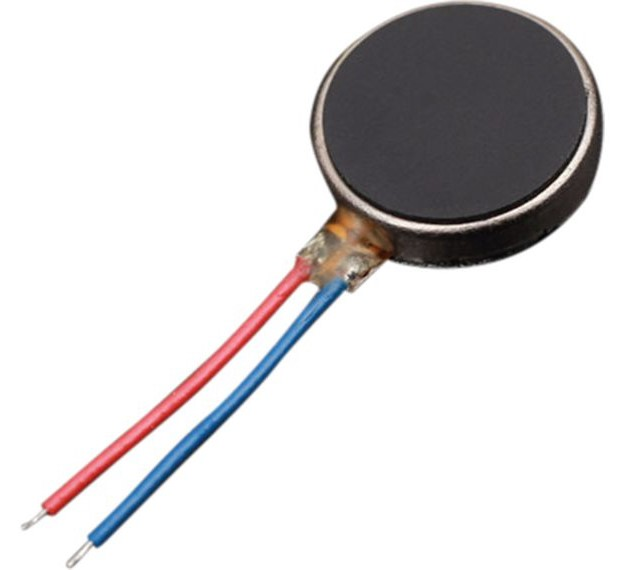
\includegraphics[width=0.75\linewidth]{vib_image}
		\caption{جداگانه}
		\label{fig:vib_image}
	\end{subfigure}
	\begin{subfigure}{0.44\textwidth}
		\centering
		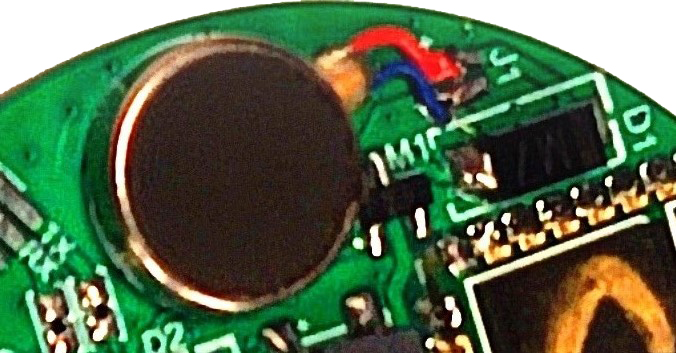
\includegraphics[width=\linewidth]{vib_real}
		\caption{مونتاژ شده روی برد پروژه}
		\label{fig:vib_real}
	\end{subfigure}
	\caption{تصاویر موتور ایجاد لرزش}
%	\label{fig:hc05}
\end{figure}

شکل \ref{fig:sch-vib} شماتیک مداری بخش ایجاد لرزش را نشان می‌دهد. این موتور برای کار به 90 میلی آمپر جریان الکتریکی احتیاج دادر. طبیعتا پردازنده نمی‌تواند این جریان را تأمین کند. لذا از یک سوییچ ماسفت
\footnote{\lr{Metal–Oxide–Semiconductor Field-Effect Transistor}}
 برای قطع و وصل موتور استفاده شده است. دیودی که با موتور موازی شده از ورود جریان برگشتی موتور به ماسفت هنگام خاموش شدن موتور جلوگیری می‌کند. برای کنترل سرعت موتور می‌توان از اعمال موج \lr{PWM}\footnote{\lr{Pulse Width Modulation}} به موتور بهره برد. لذا پایه‌ی فرمان این مدار به خروجی \lr{PWM} تایمر 1 در پردازنده متصل شده است.

\begin{figure}[h]
	\centering
	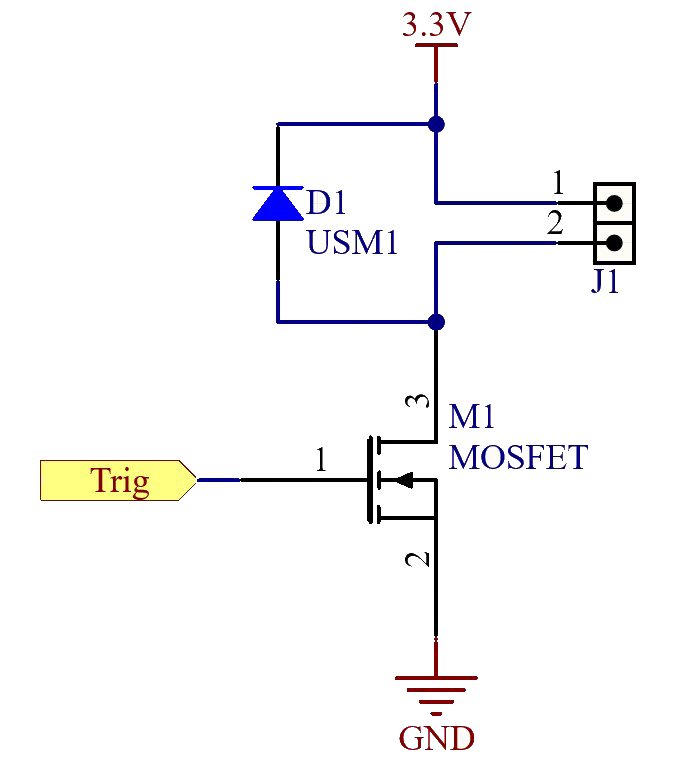
\includegraphics[width=0.52\textwidth]{sch_vib}
	\caption{شماتیک مربوط به بخش ایجاد لرزش}
	\label{fig:sch-vib}
\end{figure}

\section{بازر}

\section{کلیدهای لمسی}
%\chapter{مکانیک و طراحی صنعتی}

این فصل به تشریح بدنه‌ی ساعت و قسمت‌های مکانیکی آن می‌پردازد. قسمت‌های مکانیکی شامل بدنه‌ی اصلی، دریچه‌ی پشتی و نحوه‌ی سرهم شدن قطعات دیگر است.
\section{بدنه‌ی اصلی}
بدنه‌ی اصلی به قسمتی اطلاق می‌شود که از بیرون دیده می‌شود و بزرگترین قطعه است. طراحی این قطعه از صفر در نرم‌افزار \lr{Solid Works} انجام شده است که مطرح‌ترین نرم‌افزار در زمینه‌ی مکانیک و طراحی صنعتی است. برای ساخت بدنه و بخش‌های مکانیکی نیز از فناوری چاپ سه بعدی بهره بردم.

بدنه‌ی اصلی باید:
\begin{multicols}{2}
\begin{enumerate}
	\item محلی برای نصب صفحه نمایش داشته باشد.
	\item  بتواند \pcbf را درون خود جا دهد و مانع چرخش و جابجایی آن شود.
	\item محلی برای اتصال کابل \lr{USB} داشته باشد.
	\item محلی برای جریان هوا داشته باشد. زیرا مدار شارژ باعث افزایش دما می‌شود.
	\item محلی برای اتصال بند داشته باشد.
	\item زیبایی بصری داشته باشد
	\item بیش از حد بزرگ نباشد.
\end{enumerate}
\end{multicols}

برای حصول موارد فوق، چندین نمونه بدنه‌ی مختلف طراحی و چاپ شد تا در هر نسخه، بهبودی نسبت به نسخه‌ی قبلی حاصل شود تا هر چه بهتر شروط فوق ارضا شوند.

\subsection{نسخه‌های اولیه}

در ابتدا یک نمونه‌ی اولیه برای تست کلی بدنه و جانمایی \pcbf و صفحه نمایش طراحی و ساخته شد. تصویر این نمونه‌ی اولیه را می‌توان در شکل ؟ مشاهده کرد.

\begin{figure}[h]
	\centering
	\begin{subfigure}{0.44\textwidth}
		\centering
		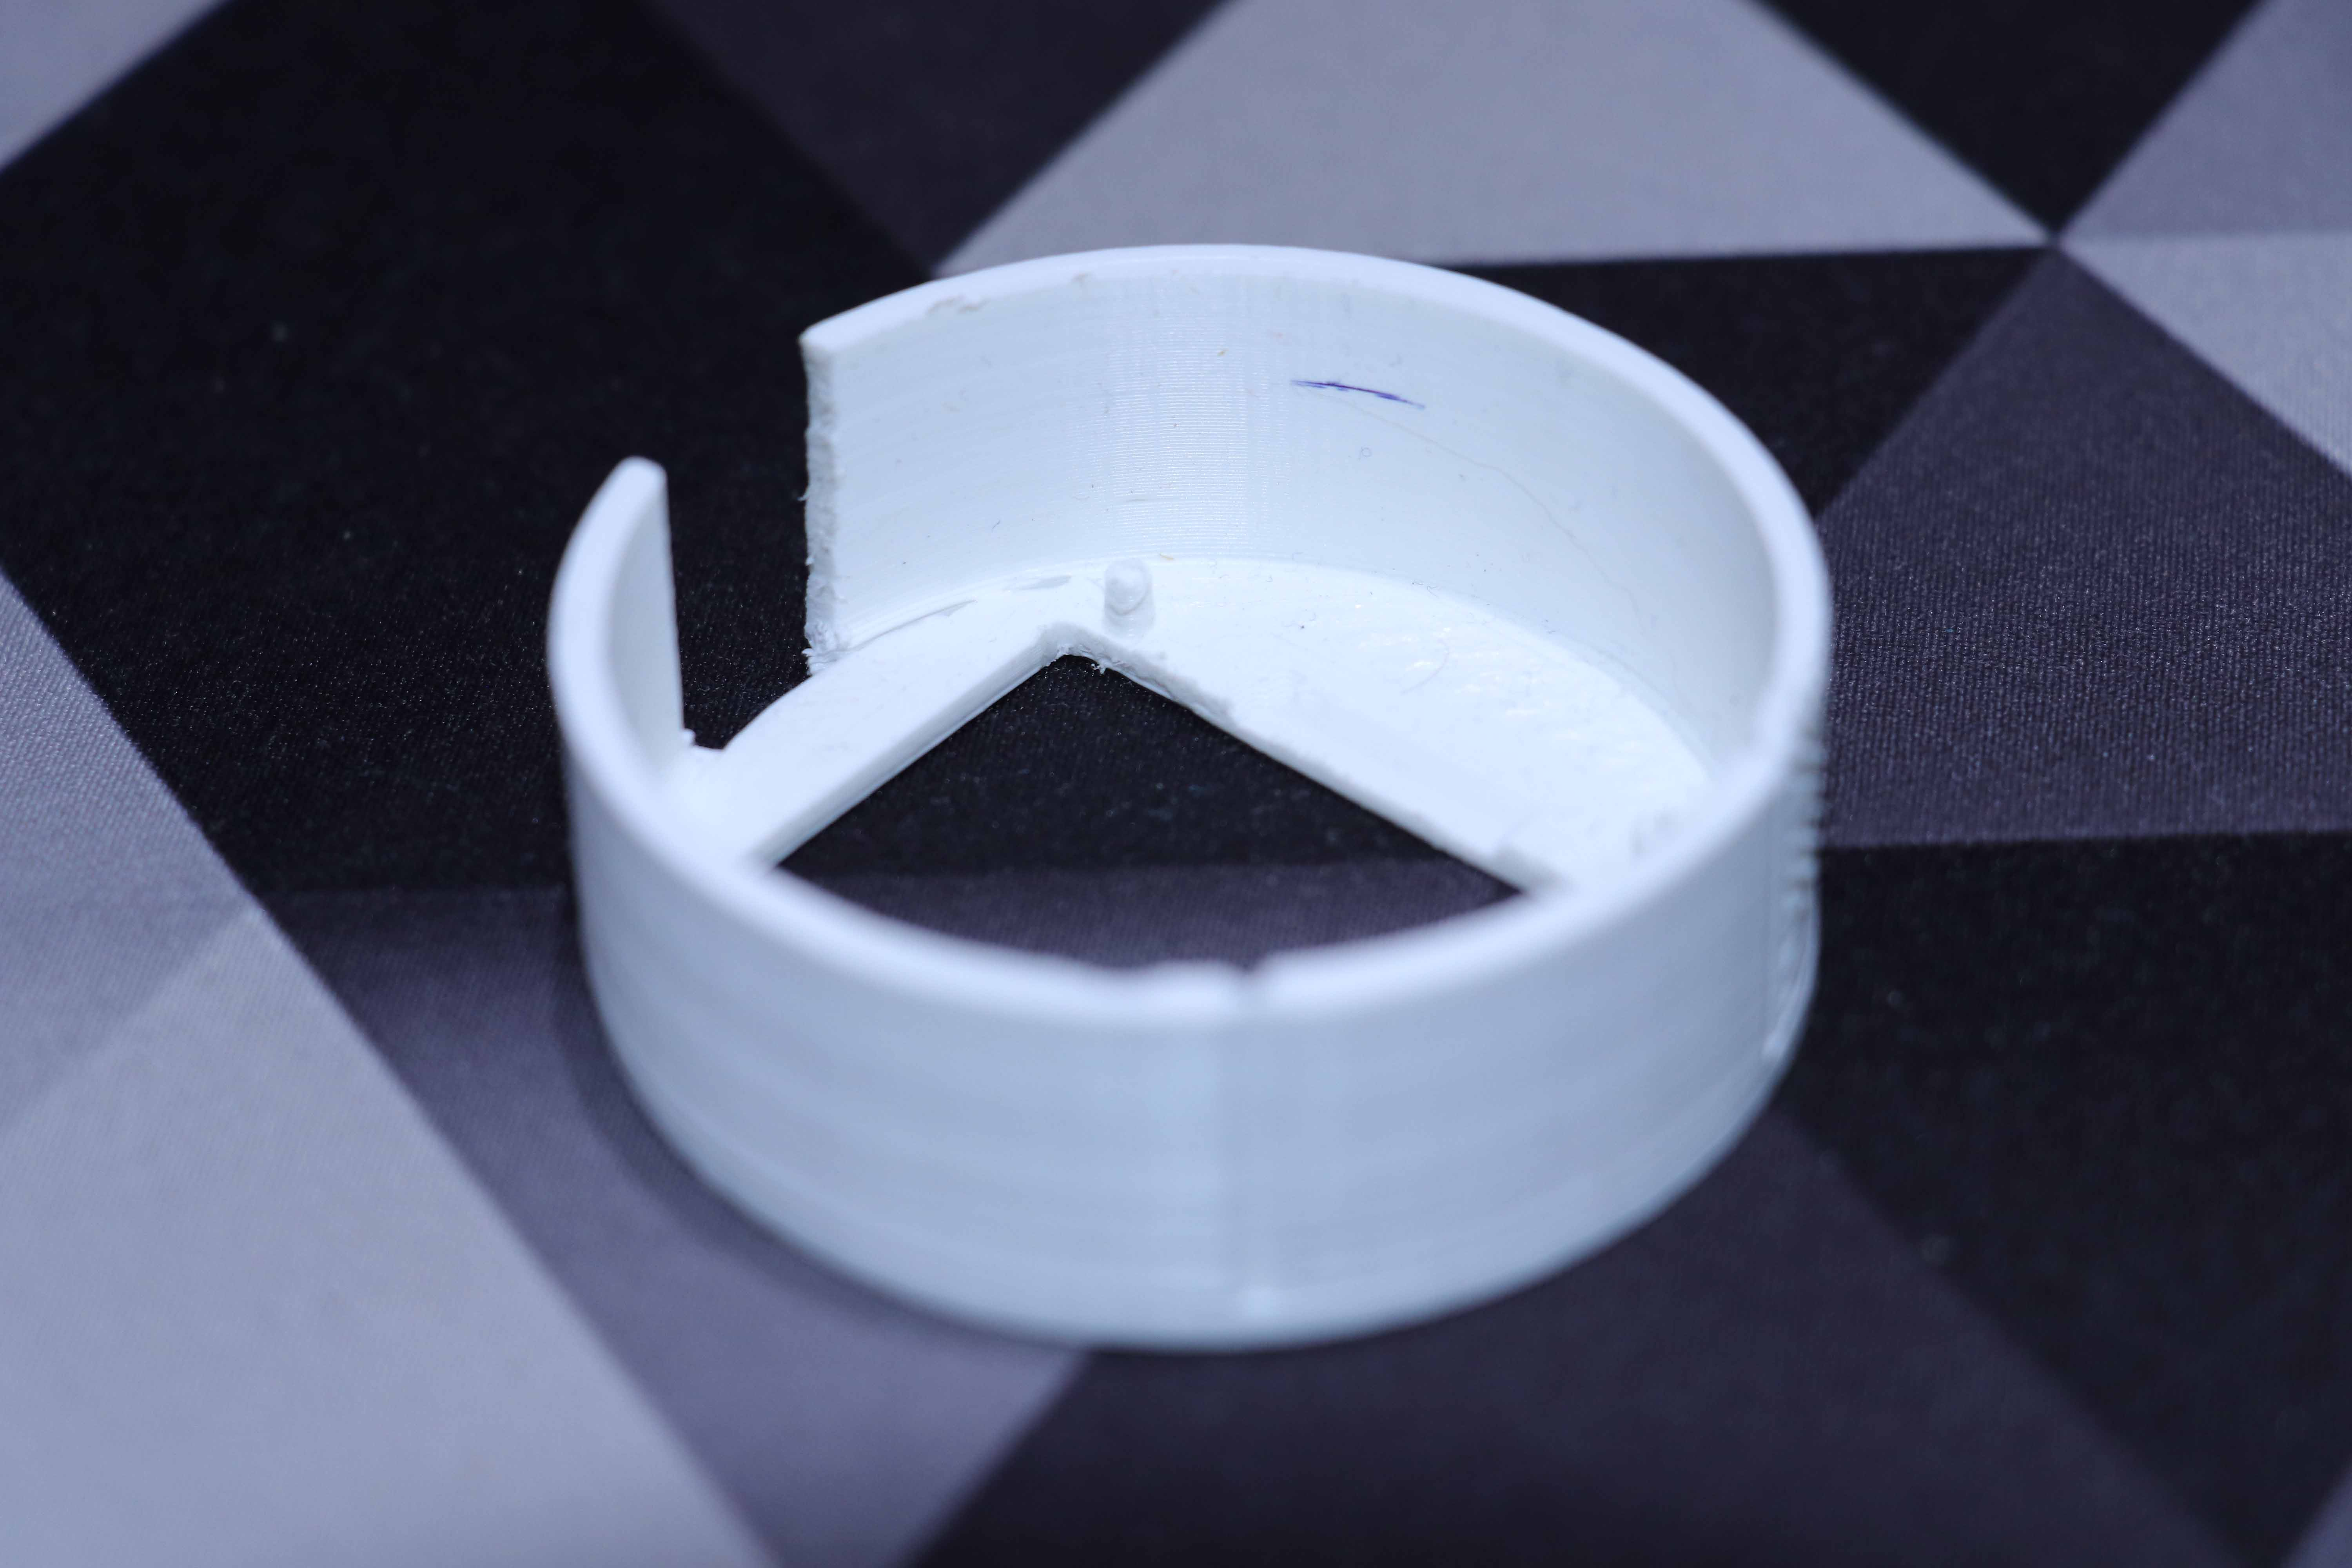
\includegraphics[width=\linewidth]{body_main_v1_back}
		\caption{نمای پشت}
		%\label{fig:oled_image}
	\end{subfigure}
	\begin{subfigure}{0.44\textwidth}
		\centering
		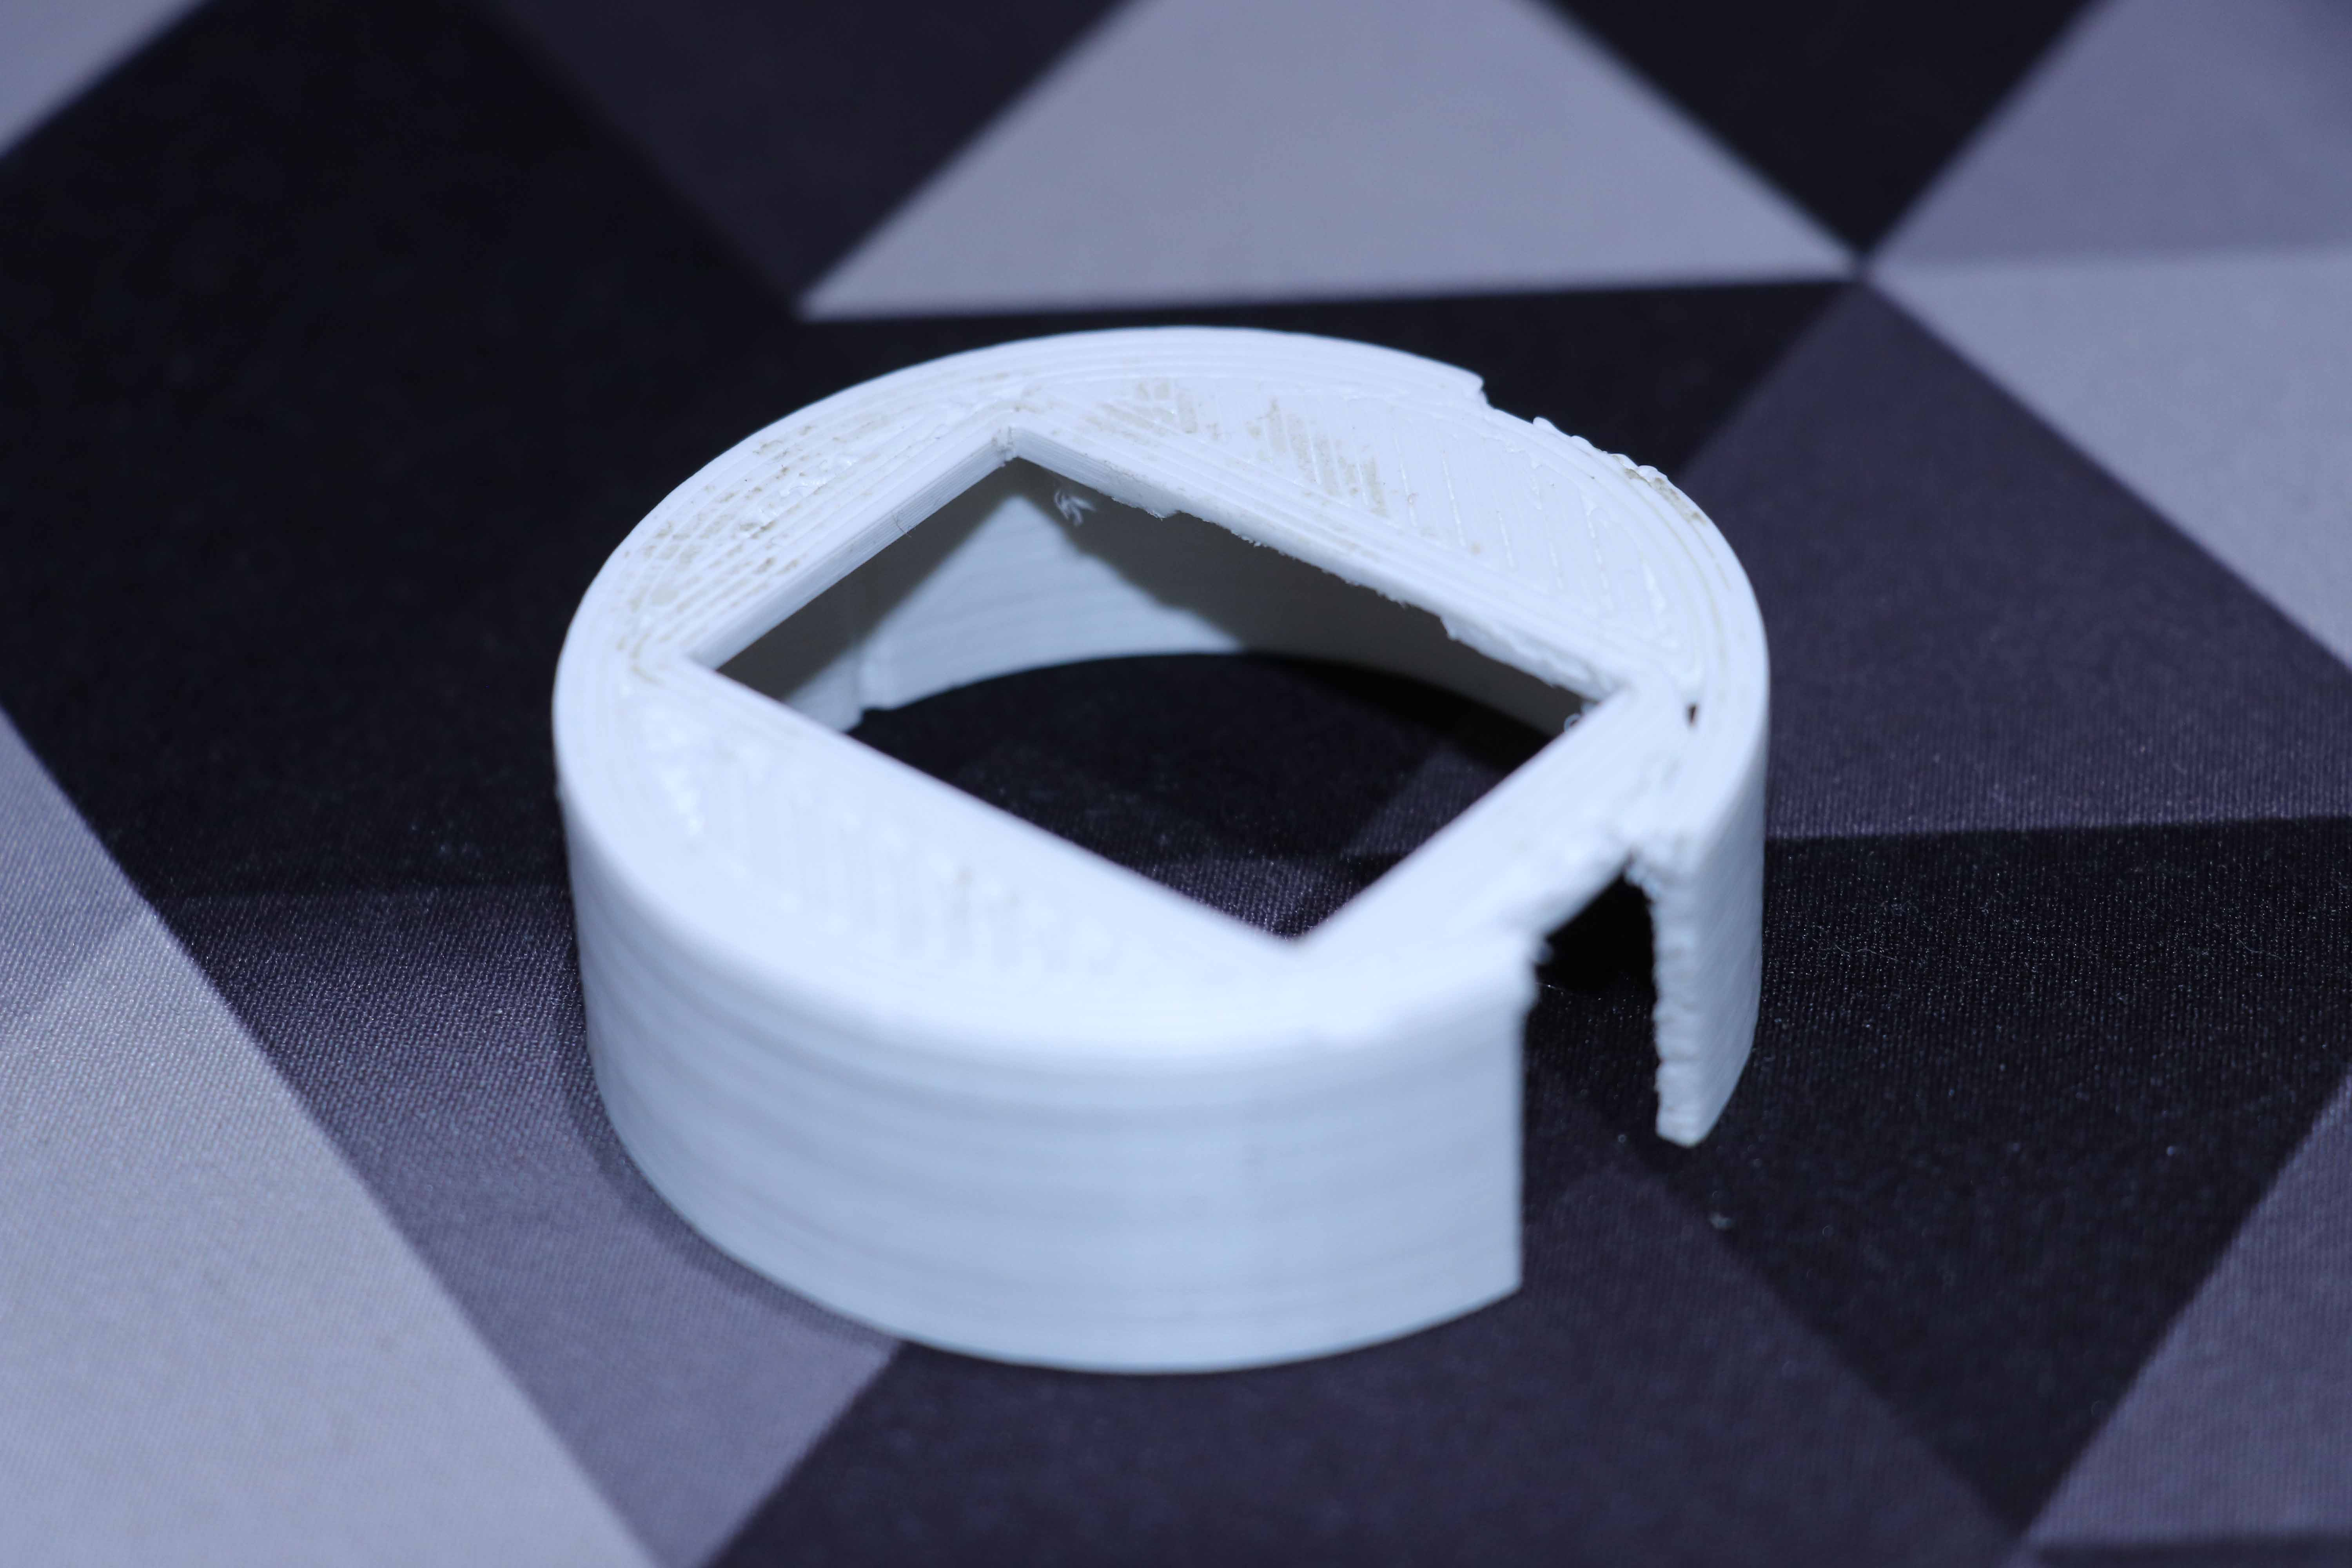
\includegraphics[width=\linewidth]{body_main_v1_front}
		\caption{نمای روبرو}
		%\label{fig:oled_real}
	\end{subfigure}
	\caption{تصاویر بدنه‌ی اصلی نسخه‌ی اول}
	\label{fig:body-v1}
\end{figure}

سپس بعد از نهایی شدن طرح کلی، جزئیات طرح تکمیل شد و نسخه‌ی دوم بدنه به چاپ رسید. تصویر این نسخه در شکل ؟ دیده می‌شود.

\begin{figure}[h]
	\centering
	\begin{subfigure}{0.44\textwidth}
		\centering
		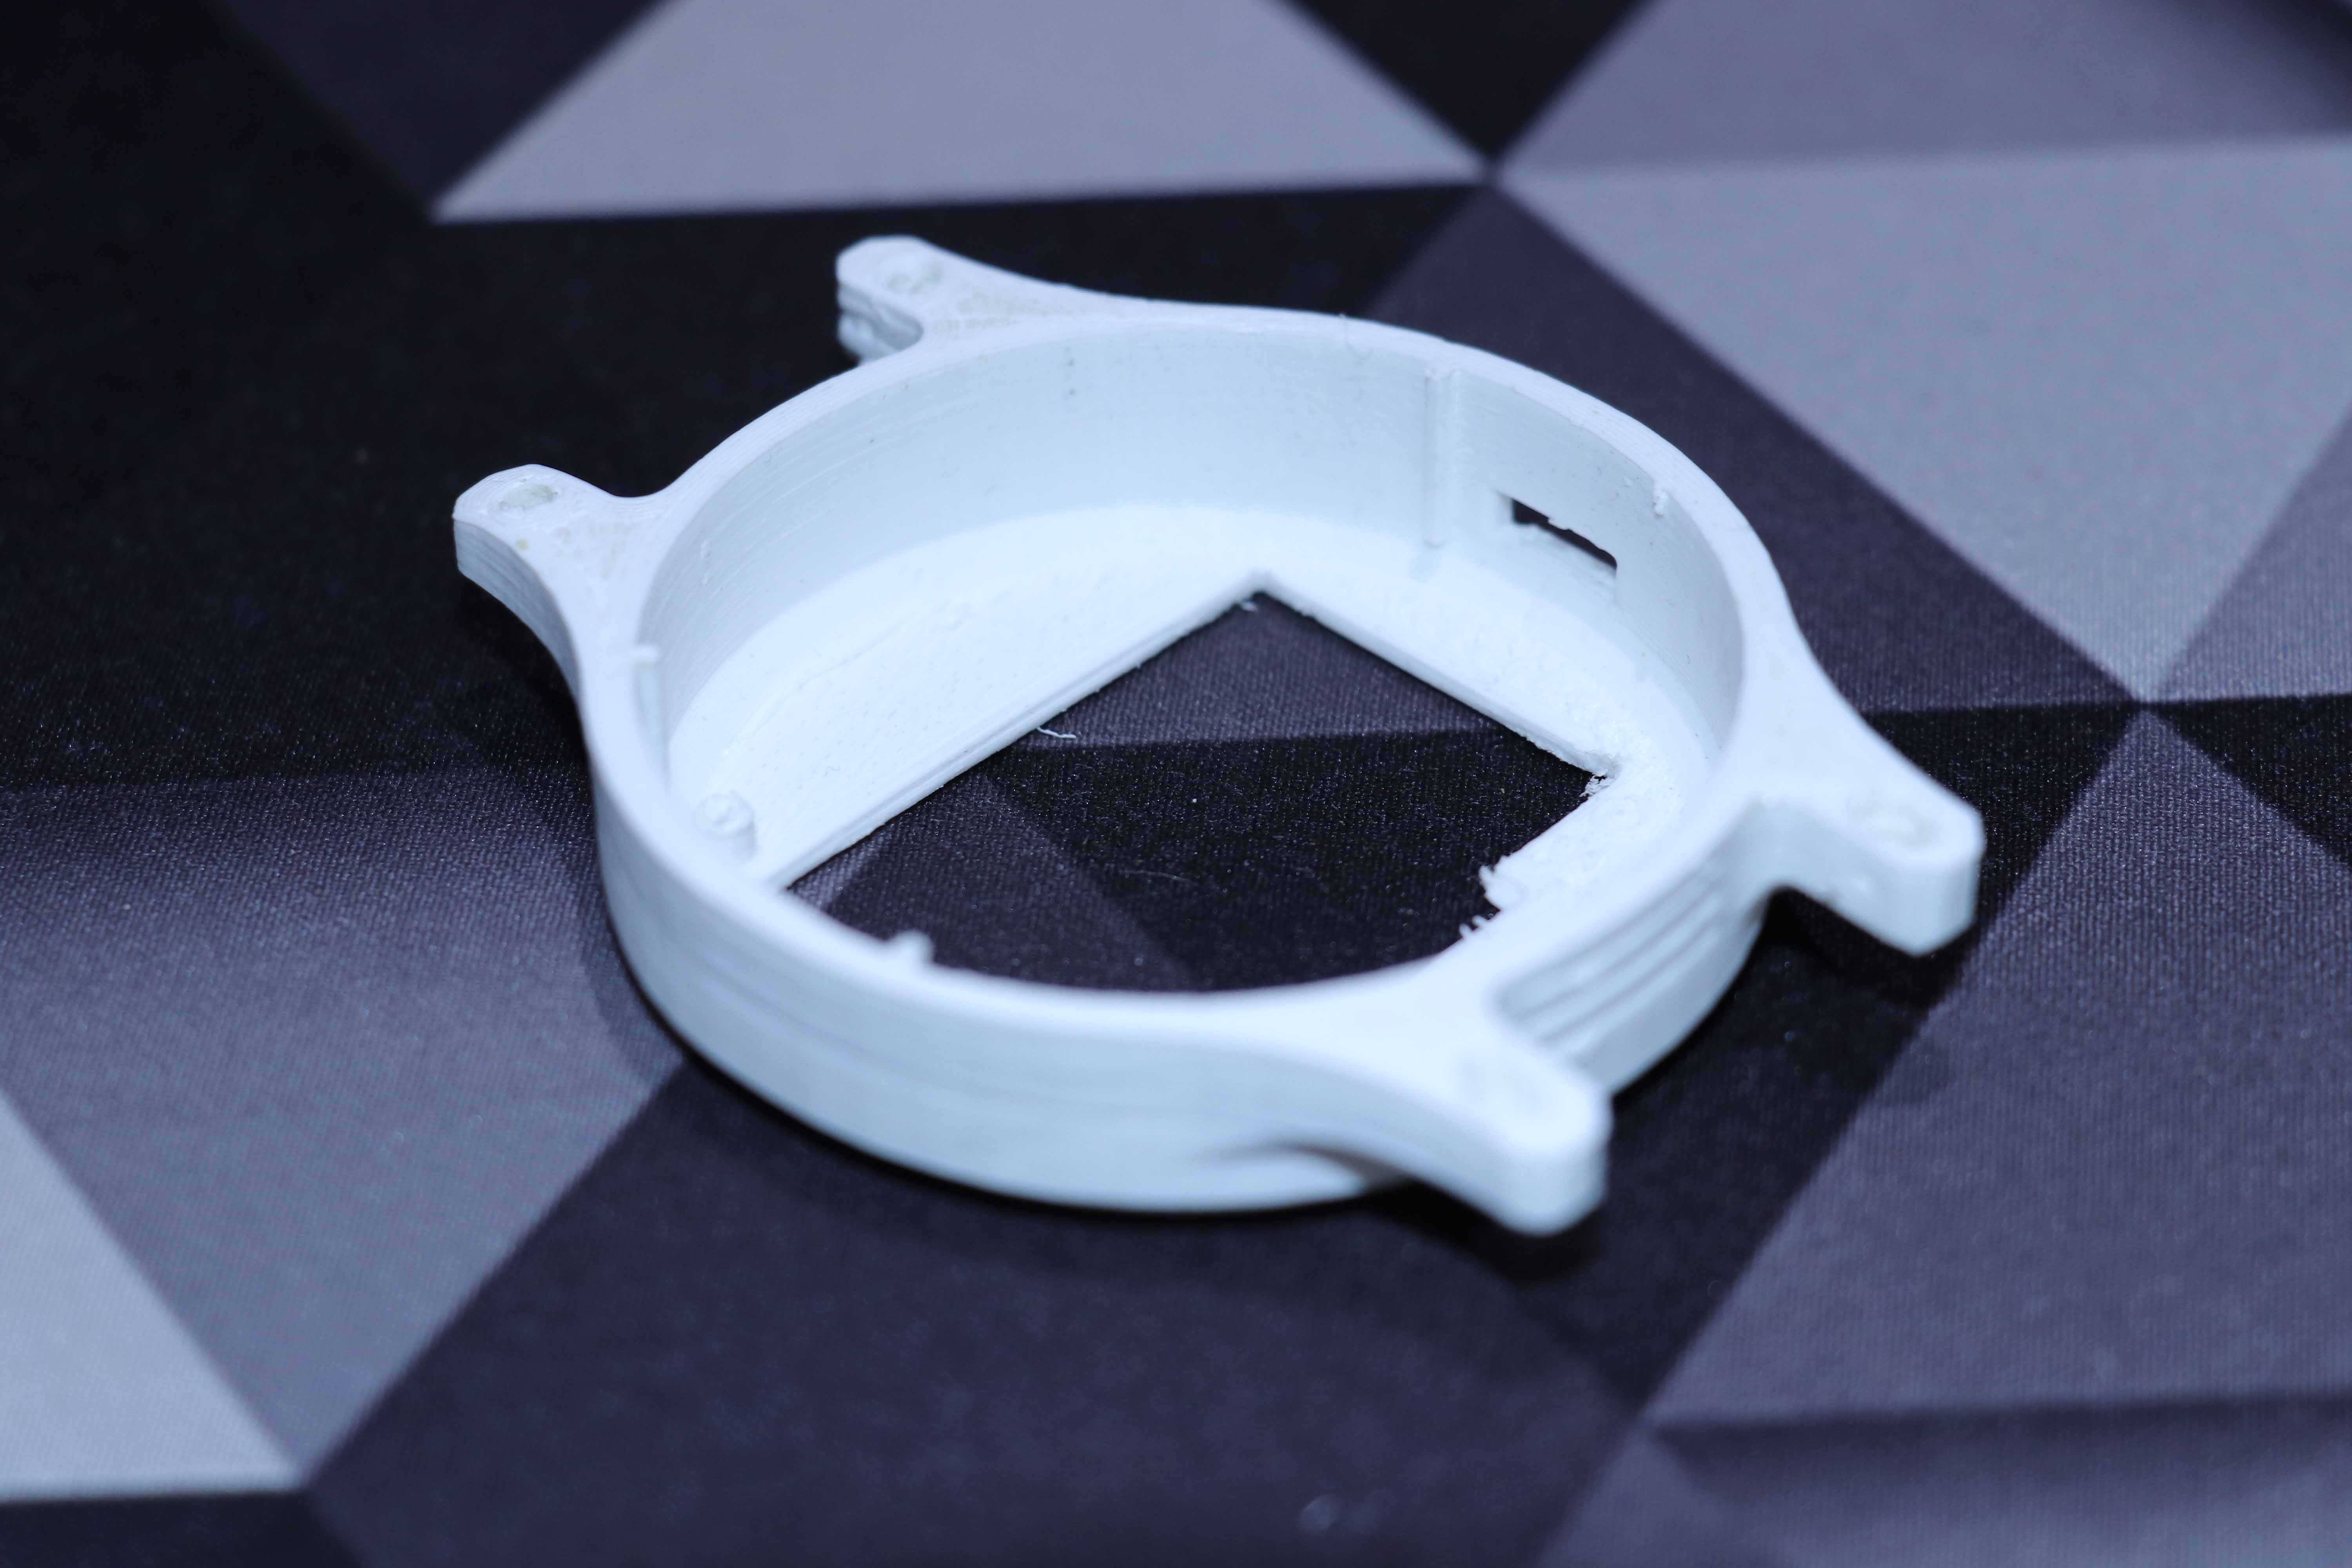
\includegraphics[width=\linewidth]{body_main_v2_back}
		\caption{نمای پشت}
		%\label{fig:oled_image}
	\end{subfigure}
	\begin{subfigure}{0.44\textwidth}
		\centering
		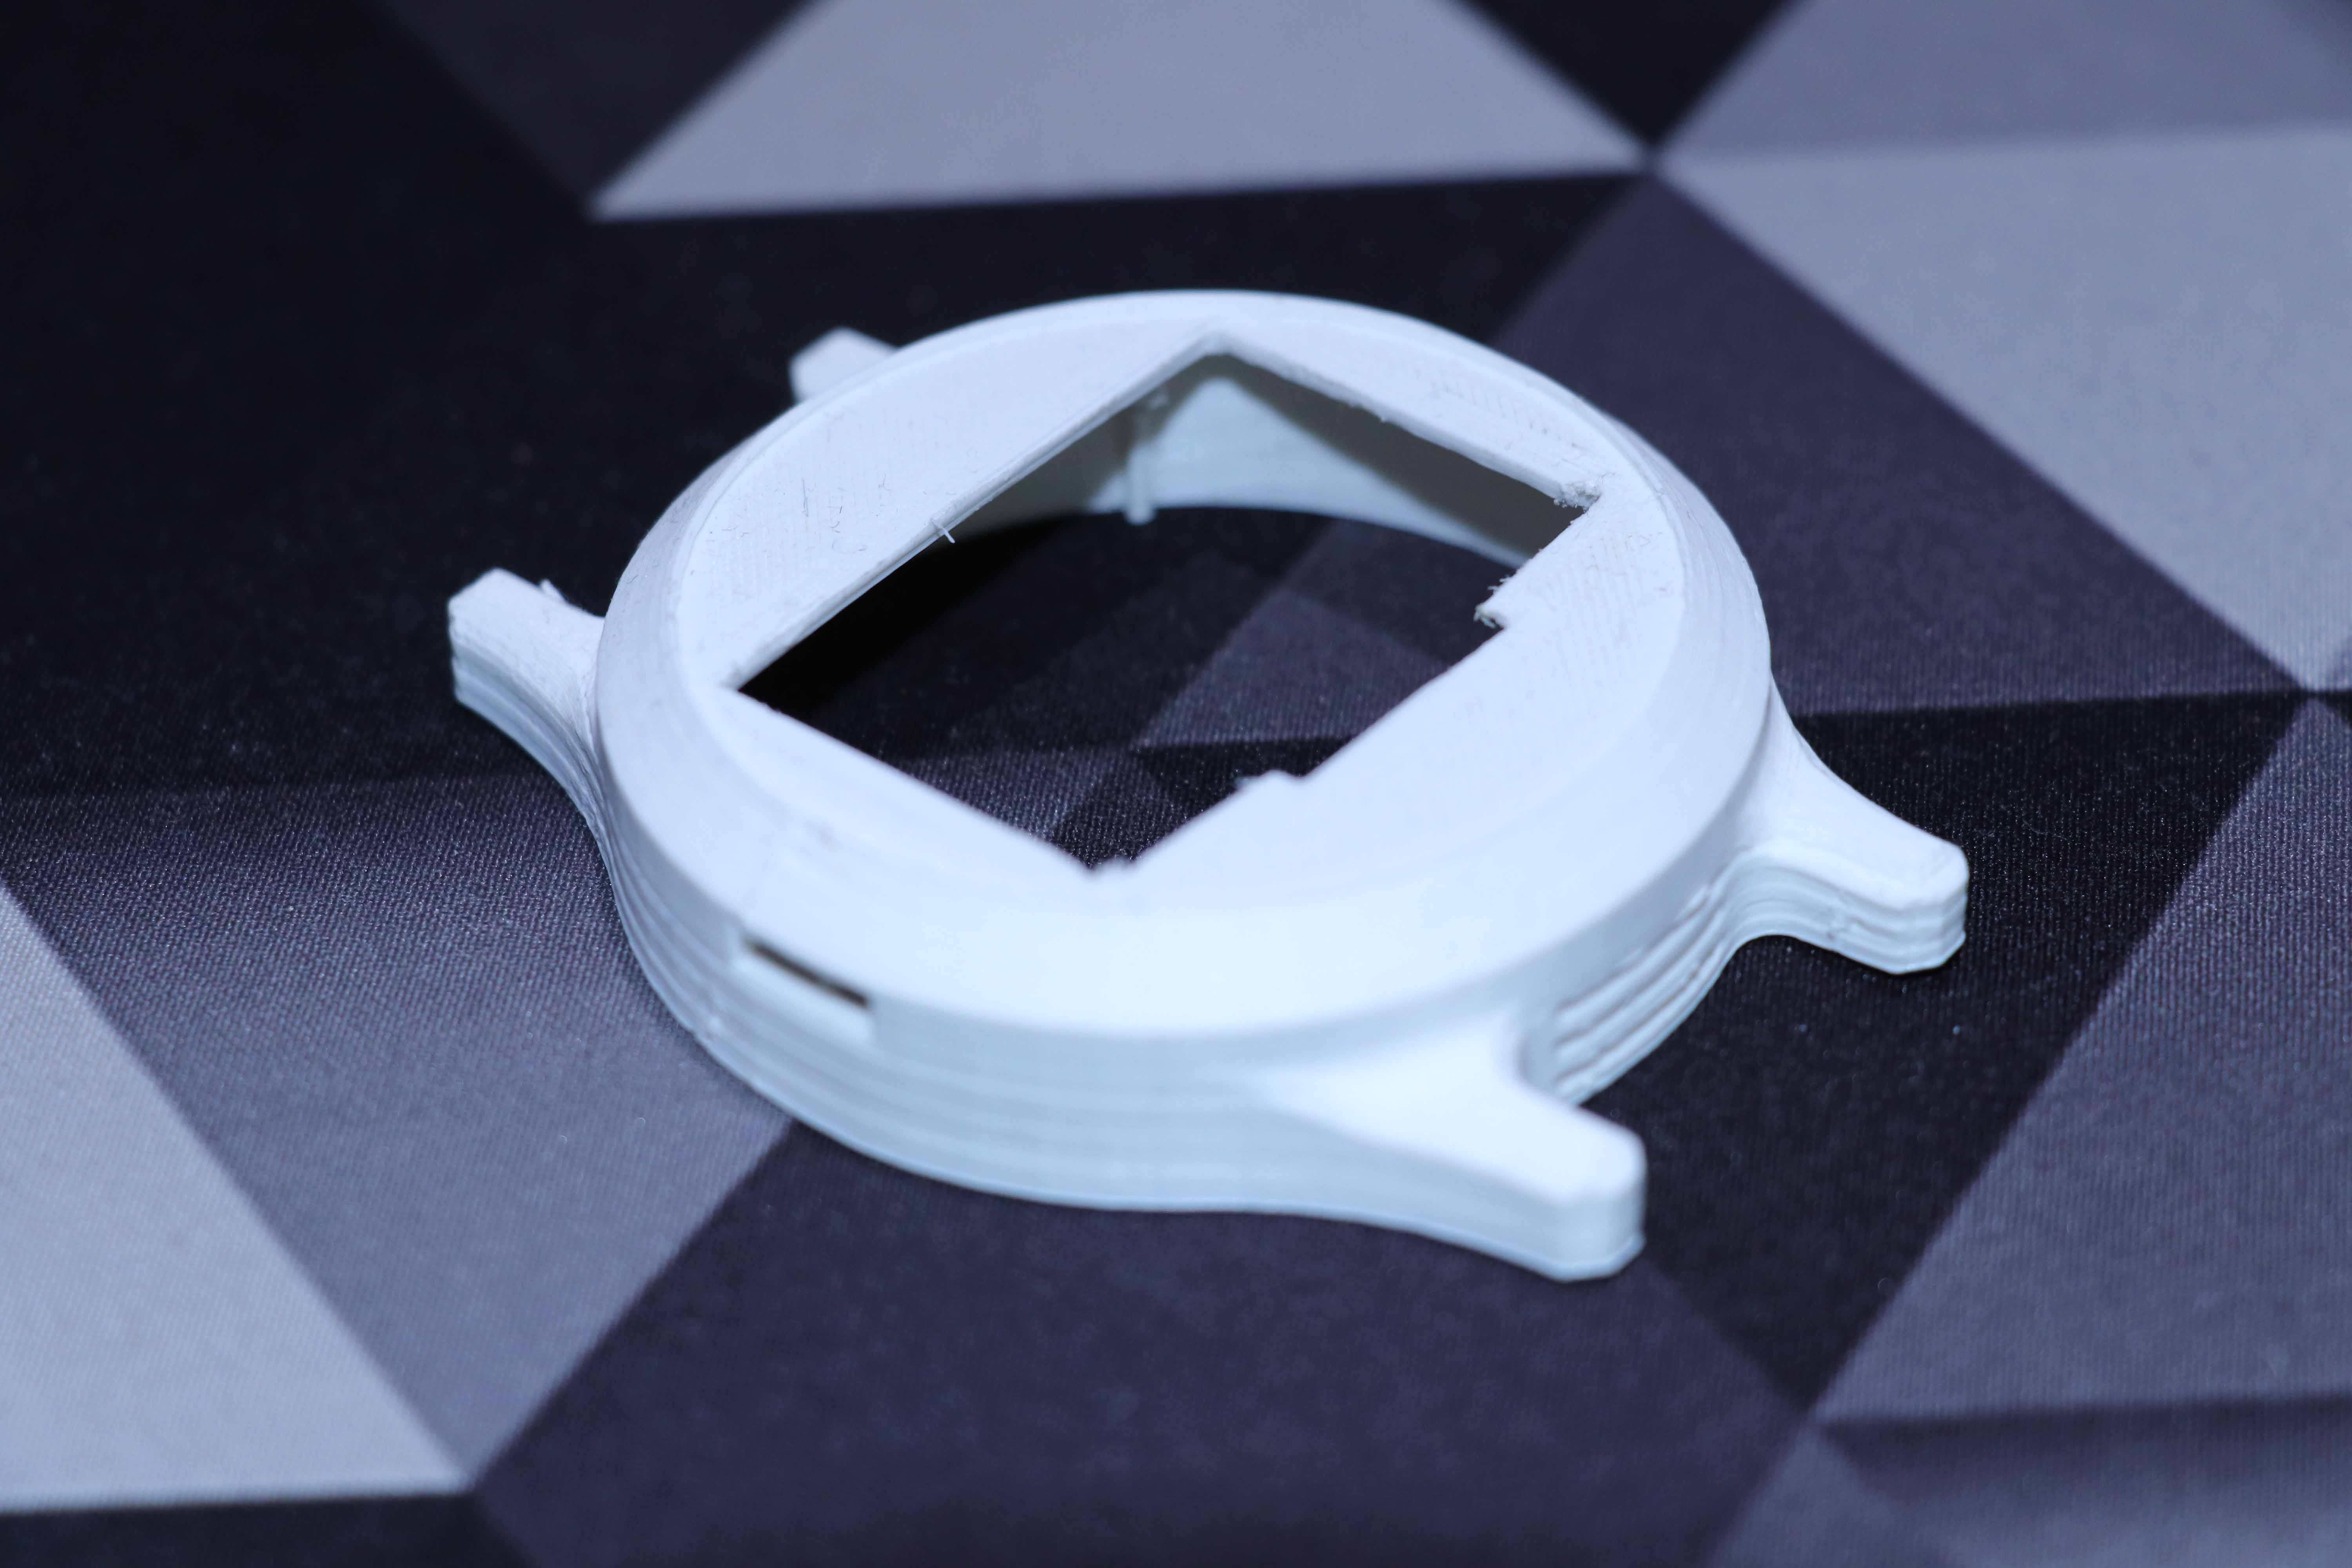
\includegraphics[width=\linewidth]{body_main_v2_front}
		\caption{نمای روبرو}
		%\label{fig:oled_real}
	\end{subfigure}
	\caption{تصاویر بدنه‌ی اصلی نسخه‌ی دوم}
	\label{fig:body-v2}
\end{figure}

این نسخه ایراداتی داشت، از جمله اینکه قسمت مربوط به محل اتصال بند بیش از حد بزرگ بود از زیبایی بصری می‌کاهید. بعد از برطرف نمودن ایرادات این نسخه، نسخه‌ی سوم به چاپ رسید که شکل ؟ آن را نشان می‌دهد.

\begin{figure}[h]
	\centering
	\begin{subfigure}{0.44\textwidth}
		\centering
		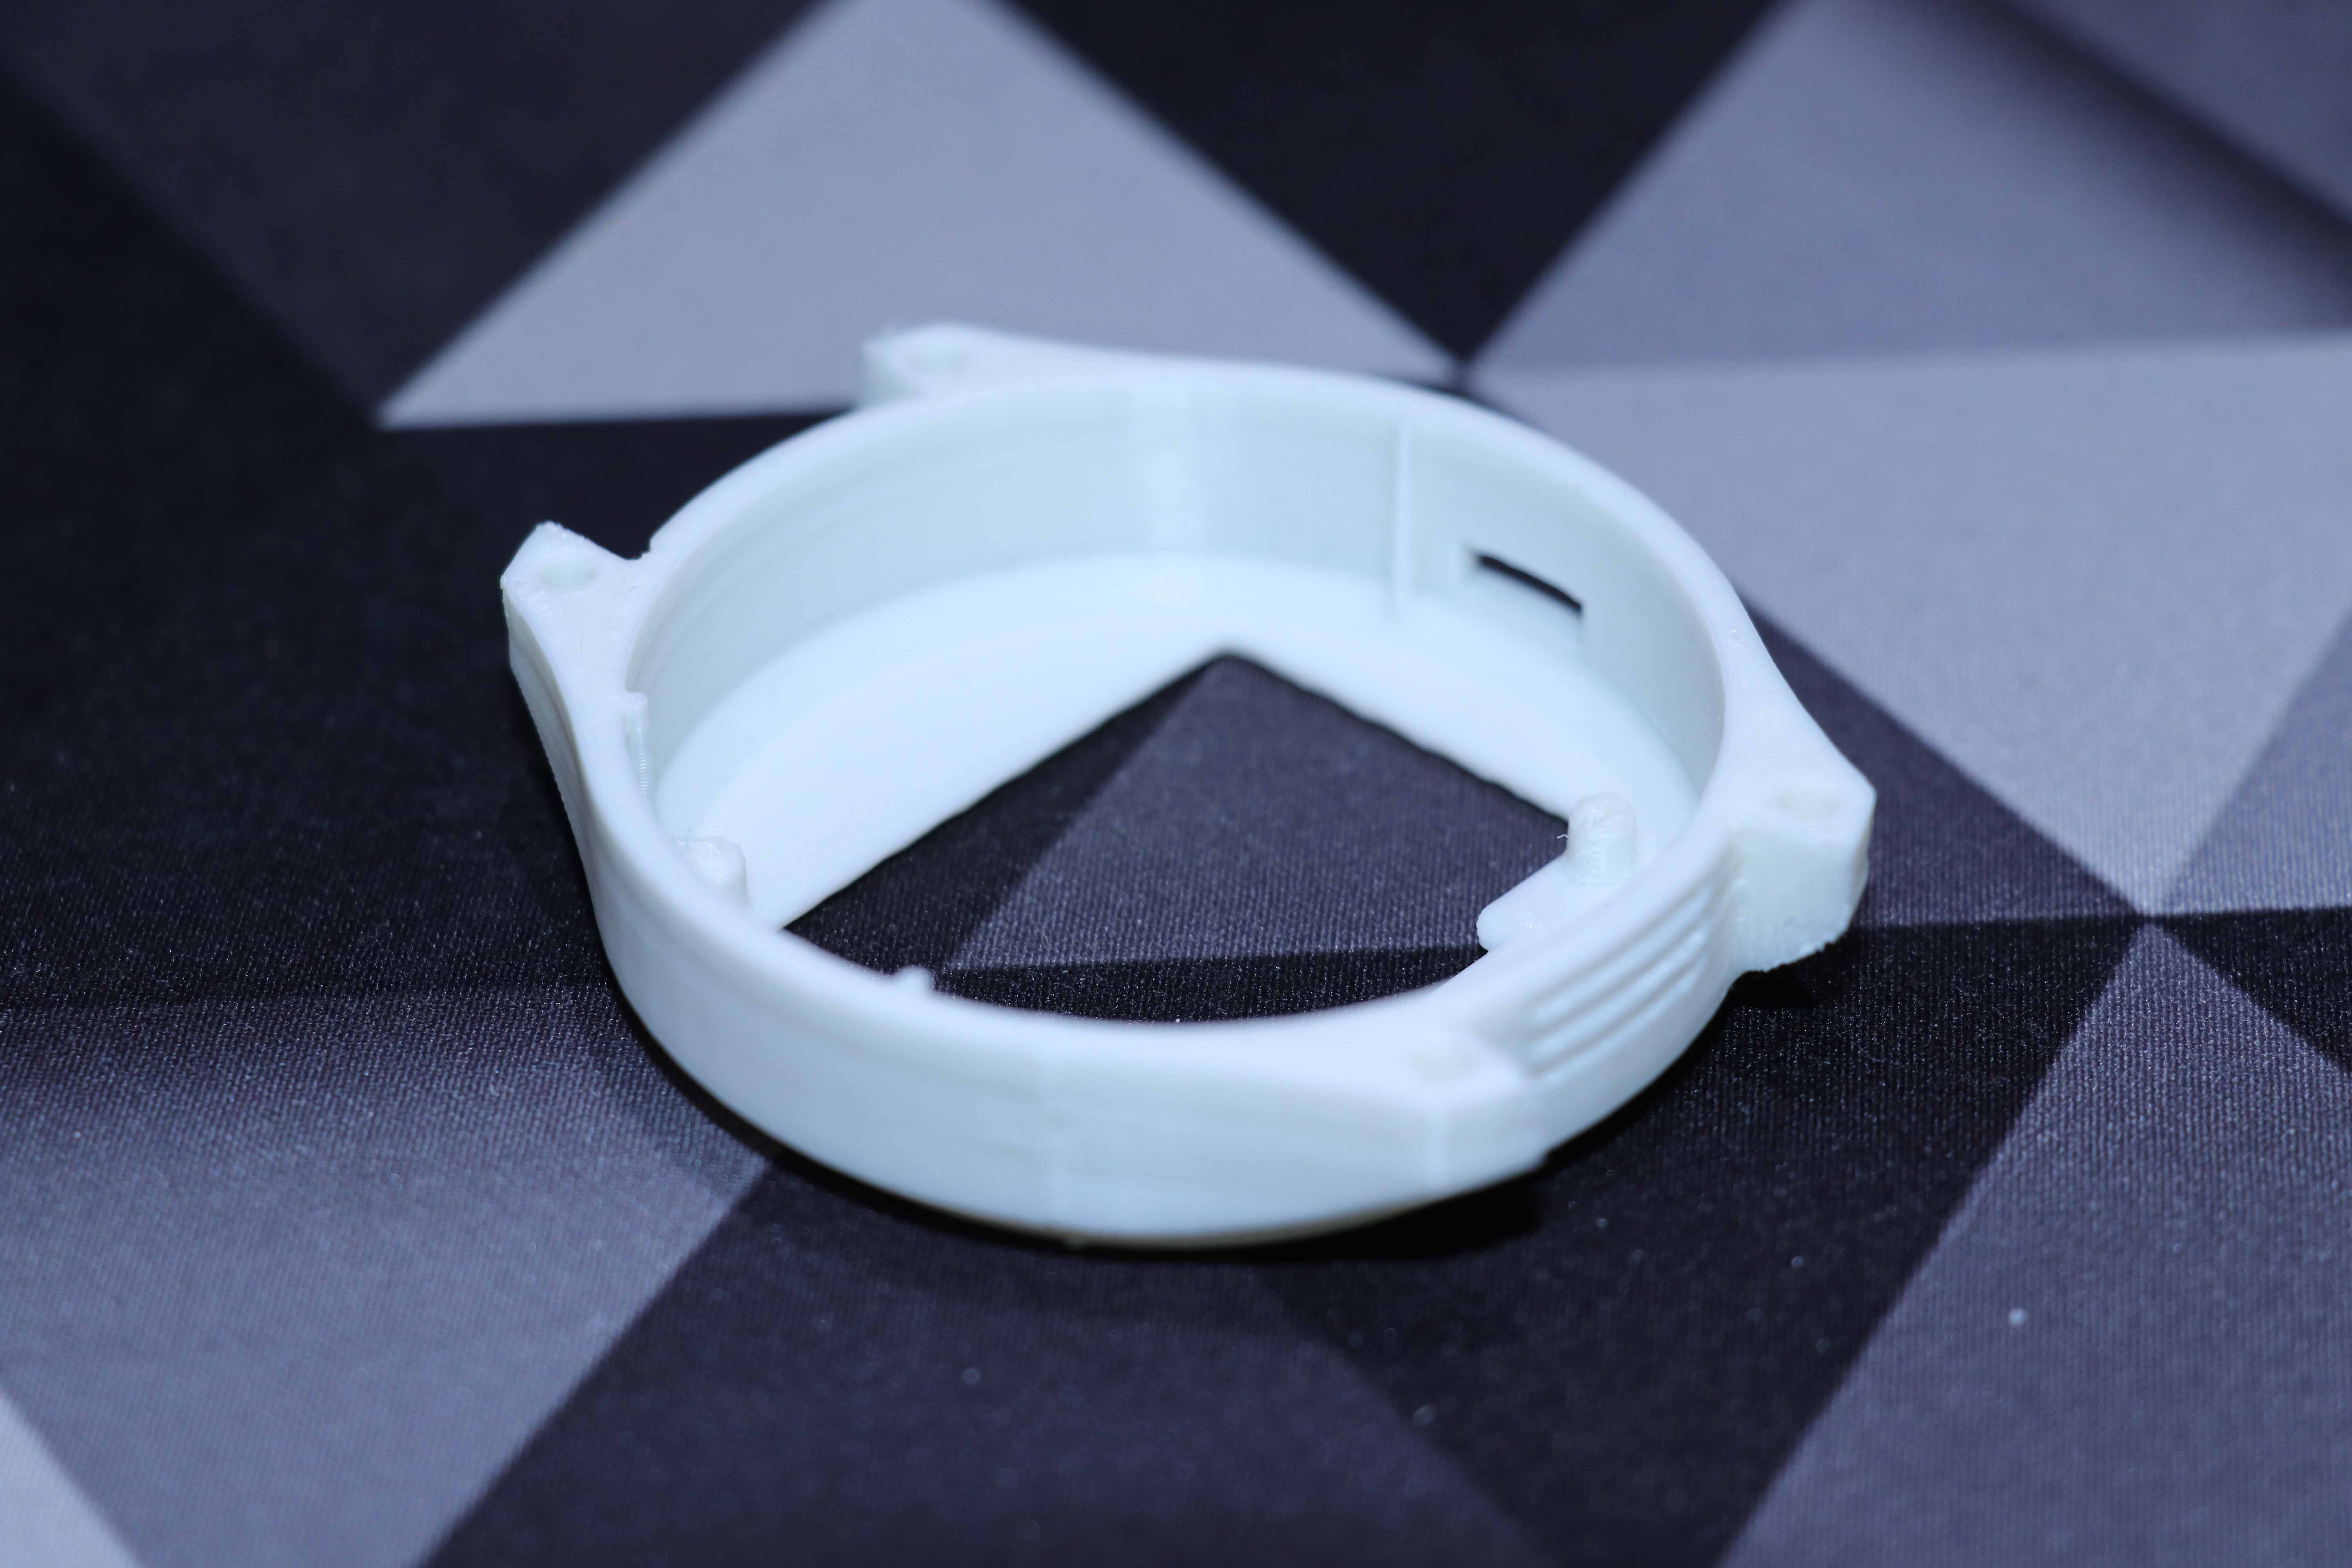
\includegraphics[width=\linewidth]{body_main_v3_back}
		\caption{نمای پشت}
		%\label{fig:oled_image}
	\end{subfigure}
	\begin{subfigure}{0.44\textwidth}
		\centering
		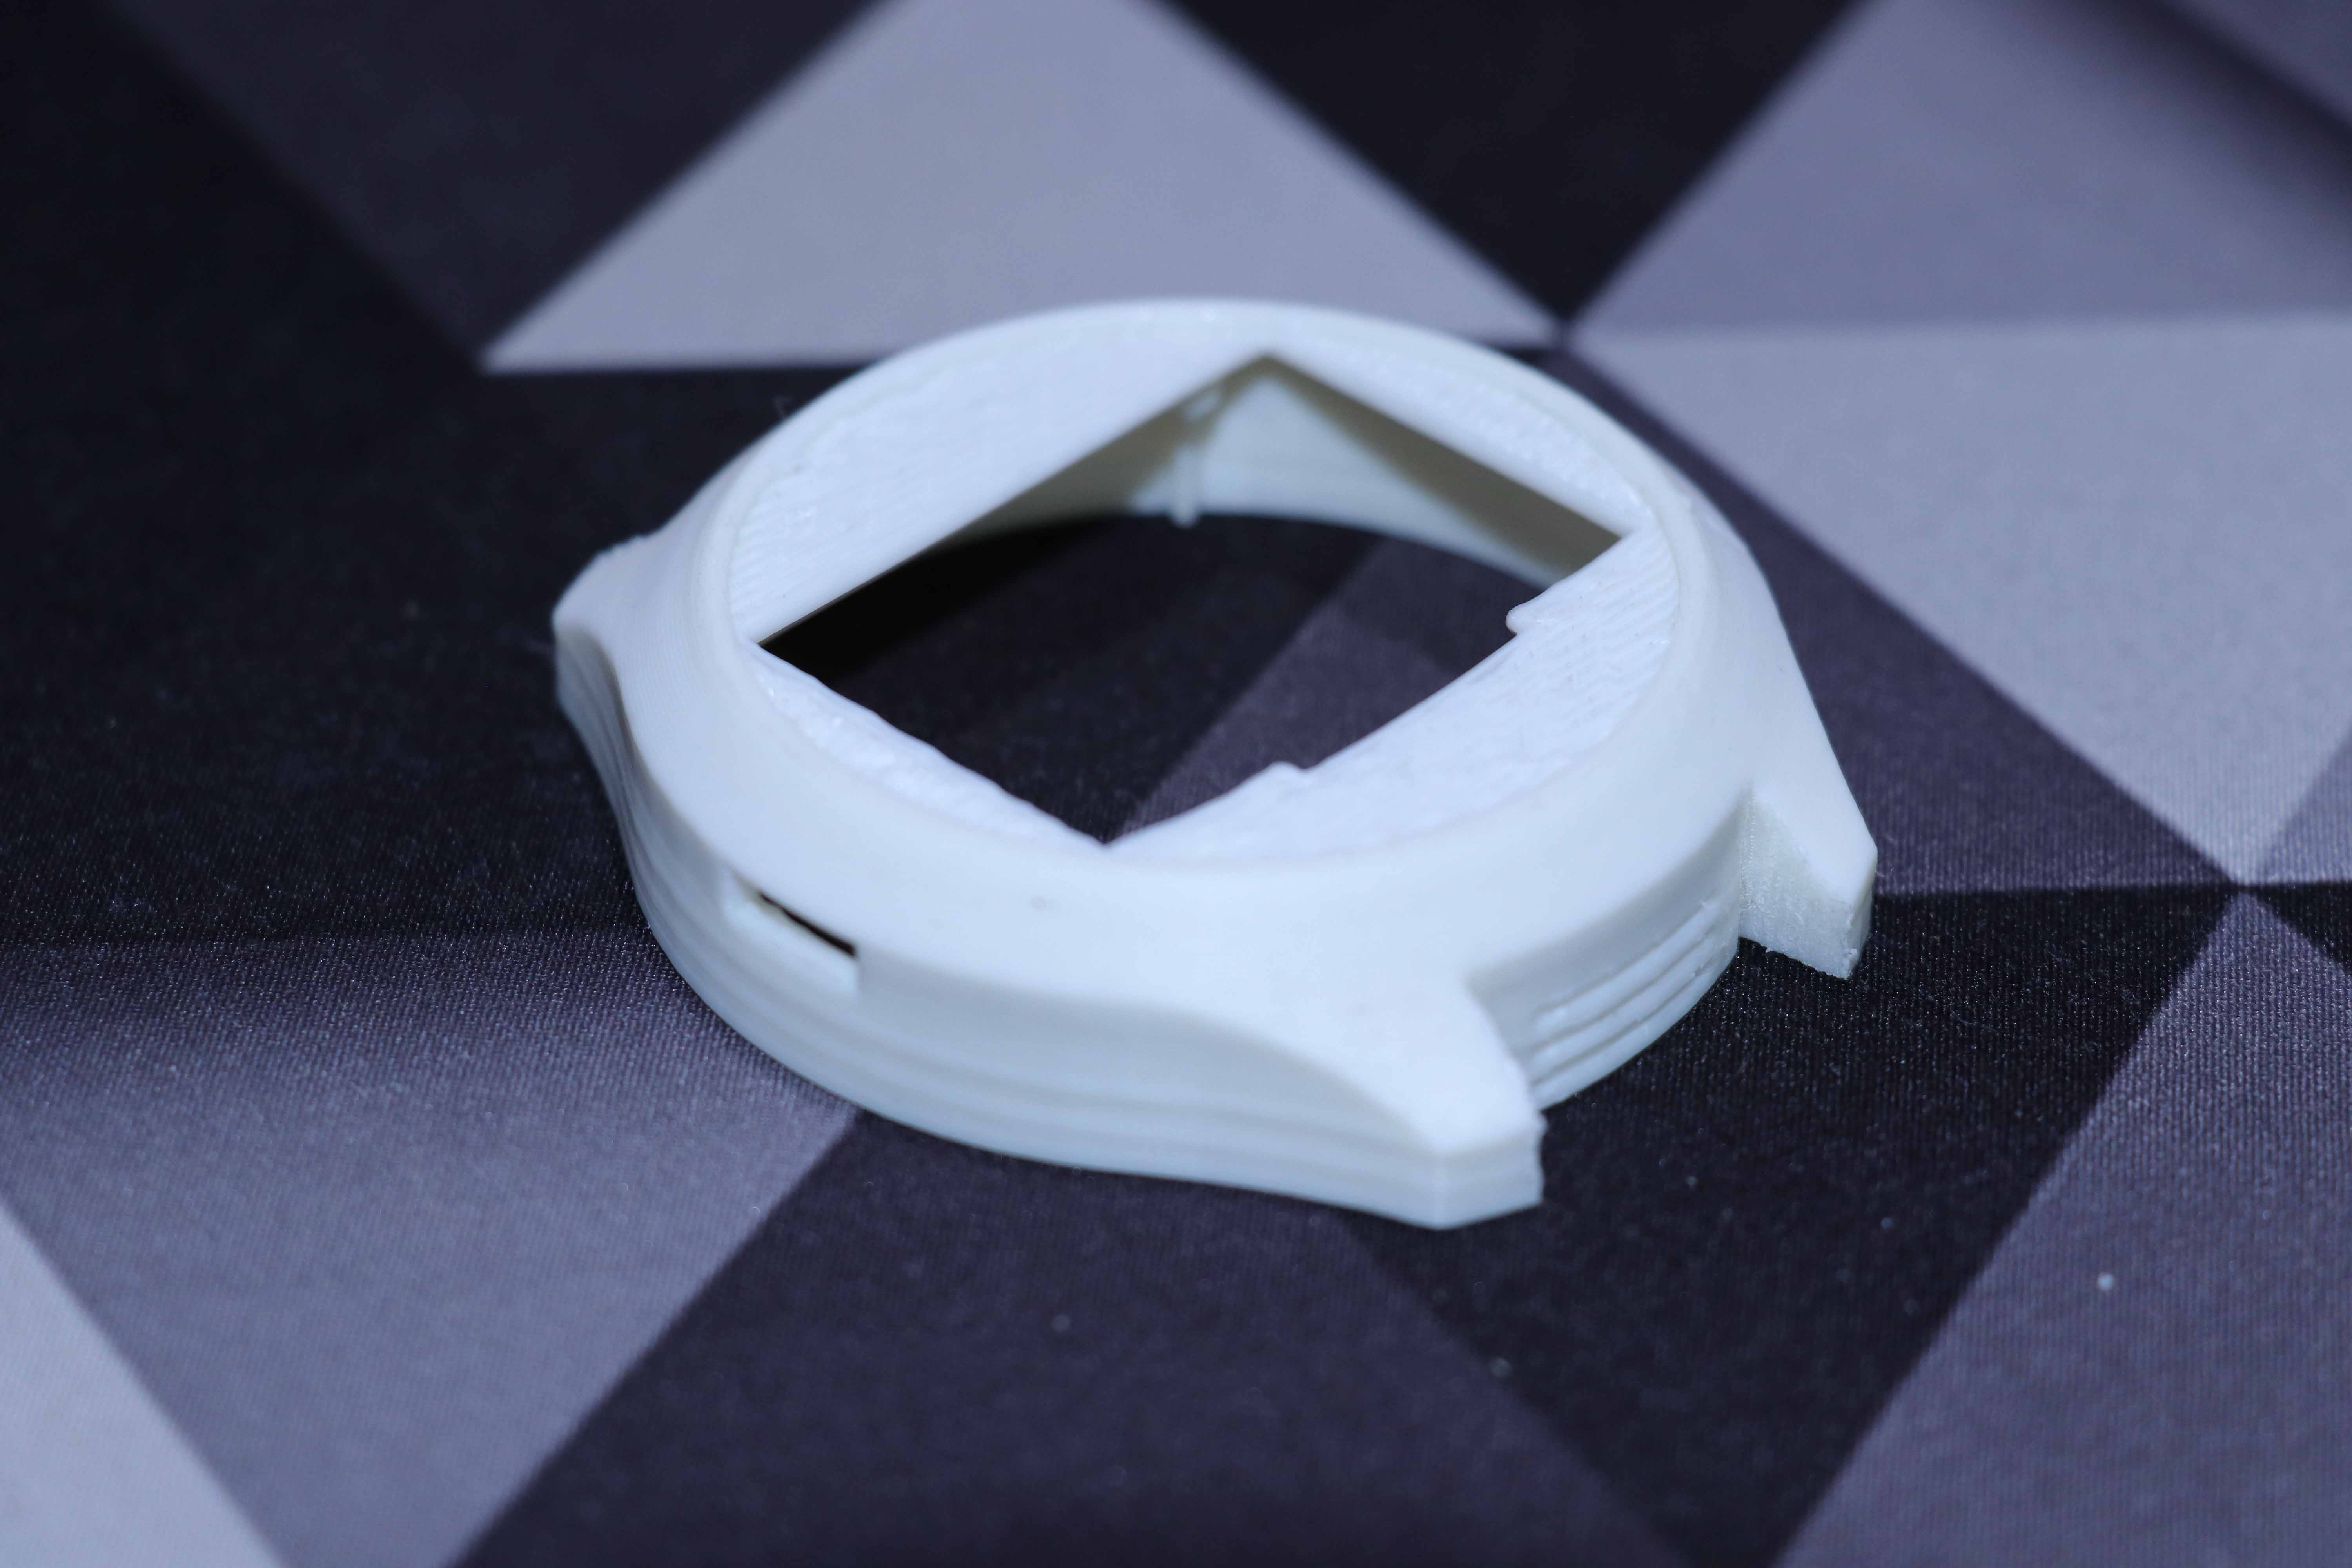
\includegraphics[width=\linewidth]{body_main_v3_front}
		\caption{نمای روبرو}
		%\label{fig:oled_real}
	\end{subfigure}
	\caption{تصاویر بدنه‌ی اصلی نسخه‌ی سوم}
	\label{fig:body-v3}
\end{figure}

این نسخه تقریبا تمام شرایط فوق را ارضا می‌کرد. جانمایی حسگر \lr{PPG} تنها موردی بود که باید انجام میشد. بعد از افزودن این قسمت، نسخه‌ی چهارم و نهایی آماده شد.

\subsection{نسخه نهایی}

شروط بحث شده در بالا را برای نسخه‌ی نهایی بررسی می‌کنیم.
\begin{enumerate}
	\item محل نصب صفحه نمایش:\\
	از سمت بیرون یک مستطیل خالی شده است که تا صفحه نمایش در آن قرار گیرد. از داخل هم سه استوانه منطبق بر سه سوراخ صفحه نمایش وجود دارد تا آن را در جای خود نگه دارد. اگر به تصویر صفحه نمایش (شکل \ref{fig:oled_image}) دقت کنید، پایین آن زائده‌ای برای اتصال سیم‌های فلت به صفحه نمایش قرار دارد. این زائده به شکل یک برش مستطیلی کوچک از صفحه‌ی فوقانی بدنه جدا شده است. شکل \ref{fig:body-oled} این قسمت ها را به خوبی نشان می‌دهد.
	
	\begin{figure}[h]
		\centering
		\begin{subfigure}{0.4\textwidth}
			\centering
			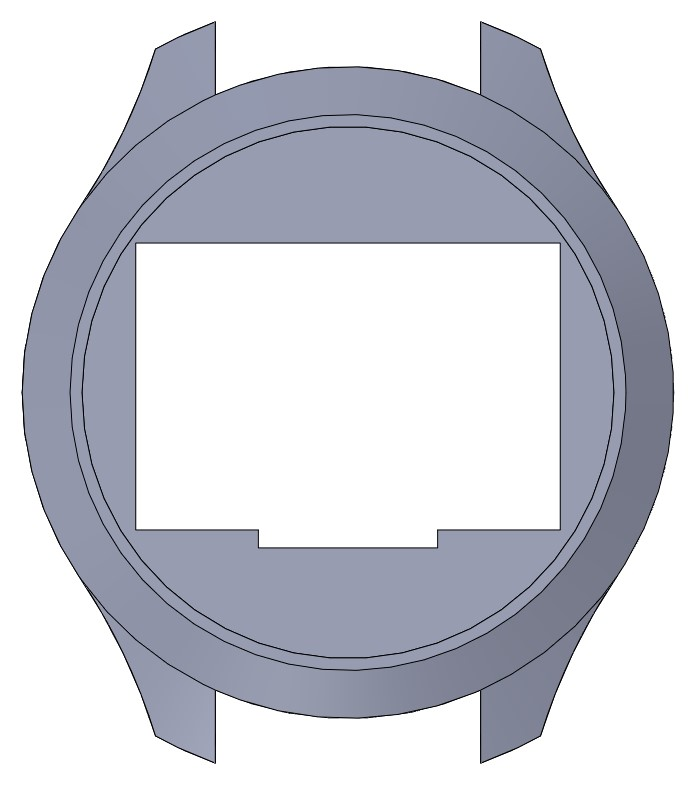
\includegraphics[width=0.78\linewidth]{body_oled}
			\caption{نمای درونی}
			%\label{fig:oled_image}
		\end{subfigure}
		\begin{subfigure}{0.45\textwidth}
			\centering
			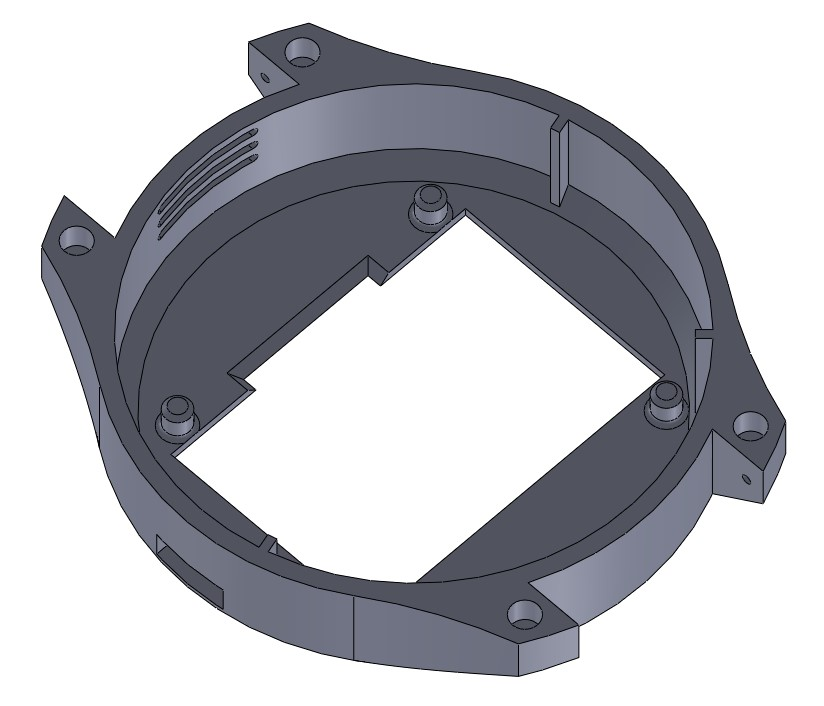
\includegraphics[width=\linewidth]{body_oled2}
			\caption{نمای بیرونی}
			%\label{fig:oled_real}
		\end{subfigure}
		\caption{تصاویر محل نصب صفحه نمایش در بدنه}
		\label{fig:body-oled}
	\end{figure}
	
	\item  جانمایی \pcbf و جلوگیری از چرخش آن:
	بر روی \pcbf سه شیار کوچک وجود دارد. متناظر با آن روی بدنه نیز سه زائده با همان ابعاد تعبیه شده است. این سه زائده مانع چرخش \pcbf در جای خود می‌شوند. تصویر این نگه‌دارنده‌ها در شکل ؟ قابل مشاهده است.
	
	\begin{figure}[h]
		\centering
		\begin{subfigure}{0.4\textwidth}
			\centering
			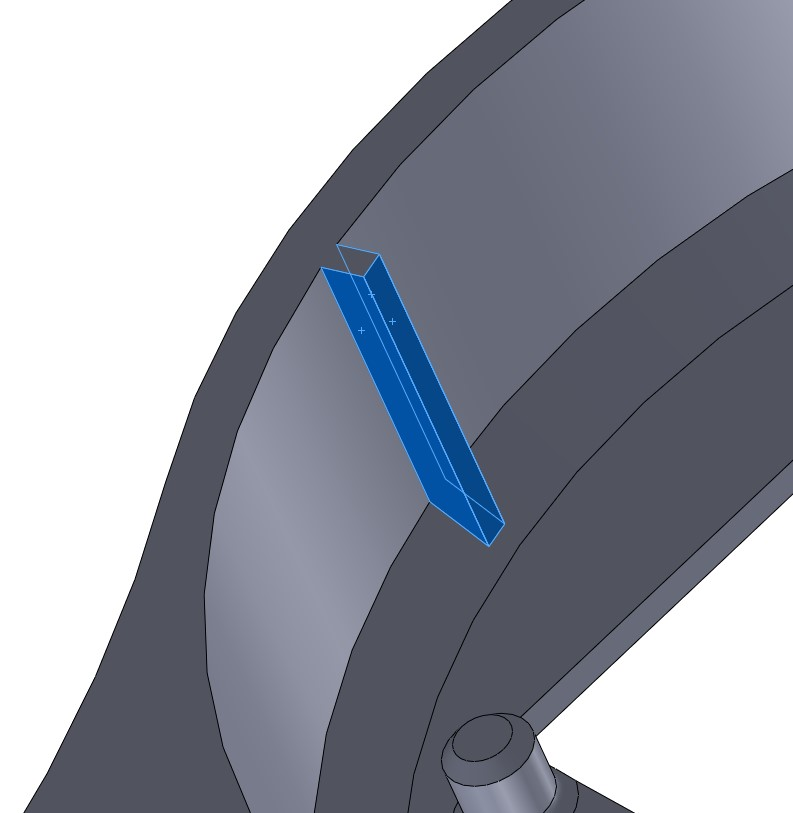
\includegraphics[width=\linewidth]{body_pcb2}
			\caption{نمای درونی}
			%\label{fig:oled_image}
		\end{subfigure}
		\begin{subfigure}{0.45\textwidth}
			\centering
			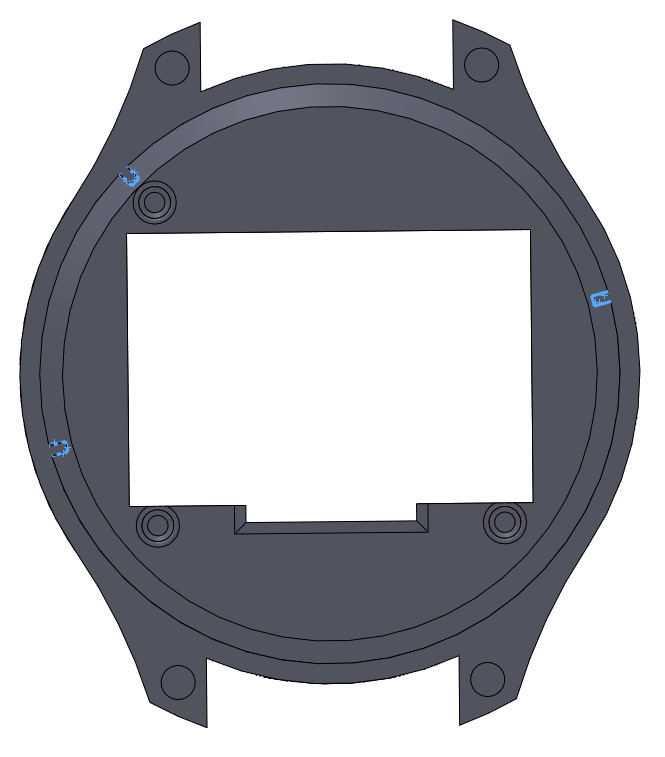
\includegraphics[width=\linewidth]{body_pcb}
			\caption{نمای بیرونی}
			\label{fig:body-pcb-out}
		\end{subfigure}
		\caption{تصاویر محل نصب \pcbf در بدنه}
		\label{fig:body-pcb}
	\end{figure}
	
	\item محل اتصال کابل \lr{USB}:
	بر سطح جانبی بدنه یک سوراخ مستطیل شکل به ابعاد کانکتور \lr{micro USB} تعبیه شده است. شکل \ref{fig:body-usb} محل آن روی بدنه را نمایش می‌دهد.

	\begin{figure}[h]
		\centering
		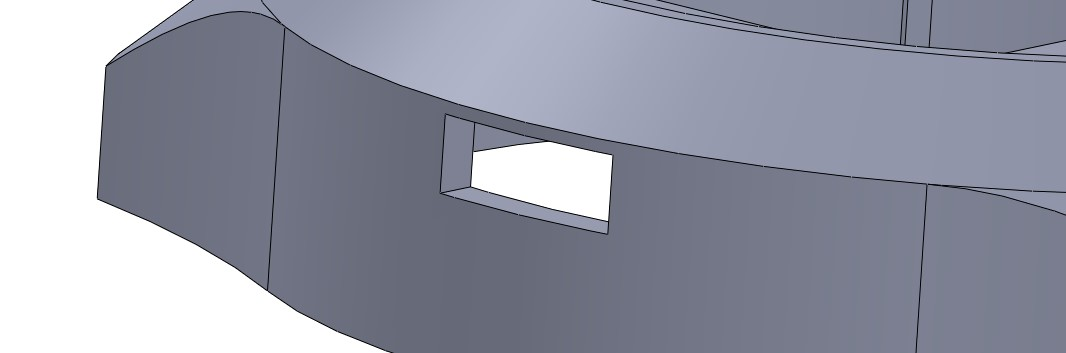
\includegraphics[width=0.9\linewidth]{body_usb}
		\caption{تصویر محل اتصال \lr{USB} در بدنه}
		\label{fig:body-usb}
	\end{figure}
	
	\item محل عبور هوا:
	در نزدیکی قطعات مدار شارژ سه شیار برای عبور هوا وجود دارد تا قطعات داخلی به علت بالا رفتن دما آسیب نبینند. این شیارها در شکل \ref{fig:body-air} قابل مشاهده‌اند.
	
	\begin{figure}[h]
		\centering
		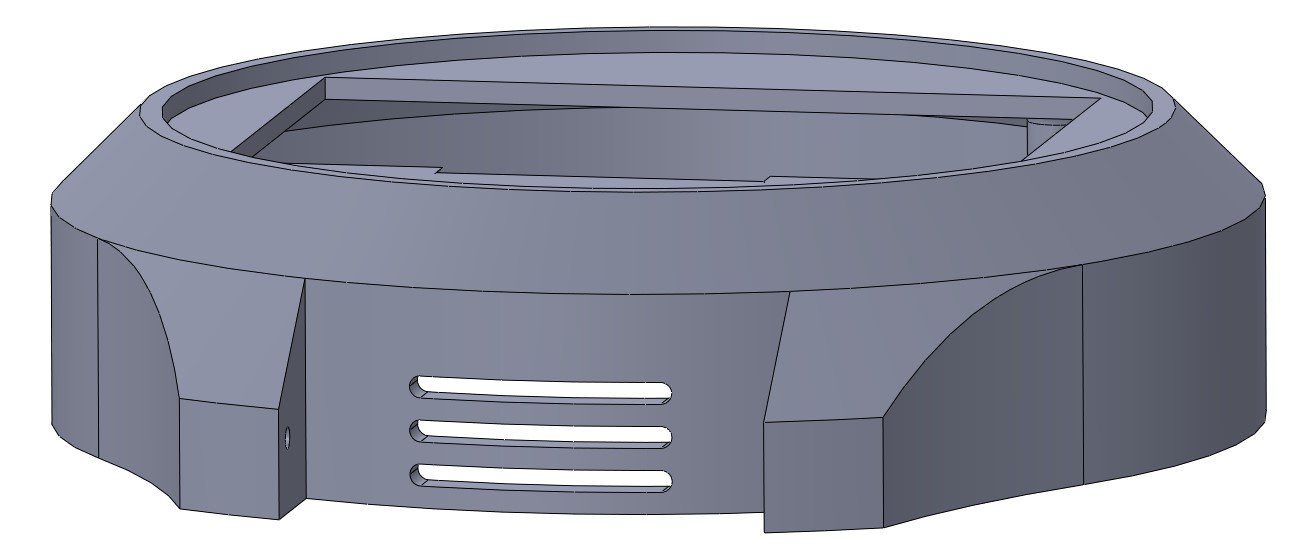
\includegraphics[width=0.9\linewidth]{body_air}
		\caption{تصویر شیارهای عبور هوا}
		\label{fig:body-air}
	\end{figure}

	\item محل اتصال بند
	بندهای موردنظر برای این ساعت مربوط به ساعت هوشمند \lr{Haylou} است. این بندها از جنس پلاستیک هستند. برای اتصال بند به بدنه‌ی اصلی چهار بازوی کوچک به بدنه اضافه شده است. داخل آن‌ها سوراخ‌هایی کوچکی موجود است که پین بند در آن‌ها قرار گیرد. تصویر این بازوها و محل نصب پین را شکل \ref{fig:body-band} مشاهده می‌کنید.
	
	\begin{figure}[h]
		\centering
		\begin{subfigure}{0.4\textwidth}
			\centering
			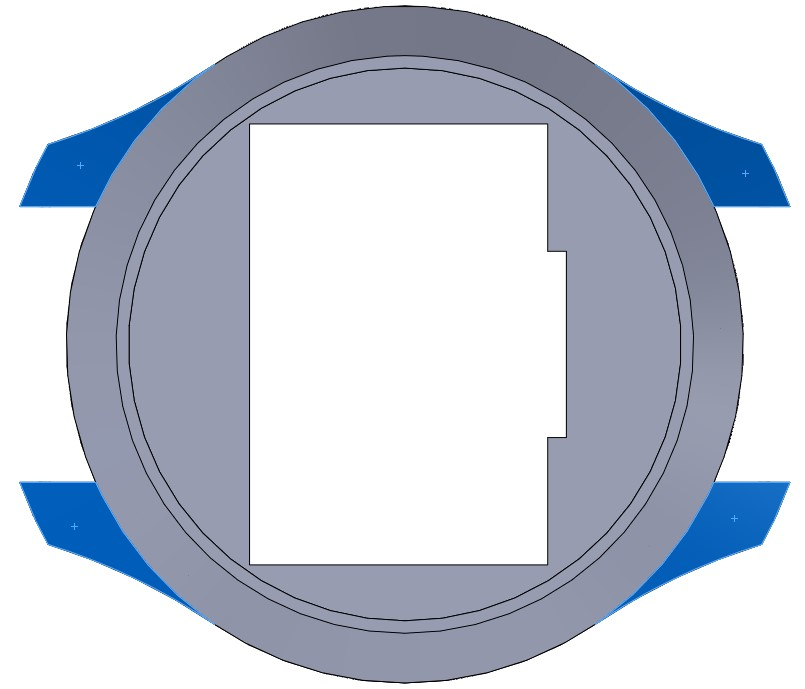
\includegraphics[width=\linewidth]{body_band}
			\caption{چهار بازو برای اتصال بند}
			%\label{fig:oled_image}
		\end{subfigure}
		\begin{subfigure}{0.3\textwidth}
			\centering
			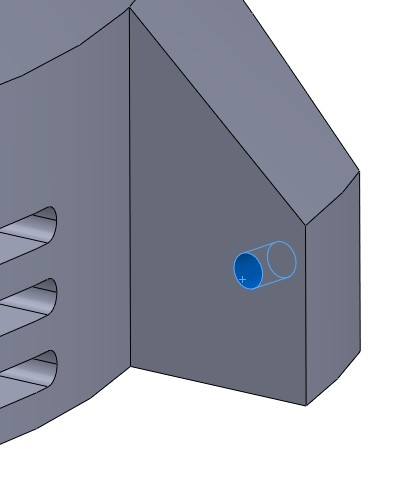
\includegraphics[width=\linewidth]{body_band2}
			\caption{سوراخ های نصب پین}
			%\label{fig:oled_real}
		\end{subfigure}
		\caption{تصاویر محل نصب بند}
		\label{fig:body-band}
	\end{figure}

	\item زیبایی بصری: جای تردید نیست که این طرح زیبا است :)
	\item ابعاد دقیق طرح در بخش‌های بعدی تشریخ خواهد شد؛ اما در مورد تناسب ابعاد، قطر دایره‌ی این ساعت حدود 5 سانتی‌متر است که در مقایسه با ساعت‌های موجود در بازار، مقدار بزرگی نیست و معقول است.
\end{enumerate}

در نهایت تصویر بدنه‌ی اصلی در شکل \ref{fig:body-real} دیده می‌شود. چاپ این نسخه توسط شرکت \lr{PCBWay}\cite{PCBWay} به رایگان انجام شده است. جنس بدنه از رزین است که باعث می‌شود شفاف باشد و داخل آن دیده شود.

	\begin{figure}[h]
		\centering
		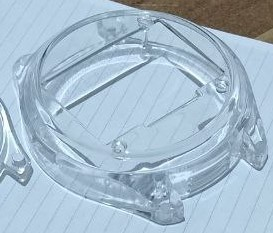
\includegraphics[width=0.5\linewidth]{body_real2}
		\caption{تصویر چاپ شده‌ی نسخه‌ی نهایی بدنه از جنس رزین و شفاف}
		\label{fig:body-real}
	\end{figure}

\section{دریچه‌ی پشتی}
دریچه‌ی پشتی وظیفه دارد تا بر پشت بدنه‌ی اصلی نصب شود و قطعات و تجهیزات داخل ساعت را محافظت کند. از طرفی محل نصب حسگر \lr{PPG} نیز هست. این دو وظیفه را شرح می‌دهیم.

\begin{enumerate}
	\item اتصال به بدنه‌ی اصلی:
	برای اتصال به بدنه‌ی اصلی، چهار استوانه‌ی کوچک بر روی دریچه طراحی شده ‌است. این استوانه‌ها منطبق بر سوراخ‌های روی بدنه است. این سوراخ‌ها در شکل \ref{fig:body-pcb-out} به خوبی دیده می‌شوند. بدین شکل دریچه به بدنه متصل می‌شود. تصویر دریچه در شکل \ref{fig:body-back2main} نشان داده شده‌است.
	
	\begin{figure}[h]
		\centering
		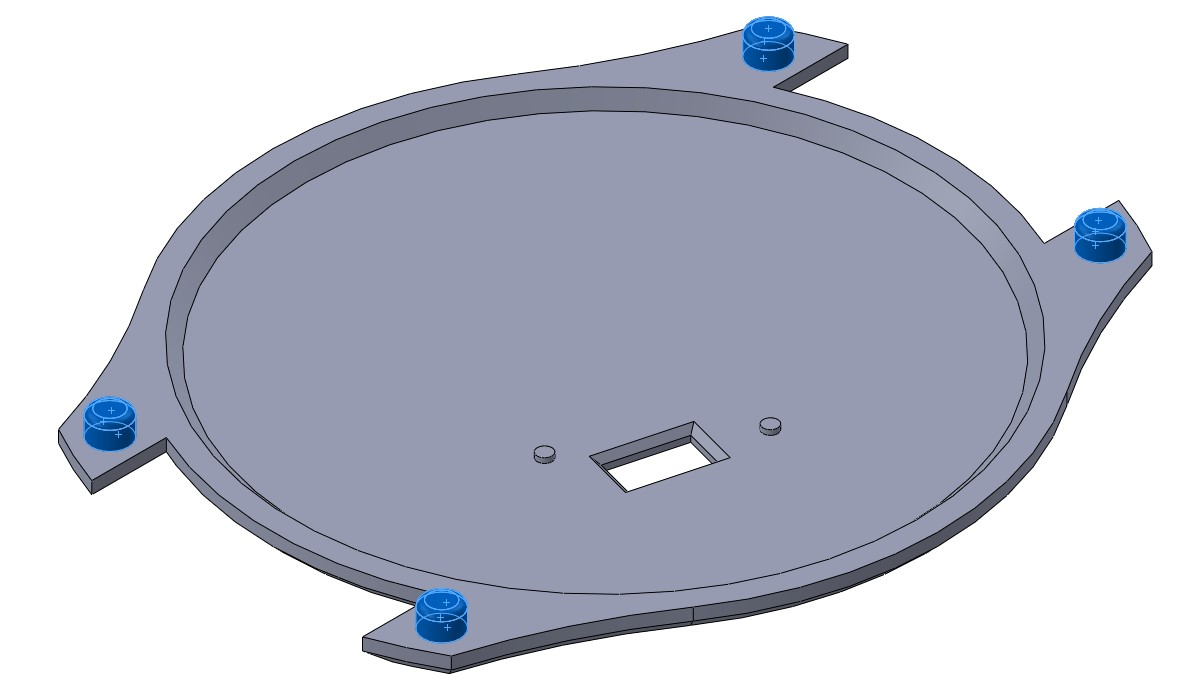
\includegraphics[width=0.7\linewidth]{body_back2main}
		\caption{تصویر استوانه‌های اتصال دریچه به بدنه}
		\label{fig:body-back2main}
	\end{figure}
	
	\item اتصال حسگر \lr{PPG}:
	حسگر باید جایی نصب شود که با پوست تماس مستقیم داشته باشد. لذا بر روی دریچه سوراخ مستطیل شکلی ایجاد شده است تا محل نصب حسگر باشد. دو زائده‌ی کوچک نیز در نزدیکی آن قرار دارد تا منطبق بر سوراخ‌های روی حسگر باشد. این سوراخ‌ها در شکل \ref{fig:ppg_image} قابل مشاهده ‌اند. شکل \ref{fig:body-ppg} محل نصب حسگر را نشان می‌دهد.
	
	\begin{figure}[h]
		\centering
		\begin{subfigure}{0.35\textwidth}
			\centering
			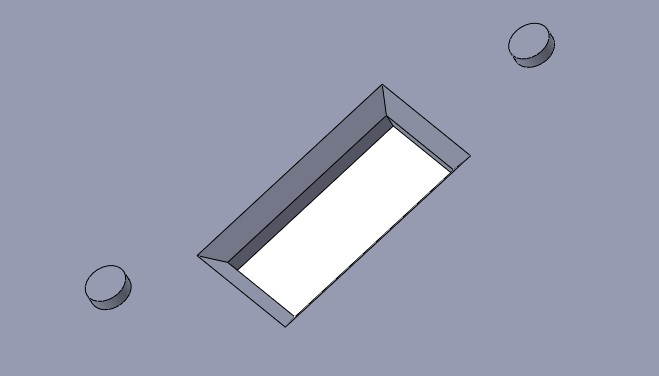
\includegraphics[width=\linewidth]{body_ppg}
			\caption{نمای درونی}
			%\label{fig:oled_image}
		\end{subfigure} 
		\begin{subfigure}{0.45\textwidth}
			\centering
			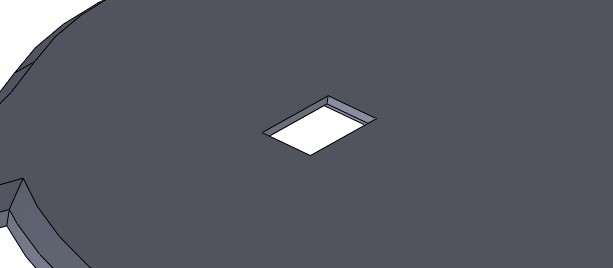
\includegraphics[width=\linewidth]{body_ppg2}
			\caption{نمای بیرونی}
			%\label{fig:oled_real}
		\end{subfigure}
		\caption{تصاویر محل نصب حسگر \lr{PPG}}
		\label{fig:body-ppg}
	\end{figure}

\end{enumerate}

در نهایت تصویر دریچه‌ی پشتی در شکل \ref{fig:body-back-reel} دیده می‌شود. چاپ این نسخه نیز توسط شرکت \lr{PCBWay}\cite{PCBWay} به رایگان انجام شده است. جنس بدنه از رزین است که باعث می‌شود شفاف باشد و داخل آن دیده شود.

	\begin{figure}[h]
		\centering
		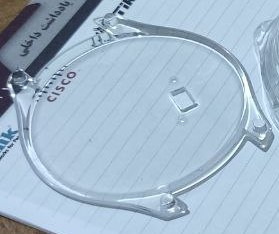
\includegraphics[width=0.5\linewidth]{body_real4}
		\caption{تصویر چاپ شده‌ی نسخه‌ی نهایی دریچه‌ی پشتی از جنس رزین و شفاف}
		\label{fig:body-back-reel}
	\end{figure}

\section{اتصالات}
 تمامی اتصالات مکانیکی در این بخش توضیح داده می‌شود.
 
 \subsection{کلیدهای لمسی}
 باید چهار قطعه سیم به شکل حلقوی سیم پیچی شده و از داخل به بدنه‌ی اصلی چسبانده شود. بدین منظور از سیم‌های وایر رپ\footnote{\lr{Wire wrap}} استفاده شده است. همانطور که در شکل \ref{fig:conn-touch} دیده می‌شود این سیم‌ها به کمک چسب نواری به بدنه‌ی اصلی متصل شده‌اند. کلیدهای لمسی به کمک خاصیت خازنی کار می‌کنند. سر دیگر سیم‌ها به محل اتصال کلیدهای لمسی در شکل \ref{fig:touch_real} لحیم می‌شوند.
 
با توجه به این که می‌توان لایه‌ی نازک فوقانی را به صورت یک دی‌الکتریک برای خازن در نظر گرفت، می‌توان گفت با اینکه کلیدهای پشت صفحه نصب شده‌اند اما باز هم به درستی کار خواهند کرد. 

	\begin{figure}[h]
		\centering
		\begin{subfigure}{0.45\textwidth}
			\centering
			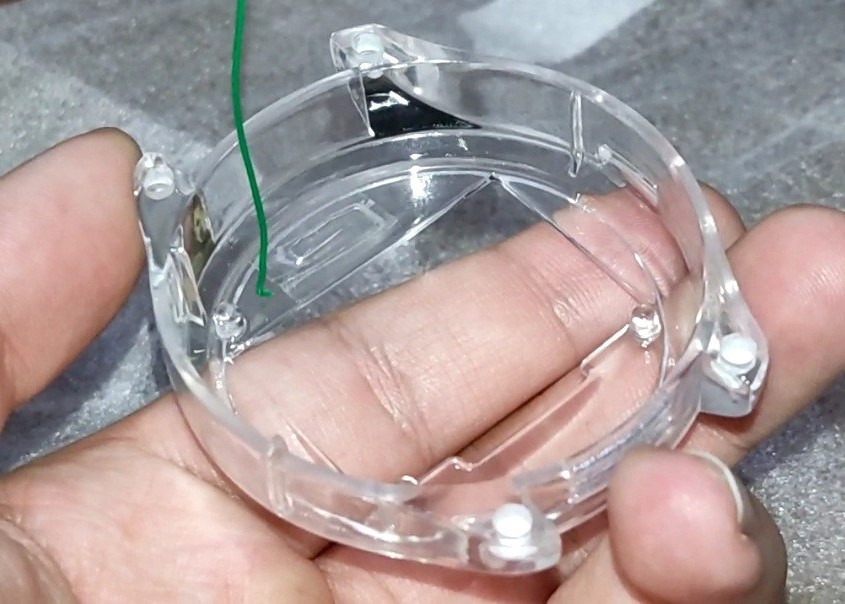
\includegraphics[width=\linewidth]{conn-touch}
			\caption{یک کلید نصب شده بر پشت سطح فوقانی}
			%\label{fig:oled_image}
		\end{subfigure} 
		\begin{subfigure}{0.45\textwidth}
			\centering
			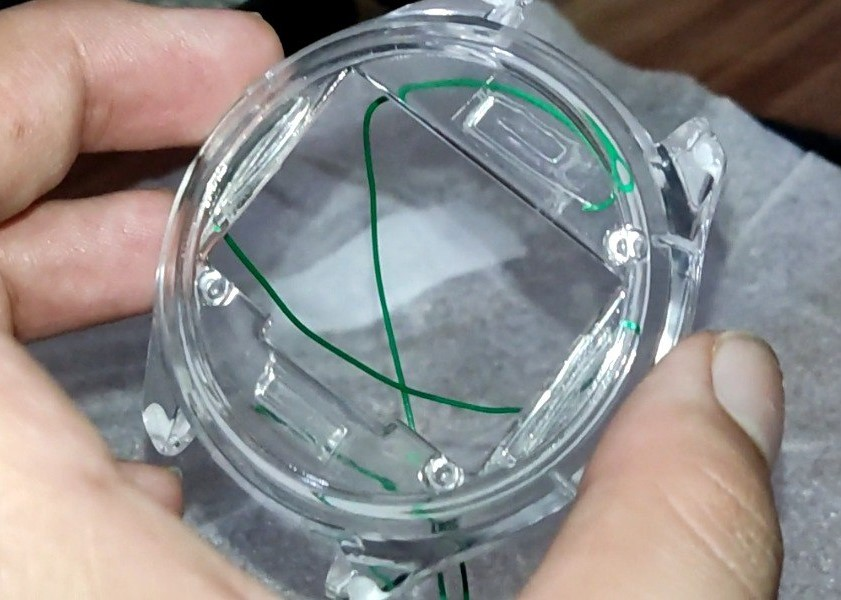
\includegraphics[width=\linewidth]{conn-touch2}
			\caption{چهار کلید نصب شده در چهار سمت بدنه}
			%\label{fig:oled_real}
		\end{subfigure}
		\caption{تصاویر اتصال کلیدهای لمسی به بدنه}
		\label{fig:conn-touch}
	\end{figure}

\subsection{صفحه نمایش}
همانطور که بالاتر بحث شد، صفحه نمایش با قرار گیری در سه استوانه‌ی موجود در بدنه سر جای خود محکم می‌شود. شکل \ref{fig:conn-oled} گویای این موضوع است.

	\begin{figure}[h]
		\centering
		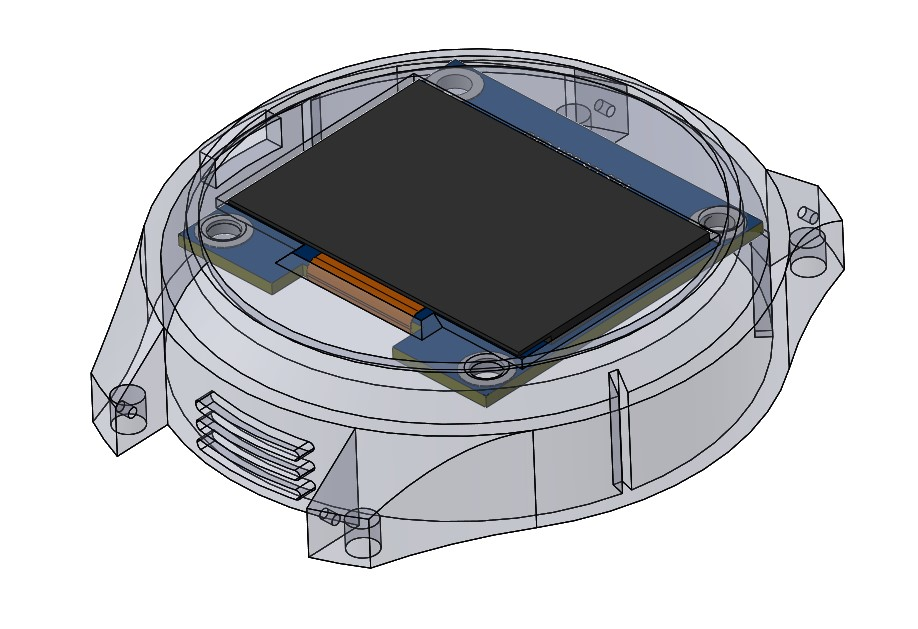
\includegraphics[width=0.5\linewidth]{conn_oled}
		\caption{تصویر اتصال صفحه نمایش به بدنه}
		\label{fig:conn-oled}
	\end{figure}

\subsection{\pcbf}
همانطور که بالاتر بحث شد، \pcbf با قرار گیری روی سه زائده‌ی موجود در بدنه سر جای خود محکم می‌شود. شکل \ref{fig:conn-pcb} گویای این موضوع است.

علت آن که برای اتصال صفحه نمایش یک استوانه از چهار استوانه حذف شده است آن است که استوانه‌ی حذف شده دقیقا بالای موتور ایجاد لرزش قرار داشت و در صورت وجود، به آن گیر می‌کرد و مانع جا گیری صحیح \pcbf می‌شد.

برای جلوگیری از اتصال ناخواسته و اتصال کوتاه بین صفحه نمایش و \pcbf، یک ورق نازک فوم بین این دو قرار گرفته است.

	\begin{figure}[h]
		\centering
		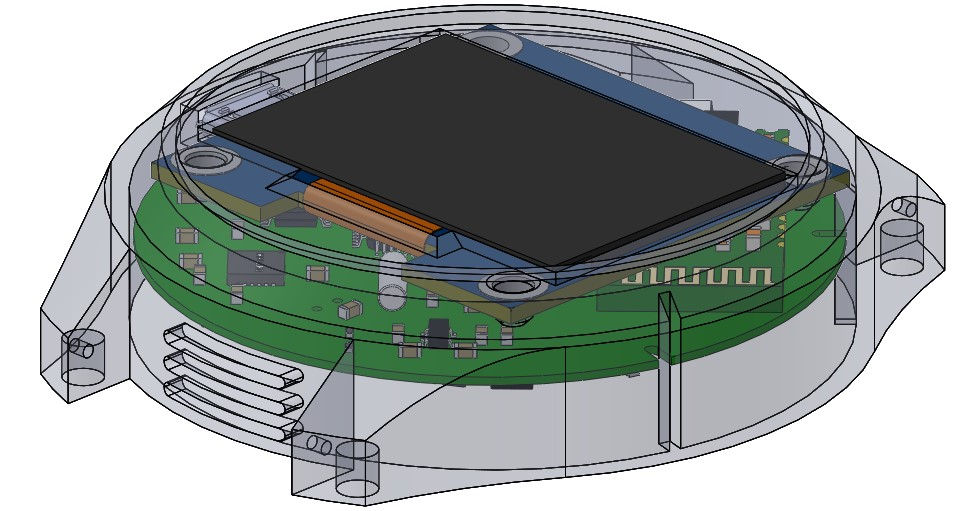
\includegraphics[width=0.5\linewidth]{conn_pcb}
		\caption{تصویر اتصال \pcbf به بدنه}
		\label{fig:conn-pcb}
	\end{figure}

\subsection{باتری}
باتری ساعت به کمک نوار چسب به \pcbf می‌چسبد و در جای خود محکم می‌شود. سیم‌های آن به محل خود لحیم شده و اتصال برقرار می‌شود. شکل \ref{fig:conn-battery} این اتصال را نشان می‌دهد.

	\begin{figure}[h]
		\centering
		\begin{subfigure}{0.5\textwidth}
			\centering
			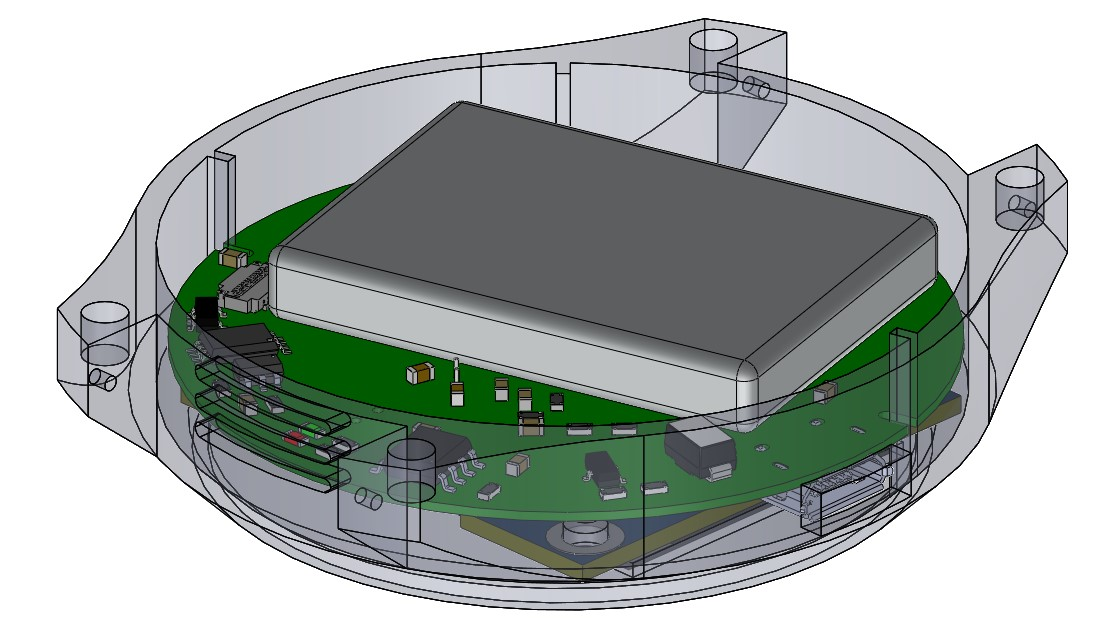
\includegraphics[width=\linewidth]{conn_battery}
			\caption{تصویر اتصال باتری در سالیدورکز}
			%\label{fig:oled_image}
		\end{subfigure} 
		\begin{subfigure}{0.4\textwidth}
			\centering
			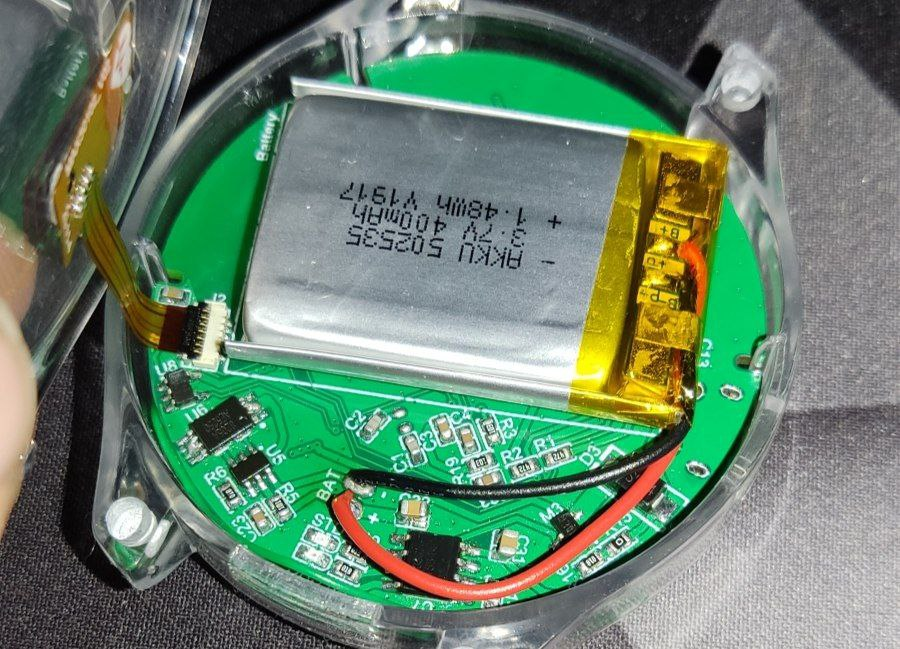
\includegraphics[width=\linewidth]{conn_battery2}
			\caption{تصویر واقعی باتری و اتصال آن}
			%\label{fig:oled_real}
		\end{subfigure}
		\caption{تصاویر اتصال باتری}
		\label{fig:conn-battery}
	\end{figure}

\subsection{حسگر \lr{PPG}}
این حسگر روی دریچه‌ی پشتی نصب می‌شود. همانطور که در شکل \ref{fig:conn-ppg} مشاهده می‌شود این حسگر به دریچه متصل است و سمت دیگر آن در جای مخصوص خود به \pcbf اتصال دارد. سوراخ مستطیل شکل روی دریچه و ضخامت مناسب آن باعث می‌شود سطح حسگر مماس سطح بیرونی دریچه باشد. اینگونه نه بیرون زدگی دارد تا آسیب ببیند و نه سطح آن از پوست فاصله می‌گیرد.

\begin{figure}[h]
	\centering
	\begin{subfigure}{0.405\textwidth}
		\centering
		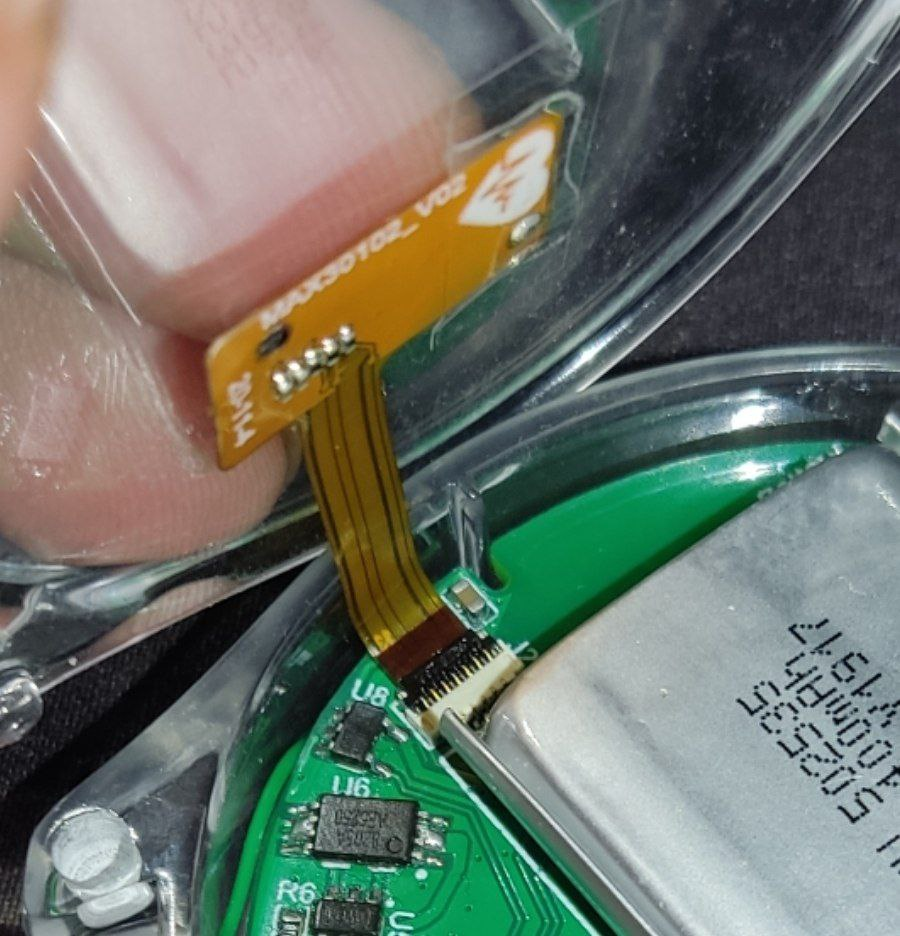
\includegraphics[width=\linewidth]{conn_ppg}
		\caption{نمای درونی}
		%\label{fig:oled_image}
	\end{subfigure} 
	\begin{subfigure}{0.4\textwidth}
		\centering
		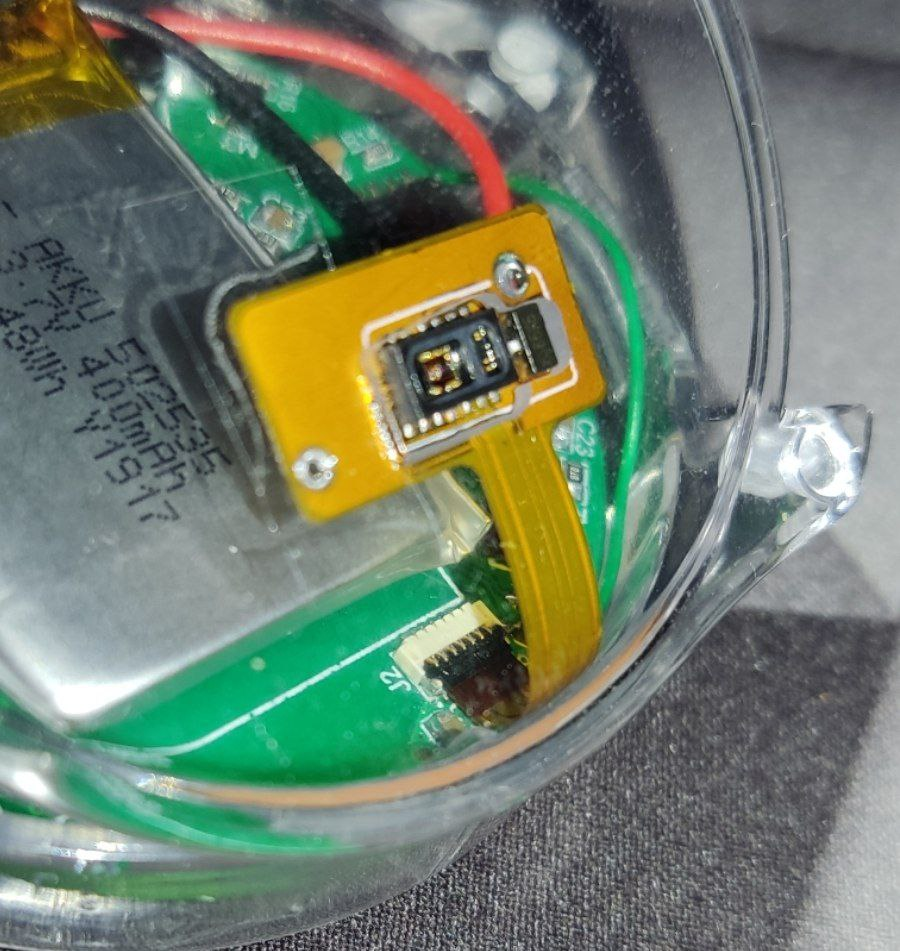
\includegraphics[width=\linewidth]{conn_ppg2}
		\caption{نمای بیرونی}
		%\label{fig:oled_real}
	\end{subfigure}
	\caption{تصاویر اتصال حسگر \lr{PPG}}
	\label{fig:conn-ppg}
\end{figure}

\subsection{دریچه‌ی پشتی}
دریچه‌ی پشتی مطابق با شکل \ref{fig:conn-back} به کمک چهار استوانه‌ی موجود روی آن به بدنه‌ی اصلی متصل می‌شود.

	\begin{figure}[h]
		\centering
		\begin{subfigure}{0.5\textwidth}
			\centering
			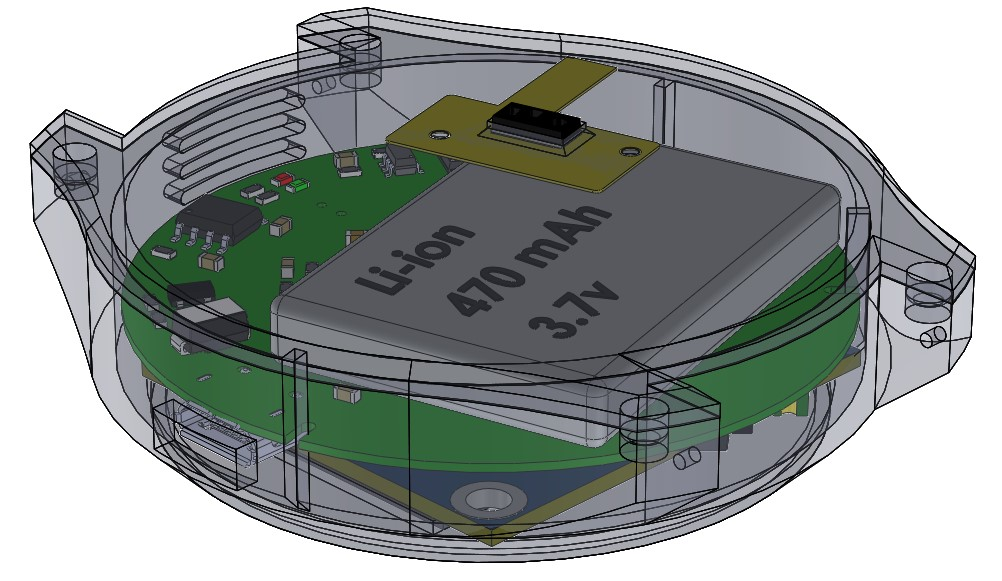
\includegraphics[width=\linewidth]{conn_back}
			\caption{تصویر اتصال دریچه در سالیدورکز}
			%\label{fig:oled_image}
		\end{subfigure} 
		\begin{subfigure}{0.4\textwidth}
			\centering
			\includegraphics[width=\linewidth]{conn_back2}
			\caption{تصویر واقعی دریچه و اتصال آن}
			%\label{fig:oled_real}
		\end{subfigure}
		\caption{تصاویر اتصال دریچه‌ی پشتی}
		\label{fig:conn-back}
	\end{figure}

در نهایت بدنه و مکانیک ساعت تکمیل شد و ظاهر نهایی ساعت به شکل \ref{fig:body-final} در آمد.

	\begin{figure}[h]
		\centering
		\begin{subfigure}{0.4\textwidth}
			\centering
			\includegraphics[width=\linewidth]{body_full}
			\caption{نمای رو}
			%\label{fig:oled_image}
		\end{subfigure} 
		\begin{subfigure}{0.4\textwidth}
			\centering
			\includegraphics[width=\linewidth]{body_full2}
			\caption{نمای زیر}
			%\label{fig:oled_real}
		\end{subfigure}
		\caption{تصاویر بدنه‌ی کامل}
		\label{fig:body-final}
	\end{figure}
%\chapter{نرم‌افزار}

در این فصل به جزئیات نرم‌افزار پرداخته می‌شود. منظور از نرم‌افزار، کدهایی است که نوشته شده‌اند تا توسط پردازنده‌ی روی ساعت اجرا شوند. در اصطلاح فنی به این بخش سفت‌افزار\footnote{\lr{Firmware}} نیز می‌گویند.

بین سفت‌افزار (برنامه‌ای که روی ریزپردازنده‌ها اجرا می‌شود) و نرم‌افزارهایی که برای سیستم‌های سطح بالا مانند رایانه نوشته می‌شود، تفاوت‌های بسیاری وجود دارد. برای مثال به چند نمونه از این تفاوت‌ها اشاره می‌کنیم:

\begin{enumerate}
	\item عدم وجود سیستم عامل: \\
	برنامه‌هایی که به زبان‌های مختلفی مانند \lr{C} یا \lr{Python} برای رایانه‌ها نوشته می‌شوند، توسط سیستم عامل اجرا می‌شوند. سیستم عامل وظیفه دارد تا برنامه‌های متنوعی که روی سیستم وجود دارد را زمان‌بندی کند، با مدیریت صحیح حافظه آن‌ها را اجرا کند و ارتباط با سخت‌افزار را نیز برعهده بگیرد. اما در حالتی که برای یک ریزپردازنده برنامه می‌نویسیم، دیگر سیستم عاملی وجود ندارد. بلکه تمام برنامه خط به خط و مستقیماً توسط ریزپردازنده اجرا می‌شود.
	
	\item ارتباط مستقیم با سخت‌افزار: \\
	در سیستم‌های سطح بالا که به سیستم عامل مجهزند، ارتباط با سخت‌افزار نیز برعهده‌ی سیستم عامل است. در صورتی که نیاز باشد با دستگاه‌های ورودی/خروجی ارتباطی برقرار شود، از طریق توابع سیستمی موجود در سیستم عامل این ارتباط ایجاد می‌شود. اما هنگام نوشتن برنامه برای ریزپردازنده، باید لایه‌ی ارتباط با سخت‌افزار را نیز نوشت. زیرا سیستم عاملی وجود ندارد و تک تک ارتباطات سخت‌افزاری باید توسط برنامه نویس راه‌اندازی شود.
	
	\item مدیریت حافظه: \\
	هنگامی که در برنامه‌ای به زیان \lr{C} می‌خواهیم از قسمتی از حافظه استفاده کنیم، باید با دستور \lr{malloc} و نظایر آن، به سیستم عامل درخواست دهیم تا آدرس مناسبی را به برنامه‌ی ما اختصاص دهد. همچنین در صورتی که بخواهیم در آدرسی که به برنامه‌ی ما تعلق ندارد مقداری را بنویسیم یا از آن بخوانیم، سیستم عامل مانع می‌شود و با خطای عدم دسترسی مواجه می‌شویم. اما در موردی که با ریزپردازنده‌ها سر و کار داشته باشیم دیگر نیازی به درخواست و اختصاص حافظه نیست. چرا که سیستم عاملی وجود ندارد و تمام حافظه در اختیار برنامه‌ی ما است. در این حالت مدیریت حافظه امری بسیار حساس است. زیرا چیزی وجود ندارد تا مانع دسترسی‌های اشتباه شود و ممکن است با خطا در مدیریت حافظه، عملکرد برنامه دچار اختلالات جدی شود.
	
	\item محدودیت منابع: \\
	پردازنده‌ی رایانه‌ها معمولاً پردازنده‌های قوی‌ای هستند و سرعت بالایی دارند. همچنین حافظه‌های موجود نیز بسیار زیاد هستند. حال آنکه در پردازنده‌ها این منابع بسیار بسیار محدود هستند. همانطور که در ضمیمه‌ی ؟ قابل مشاهده است، مقدار حافظه‌ی فلش ریزپردازنده‌ی ما فقط 64 کیلوبایت است. به این معنی که حجم برنامه بعد از کامپایل نباید از این مقدار تجاوز کند. این محدودیت هرگز در نرم‌افزارهای رایج وجود ندارد. این اتفاق باعث می‌شود تا برنامه نویسی برای ریزپردازنده‌ها دشوارتر شود و نیاز به دانش بیشتری داشته باشد تا بتوان با بهینه‌سازی‌های مختلف و الگوریتم‌های بهتر، حجم برنامه را کاهش داد. در ادامه یکی از این بهینه‌سازی‌ها در رابطه با پیاده‌سازی فیلتر کالمن توضیح داده خواهد شد.
\end{enumerate}

\section{تنظیمات سخت‌افزاری}
همانطور که بالاتر اشاره شد، ارتباط با سخت‌افزار باید توسط برنامه رسیدگی شود. برای این هدف از نرم‌افزار \lr{CubeMX} استفاده شد. شکل \ref{fig:cube-main} نحوه‌ی اختصاص پایه‌ها را نشان می‌دهد. هر کدام از بخش‌ها به تفصیل در ادامه بررسی می‌شود.

	\begin{figure}[h]
		\centering
		\includegraphics[width=0.9\linewidth]{cube}
		\caption{نحوه‌ی تخصیص پایه‌های مختلف ریزپردازنده در نرم‌افزار \lr{CubeMX}}
		\label{fig:cube-main}
	\end{figure}

\subsection{کلاک}
تنظیمات کلاک به صورت شکل \ref{fig:cube-rcc} است. نوسان‌ساز اصلی روی 8 مگاهرتز داخلی تنظیم شده است و برای ایجاد کلاک بخش ساعت و تاریخ، از یک کریستال خارجی با فرکانس 768.32 کلیوهرتز استفاده شده است. کلاک بخش‌های مختلف نیز در همین تصویر قابل مشاهده است.

	\begin{figure}[h]
		\centering
		\includegraphics[width=0.9\linewidth]{cube_rcc}
		\caption{تنظیمات کلاک}
		\label{fig:cube-rcc}
	\end{figure}

\subsection{برنامه‌ریزی و اشکال‌زدایی}
برای بحث برنامه‌ریزی\footnote{انتقال برنامه‌ی نوشته شده به ریزپردازنده یا به اصطلاح \lr{Programming}} و اشکال‌زدایی\footnote{\lr{Debugging}} از پروتکل \lr{Serial Wire} استفاده شده است که در شکل \ref{fig:cube-sys} تنظیم آن دیده می‌شود.

	\begin{figure}[h]
		\centering
		\includegraphics[width=0.4\linewidth]{cube_sys}
		\caption{تنظیمات \lr{Debugging}}
		\label{fig:cube-sys}
	\end{figure}

\subsection{\lr{GPIO}}\label{sec:gpio}
\lr{GPIO}ها پایه‌هایی هستند که به عنوان ورودی/خروجی دیجیتال مورد استفاده قرار می‌گیرند. در این پروژه از \lr{GPIO}های متعددی استفاده شده است که در شکل \ref{fig:cube-gpio} فهرست آن‌ها قابل مشاهده است. در ادامه هر مورد توضیح داده می‌‌شود.

	\begin{figure}[h]
		\centering
		\includegraphics[width=\linewidth]{cube_gpio}
		\caption{تنظیمات \lr{GPIO}}
		\label{fig:cube-gpio}
	\end{figure}

\subsubsection{وقفه‌های خارجی}
وقفه‌های خارجی\footnote{\lr{External intrrupts}}
پایه‌هایی هستند که در صورت وقوع رویداد خاصی، کار عادی پردازنده را متوقف می‌کنند و یک تابع به خصوص را به اجرا در می‌آورند. بعد از اجرای روتین وقفه، پردازنده به کار قبلی خود ادامه می‌دهد.

رویدادهای مورد استفاده در این پروژه دو مورد است: 1- لبه‌ی پایین رونده\footnote{\lr{Falling Edge}}
2- لبه‌ی بالا رونده\footnote{\lr{Rising Edge}}
همانطور که در شکل \ref{fig:cube-gpio} مشهود است، پایه‌های 3، 4، 5 و 8 از پورت \lr{B} و پایه‌ی 15 از پورت \lr{A} برای لبه‌ی بالارونده تنظیم شده‌اند. پایه‌ی 9 از پورت \lr{B} نیز به لبه‌ی پایین رونده حساس است.

اینکه کدام پایه توسط کدام بخش تحریک می‌شود در ستون \lr{User label} شکل \ref{fig:cube-gpio} دیده می‌شود. برچسب‌های \lr{KEY} مربوطه به کلیدهای لمسی روی بدنه هستند. در صورت لمس شدن هر کلید، تابع مخصوص آن اجرا می‌شود. برچسب \lr{MPU} مربوط به حسگر حرکتی است. این پایه وقتی فعال می‌شود که داده‌های جدید حسگر آماده شده باشد. برچسب \lr{MAX} نیز به همین شکل عمل می‌کند. هرگاه داده‌ی حسگر \lr{PPG} آماده‌ی قرائت باشد، این وقفه فعال می‌شود.

\subsubsection{خروجی دیجیتال}
پایه‌ی 13 از پورت \lr{C} به صورت خروجی دیجیتال تعریف شده است. این خروجی به پایه‌ی فعالساز سوییچ ماسفتی متصل است که حسگر \lr{PPG} را روشن می‌کند (شکل \ref{fig:sch-ppg}). برای روشن یا خاموش کردن این حسگر، کافی است این پایه را صفر یا یک کرد.

\subsection{\lr{RTC}}
واحد
\lr{RTC}\footnote{\lr{Real-time Clock}}
برای نگهداری و کار با ساعت و تاریخ است. تنظیمات این بخش در شکل \ref{fig:cube-rtc} دیده می‌شود. در این بخش می‌توان یک آلارم هم فعال کرد که در ساعت و روز مشخصی یک وقفه را فعال کند. در اینجا آلارم هم فعال شده است.

	\begin{figure}[h]
		\centering
		\includegraphics[width=0.45\linewidth]{cube_rtc}
		\caption{تنظیمات \lr{RTC}}
		\label{fig:cube-rtc}
	\end{figure}

\subsection{تایمرها}
این ریزپردازنده هفت تایمر دارد که در این پروژه هر هفت تایمر استفاده شده‌اند. در ادامه کاربرد و تنظیمات هر تایمر شرح داده می‌شود.

\subsubsection{\lr{TIM1}}
تایمر شماره‌ی یک مطابق با تنظیمات شکل \ref{fig:cube-tim1} راه‌اندازی شده است تا بتواند \lr{PWM} موردنیاز برای کنترل دور موتور ایجاد لرزش را تولید کند. البته مقدار رجیستر
\lr{ARR}\footnote{\lr{Auto-Reload Register} رجیستری است که برای تنظیم فرکانس اصلی تایمر استفاده می‌شود}
در برنامه به صورت پویا تغییر می‌کند.

\subsubsection{\lr{TIM3}}
تایمر شماره‌ی یک مطابق با تنظیمات شکل \ref{fig:cube-tim3} راه‌اندازی شده است تا بتواند \lr{PWM} موردنیاز برای تنظیم فرکانس صدای بازر را تولید کند. البته مقدار رجیستر
\lr{ARR}
در برنامه به صورت پویا تغییر می‌کند.

	\begin{figure}[h]
		\centering
		\begin{subfigure}{0.4\textwidth}
			\centering
			\includegraphics[width=\linewidth]{cube_tim1}
			\caption{تنظیمات تایمر یک}
			\label{fig:cube-tim1}
		\end{subfigure}
		\begin{subfigure}{0.44\textwidth}
			\centering
			\includegraphics[width=\linewidth]{cube_tim3}
			\caption{تنظیمات تایمر سه}
			\label{fig:cube-tim3}
		\end{subfigure}
		\caption{تنظیمات دو تایمر}
		%\label{fig:body-pcb}
	\end{figure}

\subsubsection{\lr{TIM6}}
تایمر شماره‌ی شش مطابق شکل \ref{fig:cube-tim6} تنظیم شده است تا هر یک میلی ثانیه یک وقفه را فعال کند. این وقفه توابع مربوط به فیلتر کالمن را اجرا می‌کند. در واقع می‌توان گفت دوره تناوب نمونه‌گیری و پردازش سیستم کالمن یک میلی ثانیه است.

	\begin{figure}[h]
		\centering
		\includegraphics[width=0.43\linewidth]{cube_tim6}
		\caption{تنظیمات تایمر شش}
		\label{fig:cube-tim6}
	\end{figure}

\subsubsection{\lr{TIM14}}
تایمر شماره‌ی چهارده مطابق شکل \ref{fig:cube-tim14} تنظیم شده است تا هر 250 میلی ثانیه یک وقفه را فعال کند. این وقفه مربوط به توابع سیستمی است. در این توابع مواردی از قبیل تازه‌سازی صفحه نمایش و تنظیم برخی متغیرها انجام می‌شود.


	\begin{figure}[h]
		\centering
		\includegraphics[width=0.35\linewidth]{cube_tim14}
		\caption{تنظیمات تایمر چهارده}
		\label{fig:cube-tim14}
	\end{figure}

\subsubsection{\lr{TIM15}}
تایمر شماره‌ی پانزده مطابق شکل \ref{fig:cube-tim15} تنظیم شده است تا هر 10 میلی ثانیه به واحد \lr{ADC} فرمانِ تبدیل دهد. به این معنی که واحد آنالوگ به دیجیتال فقط در صورتی یک نمونه‌برداری را شروع می‌کند که تایمر شماره 15 به آن فرمان دهد. اینگونه یک نمونه‌برداری دقیق زمانی ایجاد می‌شود.

	\begin{figure}[h]
		\centering
		\includegraphics[width=0.4\linewidth]{cube_tim15}
		\caption{تنظیمات تایمر پانزده}
		\label{fig:cube-tim15}
	\end{figure}

\subsubsection{\lr{TIM16}}
تایمر شماره‌ی شانزده مطابق شکل \ref{fig:cube-tim16} تنظیم شده است تا هر 4 ثانیه یک وقفه را فعال کند. این وقفه برای خاموش کردن صفحه نمایش است. هرگاه کاربر به مدت 4 ثانیه با ساعت تعامل نداشته باشد این وقفه صفحه را خاموش می‌کند.

	\begin{figure}[h]
		\centering
		\includegraphics[width=0.4\linewidth]{cube_tim16}
		\caption{تنظیمات تایمر شانزده}
		\label{fig:cube-tim16}
	\end{figure}

\subsubsection{\lr{TIM17}}
تایمر شماره‌ی هفده مطابق شکل \ref{fig:cube-tim17} تنظیم شده است. این تایمر وقفه ندارد و به صورت یک زمان‌سنج به کار می‌رود. از این تایمر برای ساخت تابع تأخیر استفاده شده است. حداکثر تأخیر قابل تولید توسط این تایمر، دو به توان 16 یعنی 65536 میلی ‌ثانیه است. 

	\begin{figure}[h]
		\centering
		\includegraphics[width=0.4\linewidth]{cube_tim17}
		\caption{تنظیمات تایمر هفده}
		\label{fig:cube-tim17}
	\end{figure}

\subsection{\lr{ADC}}
مبدل آنالوگ به دیجیتال در این پردازنده 12 بیتی است. یعنی ولتاژ ورودی را از بازه‌ی 0 تا 3.3 ولت به بازه‌ی 0 تا 4095 نگاشت می‌کند. اینگونه می‌توان با یک ضرب و تقسیم ساده مقدار ولتاژ ورودی را خواند. شکل \ref{fig:cube-adc} تنظیمات این واحد را نشان می‌دهد. همانطور که گفته شد، این واحد به کمک تایمر 15 فعال می‌شود و با هر فرمان آن یک نمونه برمی‌دارد. برای ذخیره‌ی این نمونه‌ها، \lr{ADC} را با
\lr{DMA}\footnote{\lr{Direct Memory Access}}
کوپل می‌کنیم. اینگونه هربار که \lr{ADC} یک نمونه را تبدیل کرد، به طور مستقیم و بدون دخالت پردازنده آن را در یک آرایه ذخیره می‌کند. بعد از اینکه آرایه پر شد نیز با فعال کردن یک وقفه به ما خبر می‌دهد تا عملیات پردازشی روی آن انجام گیرد.

این ساختار که \lr{ADC} با تایمر فعال شود و با \lr{DMA} کار کند، حرفه‌ای ترین ساختار راه‌اندازی این واحد است. تنظیمات \lr{DMA} در شکل \ref{fig:cube-adc-dma} دیده می‌شود.

	\begin{figure}[h]
		\centering
		\begin{subfigure}{0.5\textwidth}
			\centering
			\includegraphics[width=\linewidth]{cube_adc}
			\caption{تنظیمات \lr{ADC}}
			\label{fig:cube-adc}
		\end{subfigure} \\
		\begin{subfigure}{0.54\textwidth}
			\centering
			\includegraphics[width=\linewidth]{cube_adc_dma}
			\caption{تنظیمات \lr{DMA}}
			\label{fig:cube-adc-dma}
		\end{subfigure}
		\caption{تنظیمات مبدل آنالوگ به دیجیتال}
	\end{figure}

\subsection{\lr{I2C}}
واحد \lr{I2C} مطابق شکل \ref{fig:cube-i2c} تنظیم شده است. این واحد یک واحد ارتباطی تحت پروتکل \lr{I2C} است.

	\begin{figure}[h]
		\centering
		\includegraphics[width=0.5\linewidth]{cube_i2c}
		\caption{تنظیمات \lr{I2C}}
		\label{fig:cube-i2c}
	\end{figure}

\subsection{\lr{USART}}
واحد \lr{USART1} و \lr{USART2} مطابق شکل \ref{fig:cube-usart} تنظیم شده و تنظیمات مشابهی دارند. با این تفاوت که \lr{USART2} به یک واحد \lr{DMA} نیز وصل است تا داده‌ی دریافتی بلوتوث را مستقیماً در حافظه ذخیره کند و در صورت تکمیل شدن پیام، وقفه‌ی مربوطه را فعال کند تا داده‌ی دریافتی پردازش شود.

	\begin{figure}[h]
		\centering
		\includegraphics[width=0.5\linewidth]{cube_usart}
		\caption{تنظیمات \lr{USART}}
		\label{fig:cube-usart}
	\end{figure}



\section{معماری}
برنامه‌ی نوشته شده در این پروژه مشابه برنامه‌های عادی ریزپردازنده‌ها نیست. در اکثر قریب به اتفاق پروژه‌ها، معماری به این صورت است که ابتدا چند تابع اجرا می‌شوند تا تنظیمات کلی را انجام دهند، سپس یک حلقه‌ی \lr{while(1)} وجود دارد تا روتین اصلی برنامه به صورت مداوم در آن اجرا شود. در این معماری وظیفه‌های\footnote{\lr{Tasks}}
مختلف به طور غیر همزمان اجرا شده و مشکلات زمان‌بندی دارند.

اما معماری این پروژه یک معماری رویداد محور\footnote{\lr{Event-based architecture}}
است. در این معماری حلقه‌ی \lr{while(1)} خالی است و تمام وظیفه‌ها در توابع وقفه رسیدگی می‌شوند.

در کنار این معماری رویداد محور، یک ماشین حالت محدود یا به اختصار
\lr{FSM}\footnote{\lr{Finite State Machine}}
نیز وجود دارد تا حالت‌های کاری مختلف را اجرا کند.

در ادامه بخش‌های مختلف این معماری شرح داده می‌شود.
\subsection{ماشین حالت} \label{sec:fsm}
ماشین حالت مفهومی است برای توصیف و تشریح عملکرد یک سیستم که حالت‌های کاری مختلفی دارد. این مفهوم نشان می‌دهد که چگونه هر حالت به حاتی دیگر تبدیل می‌شود و در هر حالت خروجی سیستم چیست.

	\begin{figure}[h]
		\centering
		\includegraphics[width=0.5\linewidth]{states}
		\caption{حالت‌های ماشین حالت}
		\label{fig:states}
	\end{figure}

در این پروژه ماشین حالت را تعمیم داده‌ام. به این صورت که انتقال بین حالت‌ها همچنان به کمک یک سیگنال کلاک صورت می‌گیرد، اما دیگر هر حالت خروجی ثابتی ندارد، بلکه مجموعه‌ای ای توابع در هر حالت دائماً اجرا می‌شوند. شکل \ref{fig:states} حالت‌ها و نام آن‌ها را نشان می‌دهد.

\subsubsection{حالت در انتظار تایید}
\begin{itemize}
	\item روتین اصلی:
		\begin{enumerate}
			\item نمایش صفحه‌ی درخواست تایید مطابق شکل \ref{fig:state-ack}
			\item متوقف کردن تایمر خاموش کردن صفحه نمایش
		\end{enumerate}
	\item کلید بالا فشرده شود:
		\begin{enumerate}
			\item یک کردن متغیر \lr{ack} در ساختار سیستم
			\item فراخوانی تابع سیستمی ارسال تاییدیه
		\end{enumerate}
	\item کلید پایین فشرده شود:
		\begin{enumerate}
			\item صفر کردن متغیر \lr{ack} در ساختار سیستم
			\item فراخوانی تابع سیستمی ارسال عدم تایید
			\item تنظیم حالت روی خانه
			\item فعال کردن صفحه نمایش
		\end{enumerate}
\end{itemize}
	\begin{figure}[h]
		\centering
		\includegraphics[width=0.3\linewidth]{state_ack} %%%%%%%%%%%%%%%%%%%%%%%%%%%%%%%%%%%%%%%%
		\caption{صفحه‌ی در انتظار تایید}
		\label{fig:state-ack}
	\end{figure}

\subsubsection{حالت خوش‌آمد گویی}
\begin{itemize}
	\item روتین اصلی:
	\begin{enumerate}
		\item نمایش صفحه‌ی خوش‌آمد گویی به مدت 4 ثانیه \ref{fig:state-hello}
		\item تنظیم حالت به عنوان خانه
		\item فعال کردن تایمر خاموش کردن صفحه
	\end{enumerate}
\end{itemize}
	\begin{figure}[h]
		\centering
		\includegraphics[width=0.3\linewidth]{state_ack} %%%%%%%%%%%%%%%%%%%%%%%%%%%%%%%%%%%%%%%%%%%%
		\caption{صفحه‌ی خوش‌آمد گویی}
		\label{fig:state-hello}
	\end{figure}

\subsubsection{حالت خانه}
\begin{itemize}
	\item روتین اصلی:
	\begin{enumerate}
		\item قرائت ساعت و تاریخ
		\item قرائت میزان شارژ باتری
		\item قرائت وضعیت اتصال به گوشی
		\item نمایش صفحه‌ی اصلی مطابق شکل \ref{fig:state-home}
	\end{enumerate}
	\item کلید بالا فشرده شود:
	\begin{enumerate}
		\item تنظیم حالت روی درباره‌ی ما
	\end{enumerate}
	\item کلید پایین فشرده شود:
	\begin{enumerate}
		\item متوقف کردن تایمر فیلتر کالمن
		\item متوقف کردن تایمر \lr{ADC}
		\item روشن کردن حسگر \lr{PPG} و تنظیم آن
		\item تنظیم حالت روی حسگر سلامت
	\end{enumerate}
\end{itemize}
	\begin{figure}[h]
		\centering
		\includegraphics[width=0.3\linewidth]{state_ack} %%%%%%%%%%%%%%%%%%%%%%%%%%%%%%%%%%%%%%%%
		\caption{صفحه‌ی اصلی}
		\label{fig:state-home}
	\end{figure}

\subsubsection{حالت حسگر سلامت}
\begin{itemize}
	\item روتین اصلی:
	\begin{enumerate}
		\item نمایش صفحه‌ی حسگر سلامت مطابق شکل \ref{fig:state-bloody}
		\item متوقف کردن تایمر خاموش کردن صفحه نمایش
	\end{enumerate}
	\item کلید بالا فشرده شود:
	\begin{enumerate}
		\item خاموش کردن حسگر سلامت
		\item روشن کردن تایمر فیلتر کالمن
		\item روشن کردن تایمر \lr{ADC}
		\item روشن کردن تایمر خاموش شدن صفحه نمایش
		\item تنظیم حالت روی خانه
	\end{enumerate}
	\item کلید پایین فشرده شود:
	\begin{enumerate}
		\item خاموش کردن حسگر سلامت
		\item روشن کردن تایمر فیلتر کالمن
		\item روشن کردن تایمر \lr{ADC}
		\item تنظیم حالت روی حسگر حرکتی
	\end{enumerate}
\end{itemize}
	\begin{figure}[h]
		\centering
		\includegraphics[width=0.3\linewidth]{state_ack} %%%%%%%%%%%%%%%%%%%%%%%%%%%%%%%%%%%%%%%%
		\caption{صفحه‌ی حسگر سلامت}
		\label{fig:state-bloody}
	\end{figure}
\subsubsection{حالت حسگر حرکتی}
\begin{itemize}
	\item روتین اصلی:
	\begin{enumerate}
		\item نمایش صفحه‌ی حسگر حرکتی مطابق شکل \ref{fig:state-pedomedo}
		\item متوقف کردن تایمر خاموش کردن صفحه نمایش
	\end{enumerate}
	\item کلید بالا فشرده شود:
	\begin{enumerate}
		\item متوقف کردن تایمر فیلتر کالمن
		\item متوقف کردن تایمر \lr{ADC}
		\item روشن کردن حسگر \lr{PPG} و تنظیم آن
		\item تنظیم حالت روی حسگر سلامت
	\end{enumerate}
	\item کلید پایین فشرده شود:
	\begin{enumerate}
		\item تنظیم حالت روی درباره‌ی ما
	\end{enumerate}
\end{itemize}
	\begin{figure}[h]
		\centering
		\includegraphics[width=0.3\linewidth]{state_ack} %%%%%%%%%%%%%%%%%%%%%%%%%%%%%%%%%%%%%%%%
		\caption{صفحه‌ی حسگر حرکتی}
		\label{fig:state-pedomedo}
	\end{figure}

\subsubsection{حالت درباره‌ی ما}
\begin{itemize}
	\item روتین اصلی:
	\begin{enumerate}
		\item نمایش صفحه‌ی درباره‌ی ما مطابق شکل \ref{fig:state-about}
		\item متوقف کردن تایمر خاموش کردن صفحه نمایش
	\end{enumerate}
	\item کلید بالا فشرده شود:
	\begin{enumerate}
		\item تنظیم حالت روی حسگر حرکتی
	\end{enumerate}
	\item کلید پایین فشرده شود:
	\begin{enumerate}
		\item روشن کردن تایمر خاموش شدن صفحه نمایش
		\item تنظیم حالت روی خانه
	\end{enumerate}
\end{itemize}
	\begin{figure}[h]
		\centering
		\includegraphics[width=0.3\linewidth]{state_ack} %%%%%%%%%%%%%%%%%%%%%%%%%%%%%%%%%%%%%%%%
		\caption{صفحه‌ی درباره‌ی ما}
		\label{fig:state-about}
	\end{figure}
\subsubsection{حالت آلارم}
\begin{itemize}
	\item روتین اصلی:
	\begin{enumerate}
		\item نمایش صفحه‌ی آلارم مطابق شکل \ref{fig:state-ringing}
		\item متوقف کردن تایمر خاموش کردن صفحه نمایش
	\end{enumerate}
	\item هر کلیدی که فشرد شود:
	\begin{enumerate}
		\item پایین آوردن پرچم آلارم
		\item روشن کردن تایمر فیلتر کالمن
		\item روشن کردن تایمر خاموش شدن صفحه نمایش
		\item تنظیم حالت روی خانه
	\end{enumerate}
\end{itemize}
	\begin{figure}[h]
		\centering
		\includegraphics[width=0.3\linewidth]{state_ack} %%%%%%%%%%%%%%%%%%%%%%%%%%%%%%%%%%%%%%%%
		\caption{صفحه‌ی آلارم}
		\label{fig:state-ringing}
	\end{figure}


\subsection{وقفه‌ها}
منابع وقفه در این پروژه 5 چیز است:
\begin{enumerate}
	\item وقفه‌ی خارجی\footnote{\lr{EXTI (External Interupt)}}:
	همانطور که در بخش \ref{sec:gpio} بحث شد، 5 پایه از پایه‌های \lr{GPIO} برای فعالسازی وقفه‌ی خارجی هستند:
	\begin{enumerate}
		\item کلیدهای لمسی:
		بعد از فعال شدن وقفه، با توجه به اینکه سیستم در چه حالتی از حالت‌های هفتگانه قرار دارد، توابع مشخصی اجرا می‌شوند. شرح کامل این اقدامات در بخش \ref{sec:fsm} داده شده است. شکل \ref{fig:exti} یک نمونه از این کدها را نشان می‌دهد.
		\begin{figure}[h]
			\centering
			\includegraphics[width=0.4\linewidth]{exti}
			\caption{نمونه کدی از بخش وقفه‌ی خارحی}
			\label{fig:exti}
		\end{figure}
	
		\item وقفه‌ی حسگر \lr{PPG}: هنگامی که حسگر داده‌ی جدیدی داشته باشد، با فعال کردن یک پایه، وقفه‌ای را فعال می‌کند. در روتین این وقفه داده‌های حسگر قرائت می‌شود و به ترتیب در یک آرایه ذخیره می‌شوند. هنگامی که این آرایه پر شود، توسط بلوتوث به گوشی ارسال می‌گردد. شکل \ref{fig:exti-ppg} بخش مربوط به ذخیره در آرایه و ارسال آن را نشان می‌دهد.
		\begin{figure}[h]
			\centering
			\includegraphics[width=0.7\linewidth]{exti_ppg}
			\caption{نمونه کدی از بخش ذخیره‌ی داده‌ی حسگر سلامت}
			\label{fig:exti-ppg}
		\end{figure}
		
	\end{enumerate}
	\item وقفه‌ی تایمر:
	همانطور که گفته شد سه تایمر از هفت تایمر برای فعالسازی وقفه به کار رفته‌اند:
	\begin{enumerate}
		\item تایمر فیلتر کالمن:
		این تایمر هر یک میلی ثانیه وقفه را فعال می‌کند. در روتین وقفه ابتدا اطلاعات حسگر حرکتی خوانده می‌شود. سپس این اطلاعات برای فیلتر شدن به توابع کالمن داده می‌شود. شرج این توابع در بخش‌هایی بعدی آورده شده است. سپس اطلاعات فیلتر شده وارد مرحله‌ی پردازش می‌شوند. این پردازش‌ها شامل تشخیص سرعت زاویه‌ای دست حول آرنج و تشخیص گام است. کد این بخش در شکل \ref{fig:kalman-code} قابل مشاهده است.
		\begin{figure}[h]
			\centering
			\includegraphics[width=0.45\linewidth]{kalman_code}
			\caption{نمونه کدی از بخش وقفه‌ی کالمن}
			\label{fig:kalman-code}
		\end{figure}
		
		\item تایمر صفحه نمایش:
		هرگاه وقفه‌ی این تایمر فعال شود به این معنی است که چهار ثانیه از آخرین تعامل کاربر با ساعت گذشته است و باید صفحه نمایش خاموش شود. شکل \ref{fig:screen-timer} کد این قسمت را نشان می‌دهد.
		\begin{figure}[h]
			\centering
			\includegraphics[width=0.4\linewidth]{screen_timer}
			\caption{کد روتین وقفه‌ی تایمر صفحه نمایش}
			\label{fig:screen-timer}
		\end{figure}
		
		\item تایمر اصلی سیستم:
این تایمر هر 250 میلی ثانیه سرریز می‌شود. در نتیجه هر 250 میلی ثانیه روتین وقفه اجرا می‌شود. در روتین وقفه‌ی این تایمر ابتدا بررسی می‌شود که آیا صفحه نمایش باید روشن شود یا خیر. اگر نیاز به روشن شدن بود، با توجه به حالت سیستم و ماشین حالتی که در بخش \ref{sec:fsm} توضیح داده شد، روتین حالت مربوطه را اجرا می‌کند.
	\end{enumerate}
	\item وقفه‌ی آلارم:
	هنگامی که ساعت و روز بر ساعت و روز آلارم منطبق شود، این وقفه فعال می‌گردد. در روتین این وقفه پرچم آلارم یک می‌شود، تایمر کالمن خاموش می‌شود، صفحه نمایش روشن می‌شود و حالت سیستم به آلارم تغییر می‌کند.
	\item وقفه‌ی \lr{DMA} مربوطه به \lr{ADC}:
	تنظیمات \lr{DMA} مربوط به \lr{ADC} به گونه‌ای است که \lr{ADC} هر 10 میلی ثانیه یک نمونه می‌گیرد و آن را در آرایه‌ای ذخیره می‌کند. هرگاه این آرایه که طول آن 128 است پر شود، این وقفه فعال می‌شود. در روتین وقفه می‌خواهیم میانگین این 128 نمونه را به عنوان عدد نهایی گزارش کنیم. میانگین ساده‌ترین راه جلوگیری از ورود نویز به سیستم است.
	
	پس مطابق شکل \ref{fig:adc-dma} ابتدا مجموع این 128 داده را حساب می‌کنیم. سپس باید این حاصل را بر تعداد نمونه‌ها تقسیم کنیم. فلسفه‌ی انتخاب عدد 128 برای تعداد نمونه‌ها اینجا مشخص می‌شود. می‌دانیم تقسیمات اعشاری به دلیل پیچیدگی‌های محاسباتی، مقداری زیادی از حافظه را اشغال می‌کنند و سرعت کمتری دارند. پس بهتر است تا جای ممکن از آن‌ها دوری کنیم.
	
	از طرفی می‌دانیم که اگر مقسوم‌علیه توان دو باشد، می‌توان عملیات تقسیم را با شیفت مقسوم انجام داد. در اینجا جای اینکه مجموع را بر 128 تقسیم کنیم، کافی است آن را 7 بیت به سمت راست شیفت دهیم تا تقسیم انجام شود. اینگونه هم سرعت بسیار بالایی دارد هم حافظه را بیهوده اشغال نمی‌کند.
	\begin{figure}[h]
		\centering
		\includegraphics[width=0.4\linewidth]{adc_dma}
		\caption{کد روتین وقفه‌ی \lr{DMA} مربوطه به \lr{ADC}}
		\label{fig:adc-dma}
	\end{figure}
	\item وقفه‌ی \lr{DMA} مربوطه به \lr{UASRT}:
	لرزاایذتسنیرذاسرذنتمذرنتسرد ترذنتسرذنت ذرتذر متبذر مشب
\end{enumerate}
\subsection{لایه‌های نرم‌افزاری}

\section{ارتباطات}

\section{پردازش داده‌های حسگر حرکتی}
%\chapter{نرم‌افزار}

با این‌که چالش‌های متعددی در مسیر انجام این پروژه خودنمایی کردند، در این فصل صرفا به برخی از چالش‌های مهم‌تر خواهیم پرداخت که می‌توان آن‌ها را در سه دسته‌ی فرآیندی، معماری و محدودیت‌های چارچوبی دسته‌بندی کرد.

\section{؟}

%\subsection{ترکیب فرآیندهای ظاهر و باطن سامانه}

یکی از مهم‌ترین چالش‌های فرآیندی که در روال توسعه اسکرام در این پروژه مشخص شد، لزوم جداسازی \lr{Backlog}های ظاهر\footnote{\lr{Front-end}} و باطن\footnote{\lr{Back-end}} سامانه از یکدیگر بود. با توجه به اینکه در این پروژه از سامانه جیرا برای مدیریت فرآیند توسعه استفاده می‌شود، در ابتدا برای هر استوری کاربر، دو زیرمجموعه فرانت-اند و بک-اند تعریف شده بود که در عمل مشخص شد این نوع تعریف، کارآیی لازم را ندارد و در فرآیندهای چابک، باعث توسعه ناقص چند اسپرینت و درنهایت تکمیل تعدادی از آن‌ها بصورت یکجا بجای تکمیل هرکدام در ترتیب درست می‌شود.\\

البته این مسئله با رعایت دقیق تقدم‌ها و تاخرها تاحدی قابل پیش‌بینی است، اما نکته مهم در این‌جا، چابک بودن روال توسعه است (در مقابل برنامه‌محوری\footnote{\lr{Plan-driven}})؛ پس تقدم و تاخر پیش‌بینی شده لزوما محقق نخواهد شد و اگر در اواسط کار، نیازمندی‌ها تغییرکنند و یا زوایای پنهانی از سامانه شناسایی شود، حتما این مورد می‌تواند مشکل‌ساز باشد. بنابراین اگر روال توسعه سنتی بود و از یک برنامه دقیق و غیرقابل انعطاف استفاده می‌شد شاید هرگز چنین چالشی بوجود نمی‌آمد، اما در آن شرایط کل روال اسکرام زیرسوال می‌رفت و دیگر کاربردی نداشت!\\

\newpage

%\subsection{ترکیب فرآیندهای نقش‌های مختلف کاربران}

یک چالش دیگر، مرکب بودن انواع نقش‌های کاربران در یک اسپرینت\footnote{\lr{Sprint}} بود. برای مثال در استوری‌های تعریف شده برای اسپرینت دوم از فرآیند توسعه، هم برای نقش فروشنده استوری کاربر تعریف شده و هم برای نقش خریدار. با توجه به این‌که برای بسیاری از بخش‌ها، حتما باید یک نقش تا حد مشخصی تکمیل شود و سپس توسعه نقش دیگر آغاز شود، این تقسیم‌بندی نیز می‌تواند باعث توسعه ناقص ولی همزمان چند اسپرینت شود. بنابراین، تنها توجه به تقدم و تاخر پیاده‌سازی‌ها کافی نیست و باید تا جای ممکن از ترکیب نقش‌های مختلف کاربران در یک اسپرینت پرهیز شود (مگر این‌که از لحاظ منطقی مشکلی برای تقدم و تاخرهای پیش‌بینی شده ایجاد نکند).\\

%\subsection{تولید داده‌های آزمون}

یکی دیگر از چالش‌ها، لزوم مشخص کردن آزمون‌های سطح سیستم (و نه صرفا آزمون‌های واحد) در \lr{Backlog}هاست. با توجه به اینکه برای آزمون انسانی و دستی هر بخش از این سامانه به حجم قابل توجهی از داده‌های تست نیاز داریم، تولید این حجم از داده‌های آزمون بصورت دستی امکان‌پذیر نیست؛ بنابراین لازم است تا بخشی تحت عنوان آزمون‌های سطح سیستم از همان ابتدای توسعه شکل بگیرد و پیش‌اجراهایی برای آزمون‌های سیستمی از ابتدا نوشته شود که در آن‌ها، تعداد مناسبی از داده‌های آزمون بطور خودکار تولید شده و برای آزمون‌های انسانی آتی و یا حتی خود آزمون‌های سیستمی خودکار مورد استفاده قرار بگیرند.\\

چالش گفته شده را نباید با روال طبیعی آزمون‌های خودکار اشتباه گرفت. مجددا تاکید می‌شود که داده‌های تولید شده برای آزمون را نمی‌توان بصورت دستی و انسانی در این حجم ایجاد کرد و حتما بایستی بصورت خودکار ساخته شوند؛ اما استفاده از این داده‌ها لزوما خودکار نخواهد بود. بنابراین نه تنها آزمون خودکار، بلکه آزمون اولیه دستی نیز به این داده‌ها برای تحقق خود نیاز خواهد داشت.\\

\newpage

%\subsection{تمرکز بیشتر بر طراحی دنباله درخواست‌ها}

اگر این پروژه بخواهد در یک محیط صنعتی و با شرایط زمانی گسترده‌تر از حالت فعلی انجام بپذیرد، حتما باید مدت زمان و \lr{Backlog}های بیشتری به بحث طراحی، بخصوص طراحی روند ارتباط فرانت-اند و بک-اند و دنباله درخواست‌ها و پاسخ‌های ارسالی و دریافتی برای انجام عملیات‌های اصلی سامانه اختصاص یابد. (منظور از روند ارتباط، معرفی نقاط دسترسی نهایی (یا همان اندپوینت\footnote{\lr{Endpoint}}‌ها) و جزئیات آن‌ها نیست. بلکه هر عملکرد معنایی در این سامانه، شامل دنباله‌ای از درخواست‌های شبکه می‌شود که به ترتیب پشت سر هم اجرا شده و ممکن است هر یک برای اجرای خود از داده‌های خروجی قبلی استفاده نماید.)\\

برای مثال، در اواخر فصل قبلی درمورد روال دو مرحله‌ای ورود و ثبت‌نام کاربران در سامانه توضیح داده شد. این روال درواقع یکی از همین دنباله‌هاست که مشخص بودن آن حتی پیش از طراحی مدل‌داده‌ها (و یا همزمان با آن) می‌تواند باعث تغییرات بنیادی در طراحی آن شود. همچنین اگر این طراحی‌ها مشخص باشد می‌توان به بخشی از چالش اول گفته شده (ترکیب فرآیندهای ظاهر و باطن سامانه) نیز غلبه کرد؛ زیرا درآن‌صورت، فعالیت‌هایی که یکی از ظواهر سامانه (مثلا نرم‌افزار کاربردی تلفن هوشمند) برای انجام یک عملیات خاص باید انجام دهد و دنباله درخواست‌هایی که باید به باطن سامانه (که همان سامانه اصلی است) مشخص خواهد بود و تقدم و تاخر در طراحی هرکدام نسبت به یکدیگر مستقل خواهد بود.

%\section{چالش‌های معماری}

%\subsection{انتقال تغییرات داده به لایه‌های بیرونی در ری‌اکت}

یکی از مهم‌ترین چالش‌هایی که با معماری انتقال داده‌ها درون نرم‌افزار کاربردی این سامانه (که با ری‌اکت پیاده‌سازی شده است) وجود داشت،‌ مسئله بازتاب تغییرات داده‌ها در لایه‌های بیرونی نرم‌افزار (و صفحات قبلی و عمومی‌تر) و درادامه، انتقال تغییرات به سامانه اصلی بود. به این‌صورت که اگر از صفحه لیست فروشگاه‌ها وارد صفحه یک فروشگاه شده، و از لیست محصولات آن وارد صفحه تغییر اطلاعات یک محصول شویم و اطلاعات آن را تغییر بدهیم، اطلاعات وارد شده باید درهنگام برگشت از صفحه تغییرات، در لیست محصولات اعمال شده باشد.

با معماری که در ابتدا استفاده شده بود تغییرات بلافاصله در لیست محصولات اعمال نمی‌شد و حتما باید یکبار لیست محصولات بسته و دوباره باز می‌شد. در واقع‌ معماری استفاده شده برای ذخیره داده‌های فروشگاهی در ابتدا، برای تغییر داده‌های مذکور، لیست جدید تمام داده‌های زیرمجموعه فروشگاه‌های یک فروشنده را در ورودی دریافت می‌کرد و کل آن‌ها را بازنویسی می‌کرد. شاید فقط یک خصوصیت مختصر از یکی از محصولات تغییر کرده بود، اما برای تغییر همان یک خصوصیت باید تمامی فروشگاه‌های کاربر بروزرسانی می‌شدند.

چون درون صفحات داخلی، به اطلاعات صفحات بیرونی دسترسی کاملی وجود ندارد،‌ عملا ایجاد این دسترسی سربار زیادی برای ساختار طبیعی یک نرم‌افزار تحت چارچوب ری‌اکت نیتیو ایجاد می‌کرد. علاوه بر این، خصوصیاتی از مدل داده‌های مربوط به فروشگاه‌های یک فروشنده بودند که عملا توسط نرم‌افزار کاربردی دریافت نمی‌شدند و صرفا توسط سامانه اصلی مدیریت شده ولی در پایگاه‌داده موجود بودند؛ پس عملا بازنویسی کل این لیست توسط نرم‌افزار کاربردی سامانه، باعث پاک شدن تمام آن اطلاعات می‌شد!

بنابراین، این شیوه حتما باید تغییر می‌کرد. برای حل این چالش، برای هرکدام از موجودیت‌های مرتبط با یک فروشنده (از جمله فروشگاه، محصول و کوپن تخفیف) یک گره\footnote{\lr{Node}} جداگانه در گرف‌کیوال تعریف شد که فقط خصوصیات اولیه\footnote{\lr{Primitive}} آن موجودیت را تغییر می‌داد و تنظیم می‌کرد. برای خصوصیاتی که لیست و آرایه بودند، مانند محصولات یک فروشگاه، سه گره جداگانه ایجاد شد که هرکدام یکی از سه وظیفه ایجاد\footnote{\lr{Create}}، ویرایش\footnote{\lr{Edit}} و حذف\footnote{\lr{Delete}} یک عضو از آن آرایه را انجام می‌دادند.

\begin{figure}[H]
	\centering
	\includegraphics[scale=0.55]{rnch}
	\caption{گره‌های تعریف شده در گرف‌کیوال برای ویرایش آرایه محصولات از یک فروشنده}
	\label{fig:rnch}
\end{figure}

برای گره‌های ویرایش و حذف، حتما باید مشخص می‌شد که منظور ما کدام عضو از آن موجودیت است. مثلا برای حذف یک محصول از درون لیستی از محصولات یک فروشگاه، باید مشخص باشد آن محصول کدام عضو آن لیست است. چه برای فروشگاه‌ها و چه برای محصولات، فرض شده که هیچ دو محصولی در یک فروشگاه، و هیچ دو فروشگاهی برای یک فروشنده وجود ندارند که نام و دسته‌بندی آن‌ها یکسان باشد. بنابراین از لحاظ مفهومی، زوج خصوصیت \{نام، دسته‌بندی\} بعنوان یک کلید اولیه\footnote{\lr{Primary‌ Key}} از هر محصول یا فروشگاه انتخاب شدند. در \cref{fig:rnch} نیز برای گره \lr{removeStore} مطلب اخیر قابل مشاهده است.

از طرفی دیگر درون نرم‌افزار پیاده‌شده با ری‌اکت نیتیو، روش مرسوم ایجاد تغییرات در داده‌ها از صفحات داخلی‌تر به صفحات بیرونی‌تر است. اما باتوجه به مشکلات ذکر شده در این پروژه از این روش استفاده نشده؛ بلکه تغییرات درهیچ یک از صفحات بصورت محلی در ابتدا اعمال نمی‌شوند و از طریق بیرونی‌ترین صفحه به سامانه اصلی (از طریق درخواست گرف‌گیوال) ارسال می‌شوند. اگر سامانه اصلی آن را تایید کند، این استاندارد رعایت شده که سامانه اصلی همواره شی یک سطح بالاتر از نقطه تغییرات را (پس از اعمال تغییرات جدید) بازگرداند. بنابرین صفحه بیرونی این شی جدید را دریافت کرده و سپس اقدام به تغییر کل وضعیت\footnote{\lr{State (useState Hook)}} داخلی از خودش می‌کند و این تغییر با استفاده از یک محتوا\footnote{\lr{Context (useContext Hook)}} در ریکعت نیتیو، به اطلاع تمامی صفحات داخلی‌تر می‌رسد و آن‌ها نیز داده جدید را دریافت می‌کنند\cite{react:hooks}.

%\subsection{تنظیم سطح شفافیت و دسترسی در گرف‌کیوال}

در مدل نوشته برای گرف‌کیوال، تمام داده‌ها از لحاظ شفافیت و سطوح دسترسی، یکسان و در یک سطح دیده می‌شوند. اما برای مثال، شماره تلفن همراه برخی از کاربران نباید برای کاربران دیگر قابل دریافت باشد! از طرفی،‌ اگر این محدودیت دسترسی را بخواهیم در نرم‌افزار کاربردی سامانه پیاده‌سازی کنیم ساده‌انگارانه خواهد بود و از لحاظ امنیت اطلاعات راهکار پذیرفته شده‌ای نیست؛ درواقع می‌توان گفت این موضوع لازم است اما نه کافی.

همواره باید درنظر داشت که سامانه اصلی می‌تواند توسط هر کاربری فراخوانی شود و لزوما کاربر آن نرم‌افزار کاربردی تلفن هوشمند و یا پنل تحت وب مدیران نخواهد بود. پس این محدودیت‌ها باید صریحا از سمت سامانه اصلی مدیریت و اعمال شوند.

در توابع پیاده‌سازی‌کننده گره‌های گرف‌کیوال، شی‌ای تحت عنوان \lr{Context} در ورودی داده می‌شود که می‌تواند شامل اطلاعات احرازهویت و حساب کاربر اجراکننده درخواست فعلی باشد. از روی این شی می‌توان هویت و سطح دسترسی هر کاربر را درحین درخواست هر یک از گره‌های گرف‌کیوال تعیین کرد و مطابق با آن واکنش نشان داد.

پس در مثالی که مطرح شد، باید برای گره خصوصیت شماره موبایل هر فرد، ابتدا نوع حساب کاربری آن فرد بررسی شود و اگر شرایط موردنیاز فراهم بود،‌شماره برگردانده شود و درغیراین‌صورت،‌ خطای عدم دسترسی\footnote{\lr{Access Denied}} اعلام شود. این عملیات باید در تابع رافع\footnote{\lr{Resolver}} این خصوصیت تعریف شود و بنابراین، گرف‌کیوال دیگر از تابع رافع بدیهی\footnote{\lr{Trivial}} برای این خصوصیت (شماره موبایل) استفاده نخواهد کرد.

در توضیح محتویات شی \lr{Context} باید به شیوه احرازهویت استفاده شده اشاره شود. برای انجام احرازهویت در این سامانه از بلیت‌های \lr{JWT} استفاده شده است. این بلیت‌ها در خود سامانه اصلی و درهنگام تکمیل شدن احرازهویت دومرحله‌ای (که در فصل پیش به آن پرداختیم) ساخته شده و توسط یک زوج کلید نامتقارن 256 بیتی رمزنگاری می‌شود؛ البته این رمزنگاری برای حفظ اصالت بلیت تولیدشده است و نه حفظ محرمانگی. این بلیت در هر درخواست کاربر که احرازهویت نیاز داشته باشد باید تحت سرآیند اچ‌تی‌تی‌پی با مقدار کلید \lr{Authorization} و با مقدار \lr{Bearer TOKEN} که در آن \lr{TOKEN} برابر با بلیت دریافتی قبلی می‌باشد ارسال شود\cite{jwt}. 

%\subsection{پایگاه‌داده اصلی و آزمایشی}

با توجه به این‌که در این سامانه از آزمون‌های خودکار (بخصوص برای تولید داده‌های نمونه) استفاده شده، بنابراین باید پایگاه‌داده اصلی آن از پایگاه‌داده آن وقتی درحال اجرای آزمون‌های خودکار است جدا باشد. برای این‌کار راحت‌ترین راه استفاده از دو نام جداگانه برای پایگاه‌داده‌ها در دستور برقراری ارتباط است.\\

اما مشکل از جایی شروع می‌شود که سامانه اصلی برای اجرای خود باید در همان لحظه ابتدای اجرا به پایگاه‌داده متصل شود (زیرا مدل داده‌ها برای اجرا شدن نیاز به ارتباط اولیه با پایگاه‌داده دارد)، از طرفی آزمون‌های خودکار نیز بلافاصله بعد از اجرا شدن کل سامانه، اجرا می‌شوند.

این همزمانی باعث می‌شود بخش اصلی کد، متوجه این نباشد که این اجرای واقعی است و یا جهت آزمایش سامانه! بنابراین باید این بخش آزمون‌ها با سازوکاری به بخش اصلی بفهماند که این اجرا صرفا برای آزمایش است و بخش اصلی باید به پایگاه‌داده آزمایشی متصل شود. خود بخش آزمون نیز باید اجرای آزمون‌ها را به زمان برقراری کامل ارتباط پایگاه‌داده موکول کند.\\

برای حل این چالش، از ترکیب چند ساختار غیرهمزمان‌\footnote{\lr{Asynchronous}}سازی در جاواسکریپت به نام \lr{Promise}ها با یک متغیر محیطی\footnote{\lr{Environment Variable}} استفاده شده است.

%\section{چالش‌های محدودیت چارچوب‌ها}

در این بخش به چالش‌هایی پرداخته شده‌است که ناشی از محدودیت موجود در چارچوب‌های مورد استفاده است. البته چالش‌های بیشتری نیز وجود داشته، ‌اما در این‌جا فقط به ذکر دو مورد مهم از آن‌ها اکتفا می‌شود.

\newpage

%\subsection{مسئله‌ی \lr{N+1} گرف‌کیوال}

این مشکل وقتی اتفاق می‌افتد که در کوئری ارسالی به گرف‌کیوال، چند سطح از  داده درخواست شده باشد که\cite{gql:nplusone}:
\begin{enumerate}
	\item این سطوح هر کدام نیازمند ارتباط با پایگاه‌داده باشند، و
	\item سطح بیرونی، یک آرایه را برگرداند.
\end{enumerate}

در این‌صورت، 1 ارتباط با پایگاه‌داده برای سطح بیرونی و \lr{N} ارتباط نیز به تعداد اعضای آرایه بیرونی برای پر کردن داده سطح دوم تمام اعضای آرایه (که \lr{N} عضو دارد) موردنیاز خواهد بود. درحالی‌که اگر همین مدل را با \lr{REST} پیاده می‌کردیم، فقط به 2 کوئری نیاز داشتیم. یعنی بجای کل \lr{N} کوئری در سطح داخلی، یک کوئری دیگر نیاز بود\cite{gql:nplusone}.

این مسئله، به نوعی جزو مسائل باز حساب می‌شود. دلیل این مسئله، اشتباه بودن گره‌های ایجاد شده برای گرف‌کیوال، و یا استفاده از پایگاه‌های داده \lr{SQL} است! درواقع وقتی از این نوع پایگاه‌های داده برای گرف‌کیوال استفاده شود، احتمال رخداد چنین چالشی بسیار بیشتر از زمانی است که از پایگاه‌داده مونگو استفاده می‌شود.\\

راه‌حل این مشکل زمانی‌که از اس‌کیوال‌ها استفاده شود، تجمیع کوئری‌های پایگاه‌داده از درون سطوح داخلی گره‌های گرف‌کیوال بهمراه سطوح خارجی، و اجرای یکباره‌ی آن‌هاست. برای این‌کار می‌توان از کتابخانه دیتالودر\footnote{\lr{ِDataloader}} که توسط خود سازنده گرف‌کیوال طراحی و پیاده‌سازی شده است استفاده کرد.

اما در این پروژه، باتوجه به این‌که از پایگاه‌داده مونگو استفاده شده، سعی شده که در تمام نقاط و گره‌های گرف‌کیوال، داده‌های موردنیاز در همان سطح بیرونی از مونگو گرفته شود و در سطوح داخلی، صرفا خصوصیات آن اشیا انتخاب شده و برگردانده شوند و به لطف مدل داده‌ی تودرتوی این پروژه، نیاز به پرس‌وجوی مجدد از پایگاه‌داده در سطوح داخلی گرف‌کیوال وجود نداشته باشد.

درواقع و از دیدگاه پیاده‌سازی، دو گره اصلی \lr{me} و \lr{baseUser} نقطه اصلی اتصال گرف‌کیوال به پایگاه‌داده است و در این دو گره، شی کاربر موردنظر بطور کامل از پایگاه‌داده دریافت می‌شود و بجز برای اعمال تغیرات، دسترسی دیگری به پایگاه‌داده در سطوح داخلی‌تر ایجاد نخواهد شد و پس از آن، صرفا از خصوصیات متغیرهای موجود درحافظه استفاده می‌شود. 

\newpage

%\subsection{مرتب‌سازی طبق فاصله مکانی در مونگو}

از مهم‌ترین ویژگی‌های این سامانه، کار آن با موقعیت‌های مکانی و مختصات‌های جغرافیایی است. یکی از دلایل انتخاب پایگاه‌داده مونگو برای این پروژه نیز همین بوده است؛ زیرا مونگو امکانات وسیعی را در حوزه کار با مختصات جغرافیایی بطور پیشفرض فراهم می‌کند. برای مثال، تمامی اشیا مختصات درون یک مجموعه\footnote{\lr{Collection}} را فهرست\footnote{\lr{Index}} می‌کند تا در پرس‌وجوها، بسیار سریع به آن‌ها دست پیدا کند.

قابلیت اخیر ذکر شده، امکان جستجوی اسناد\footnote{\lr{Documents}}ی که درآن‌ها مختصات نزدیک‌تری به یک نقطه خاص وجود دارد در مدت زمان بسیار کوتاهی فراهم می‌کند. حتی اگر مجموعه اسناد بسیار زیاد و در مقیاس چند ده هزار عدد باشند، باز هم جستجو به لطف عملیات فهرست که روی مختصات در هنگام اضافه شدن آن‌ها به مجموعه انجام شده است، در مدت زمانی با مقیاس میلی‌ثانیه انجام خواهد شد.\\

در این‌جا لازم است مفاهیم استفاده شده را برای فهم بهتر مسئله به معادل اس‌کیوال آن نظیر کنیم. مجموعه در مونگو،‌ همان جدول و سند، همان ردیف جداول در اس‌کیوال هستند. اشیا و کلیدهای داخلی یک سند در مونگو، همان ستون‌ها و درمقیاس یک ردیف، معادل همان سلول‌های یک جدول در اس‌کیوال می‌باشند.

همان‌طور که در فصل دوم و در توضیح مفاهیم پایه مونگو گفته شد، این پایگاه‌داده از نوعی دستورات به نام دستورات تجمیع\footnote{\lr{Aggregation}} استفاده می‌کند. این دستورات در واقع مجموعه‌ای از مراحل تجمیع را درون خود دارند که در حین اجرای آن، مونگو کل داده‌های درون مجموعه را بعنوان ورودی اولین مرحله وارد آن می‌کند و خروجی مرحله اول تولید می‌شود؛ سپس خروجی تولید شده بعنوان ورودی وارد مرحله دوم می‌شود و همین روال تا مرحله آخر ادامه پیدا می‌کند. خروجی تولید شده از مرحله آخر،‌ بعنوان خروجی کل دستور تجمیع شناخته شده و بازگردانده می‌شود. درواقع این مراحل یک نوع خط لوله\footnote{\lr{Pipeline}} هستند و با نام مراحل خط لوله تجمیع در مونگو شناخته می‌شوند.

\newpage

دستورات مختلفی بعنوان مراحل خط لوله تجمیع در مونگو وجود دارند. اما دستور مهمی که چالش پیشِ‌رو را ایجاد کرده است،‌ دستور خط لوله \lr{\$GeoNear} است. این دستور بر روی یک کلید دارای شی مختصات از هر سند اعمال می‌شود و اسناد خروجی را به ترتیب فاصله (از نزدیک به دور) از یک نقطه ثابت داده شده مرتب می‌کند. این دستور خط لوله یک محدودیت بسیار مهم دارد و آن، اجبار مونگو در اولین مرحله بودن این دستور از خط لوله تجمیع است. پس برای استفاده از این دستور حتما باید آن را در اولین مرحله از خط لوله تجمیع اجرایی قرار داد\cite{mongo:geo}. این موضوع به خودیِ‌خود مشکلی ایجاد نمی‌کند و تنها یک محدودیت معقول مراحل خط لوله تجمیع در مونگو است.\\

مشکل اول وقتی ایجاد می‌شود که درون یک سند از مجموعه، آرایه‌ی مستقیم یا غیرمستقیمی از اشیا مختصات داشته باشیم. در مدل داده‌های این سامانه، هر کاربر یک سند داده خواهد داشت. بنابراین اگر آن کاربر فروشنده باشد، آرایه‌ای از فروشگاه‌ها خواهد داشت و هر فروشگاه نیز یک مختصات و موقعیت مکانی مخصوص به خود دارد. پس در این‌جا نیز هر سند فروشنده از مجموعه اصلی سامانه، شامل آرایه‌ای از مختصات‌ها خواهد بود. مشکل این است که خروجی دستور خط لوله \lr{\$GeoNear} به ازای هر سند، یک سند خواهد بود؛ حتی اگر آن سند دارای آرایه‌ای از مختصات باشد. پس معلوم نمی‌شود که برای یک فروشنده، کدام فروشگاه به خریدار نزدیک‌تر بوده و فقط کل فروشگاه‌های آن فروشنده بازگردانده می‌شود.\\

البته دستور \lr{\$GeoNear} در نسخه‌های آخر مونگو، کلیدی را درخروجی اضافه کرده که صریحا مشخص می‌کند درصورت آرایه بودن مختصات‌ها، کدام یکی از آن‌ها نزدیک‌ترین به نقطه ثابت داده شده بوده است، اما ترتیب مختصات دیگر را (بجز نزدیک‌ترین مختصات درون آرایه‌های مختصات همان یک سند) اصلاح نمی‌کند\cite{mongo:geo}؛ بنابراین مشکل قبلی که گفته شد در نسخه‌های آخر مونگو رفع شده است، اما همچنان این مشکل جدید وجود خواهد داشت. درواقع اگر یک فروشنده 3 فروشگاه داشته باشد، فقط نزدیک‌ترین آن‌ها به مشتری مشخص می‌شود و بین 2 فروشگاه دیگر ترتیب مکانی نامشخص خواهد بود.

چالش اخیر ذکر شده را براحتی می‌توان درون سامانه اصلی (بیرون از دستورات بومی پایگاه‌داده) و یا حتی در نرم‌افزار کاربردی در سمت کاربر رفع کرد. زیرا هر فروشنده تعداد زیادی فروشگاه نخواهد داشت و زمان محاسبه موردنیاز برای مرتب کردن فروشگاه‌های یک فروشنده زیاد نخواهد بود و در مقیاس میلی‌ثانیه انجام خواهد شد.

\newpage

اما این تنها مشکل و چالش نیست؛ ما مطمئن نیستیم که اگر فروشگاه‌های هر فروشنده را جداگانه مرتب کنیم، و آن‌گاه خود فروشنده‌ها را طبق فروشگاه‌های اول هر فروشنده (که نزدیک‌ترین از هرکدام خواهد بود) مرتب نماییم، خروجی ایجاد شده کاملا صحیح باشد! زیرا ممکن است فروشگاه دوم  فروشنده دوم، از فروشگاه دوم فروشنده اول،‌ به نقطه ثابت داده شده (که موقعیت خریدار است) نزدیک‌تر باشد! هرچند این اتفاق به ندرت ممکن است رخ دهد و بخصوص وقتی خروجی درون یک لیست بزرگ نمایش داده شود، شاید اشتباه بودن یک ترتیب در عناصر داخلی آن لیست برای کاربری که درحال مشاهده تمام آن‌ها در همان لحظه و بصورت یکجا است چندان اهمیتی نداشته باشد، اما بهرحال اگر بصورت تئوری به مسئله نگاه شود، این موضوع یک نقص و چالش است.

برای حل این چالش، بهترین راهی که بنظر می‌رسد، باز و پخش کردن فروشگاه‌ها از آرایه‌های فروشنده‌ها و همسطح کردن تمام آن‌ها از طریق دستور مرحله خط لوله تجمیع \lr{\$Unwind} است. اما آن محدودیت اولیه که از دستور \lr{\$GeoNear} گفته شد، این‌جا مشکل‌ساز می‌شود! طبق این محدودیت مونگو،‌ نمی‌توان از یک مرحله \lr{\$Unwind} پیش از مرحله \lr{\$GeoNear} استفاده کرد. پس عملا این راه‌حل ناممکن خواهد بود!\cite{mongo:geostack}\\

برای این چالش راه‌حل‌هایی وجود دارند که بسیار پرهزینه هستند؛ مثل اصلاح نقوص احتمالی حاصل از جستجو و مرتب‌سازی بدون درنظرگرفتن این مشکل، در سامانه اصلی و یا در نرم‌افزار کاربردی. چون تعداد کل فروشگاه‌ها بسیار بالاست این عملیات قطعا از پیچیدگی زمانی بالایی برخوردار خواهد بود و گلوگاه\footnote{\lr{Bottleneck}} محاسبات مرتب‌سازی این سامانه خواهد شد. بنابراین تکیه بر نرم‌افزار کاربردی سامانه برای حل این چالش منطقی نخواهد بود.

بهترین راهی که برای حل این مسئله در تحقیقات و بررسی‌های انجام شده یافت شد، ایجاد یک مجموعه (معادل جدول) موقت از خروجی‌های مرتب‌سازی عادی در این مرحله (بدون توجه به این چالش و با استفاده از \lr{\$Unwind} بعنوان اولین مرحله خط لوله)، و سپس استفاده از یک \lr{\$GeoNear} بر روی مجموعه موقت ایجاد شده (در قالب یک خط لوله جدید) و درنهایت حذف مجموعه موقت است. البته بجز این روش، می‌توان مدل‌داده‌ها را تغییر داد و فروشگاه‌ها را بصورت یک مجموعه جداگانه ارائه کرد (که البته هزینه این روش در اثر تاثیرات این تغییر روی مابقی الگوریتم‌ها ممکن است بیشتر از هزینه روش قبلی باشد!).

با پیاده‌سازی راه‌حلی که گفته شد (استفاده از مجموعه موقت و دومرحله‌ای کردن مرتب‌سازی)، زمان پاسخ‌دهی سامانه برای تعداد بالایی خروجی از فروشگاه‌ها تقریبا 3 برابر شد (از حدود 150 میلی‌ثانیه به 400 میلی‌ثانیه) که البته با توجه به این‌که در عمل تمامی فروشگاه‌ها خروجی داده نمی‌شوند و تعداد آن‌ها با استفاده از مکانیزم‌های صفحه‌بندی\footnote{\lr{Pagination}} خروجی کمتر از این حالت خواهد بود، تاخیر قابل قبولی است و در عوض، خروجی مرتب‌سازی طبق موقعیت مکانی، بدون هیچ‌گونه نقص منطقی ارائه می‌شود.


%\chapter{نتایج}

در این فصل سعی شده است تا با ارائه تعدادی تصاویر از محیط سامانه و عملکرد آن، خروجی سامانه و همچنین برخی از آزمون‌های تولید شده نیز ارائه شود. البته تعداد بسیار بیشتری تصویر و بخش قابل ارائه بود اما در این‌صورت حجم این گزارش بسیار زیاد می‌شد. همچنین  بدلیل این‌که جزئیات کار سامانه در فصول قبلی شرح داده شده از توضیح تصاویر فوق صرف‌نظر شده است.

%\section{سامانه اصلی}

%\subsection{ساختار فایل‌ها}

\begin{figure}[H]
	\centering
	\includegraphics[scale=0.5]{files}
	\caption{فایل‌های سامانه اصلی}
	\label{fig:files}
\end{figure}

%\subsection{خروجی سامانه اصلی}

در خروجی سامانه اصلی یک سرویس تحت وب ارائه می‌شود که شامل \lr{API}های سامانه و یک محیط تست و بررسی آن‌ها (تحت عنوان \lr{Apollo Playground}) است. در \cref{fig:backend} این محیط قابل مشاهده است.

\begin{figure}[H]
	\centering
	\includegraphics[scale=0.45]{backend}
	\caption{درخواست ازمایشی دریافت پیشنهاد مبتنی بر مکان}
	\label{fig:backend}
\end{figure}

همچنین در \cref{fig:api1}، بخشی از رابط برنامه‌نویسی کاربردی ارائه شده توسط سامانه اصلی (تحت استاندارد گرف‌کیوال) قابل مشاهده است که در ادامه به توضیح گره‌های مهم‌تر موجود در این ساختار خواهیم پرداخت.


\begin{enumerate}
	\item \lr{requestLoginBaseUser}: این گره برای درخواست اولین مرحله از فرآیند ورود/ثبت‌نام اجرا می‌شود که در نتیجه آن، کد تایید ورود به شماره داده شده پیامک خواهد شد.
	\item \lr{verifyLoginBaseUser}: این گره ادامه فرایند ورود/ثبت‌نام را انجام می‌دهد و درصورت صحت کد تایید (که به همراه شماره موبایل ورودی داده می‌شود) بلیت جدیدی توسط \lr{JWT} ایجاد شده و در خروجی ارسال می‌شود.
	\item \lr{allStores}: از این گره برای دریافت لیست فروشگاه‌ها استفاده می‌شود که در دو قسمت کاربرد دارد؛ اولین کاربرد آن در صفحه اصلی نرم‌افزار موبایل هوشمند است و کاربرد دوم آن در پنل مدیران. اگر از طریق پنل مدیران اجرا شود، باید مقداری تحت عنوان \lr{AdminMasterPassword} که یک توصیف امنیتی قراردادی بین سامانه اصلی و پنل مدیران است در پارامترهای ورودی آن ارسال شود.
	\item \lr{allUsers}: این گره لیست تمام کاربران را بازمی‌گرداند و فقط در پنل مدیران استفاده شده است و مانند مورد قبل برای اجرا به توصیف امنیتی گفته شده احتیاج خواهد داشت.
	\item \lr{me}: این گره برای دسترسی به خصوصیات و توابع کاربر فعلی است. برای اجرای این گره حتما باید سرآیند \lr{Authorization} در درخواست ورودی با مقدار صحیحی از بلیت \lr{JWT} تنظیم شده باشد.
	\item \lr{baseUser}: این گره برای دسترسی به اطلاعات کاربران دیگر است. برای این‌که مجوز چنین دسترسی‌ای وجود داشته باشد، کاربر هدف باید بعنوان فروشنده تعریف شده باشد. آی‌دی کاربر هدف در تنها پارامتر این گره داده می‌شود.
\end{enumerate}

تمامی جزئیات بعدی درون تایپ \lr{BaseUser} قرار گرفته‌اند که در پاسخ به درخواست \lr{me} و یا \lr{baseUser} بازگردانده می‌شود. بطور مختصر، درون این تایپ گره‌های زیر قرار دارند:

\begin{enumerate}
	\item \lr{id}: آی‌دی کاربر،
	\item \lr{userIdentityInfo}: شئ شامل اطلاعات هویتی و شخصی کاربر از جمله نام، شماره موبایل و آدرس،
	\item \lr{isSalesman}: یک پرچم\footnote{\lr{Flag}} که نوع کاربر را مشخص می‌کند و اگر مقدار آن \lr{true} باشد به معنای فروشنده بودن این کاربر است،
	\item \lr{customerUser}: برای تمامی کاربران تعریف شده و شامل گره‌های زیر می‌شود:
	\begin{enumerate}
		\item \lr{locations}: آرایه‌ای از موقعیت‌های مکانی دوره‌ای ثبت شده از کاربر را برمی‌گرداند که می‌تواند برای تحلیل‌های بعدی مورد استفاده قرار بگیرد،
		\item \lr{addCoordinates}: برای ثبت موقعیت‌های مکانی دوره‌ای کاربر استفاده می‌شود و یک موقعیت جدید را ثبت می‌کند،
		\item \lr{getRecommendation}: این گره بخش اصلی کار ارائه پیشنهاد را انجام می‌دهد و با محاسبه علاقه‌مندی‌های کاربر و دریافت موقعیت مکانی فعلی او، یک فروشگاه را بعنوان نزدیک‌ترین پیشنهاد بازمی‌گرداند،
	\end{enumerate}
	\item \lr{salesmanUser}: این گره فقط برای فروشندگان تعریف شده و شامل گره‌های زیر می‌شود:
	\begin{enumerate}
		\item \lr{setStores, addStore, removeStore, editStore}: این گره‌ها برای اضافه، حذف و تغییر فروشگاه و یا فروشگاه‌های یک فروشنده استفاده می‌شوند،
		\item \lr{stores}: لیست کل فروشگاه‌های این فروشنده را باز می‌گرداند،
		\item \lr{store}: این گره با دریافت نام و دسته‌بندی فروشگاه، شئ آن فروشگاه را برمی‌گرداند. هر فروشگاه شامل گره‌های زیر می‌شود:
		\begin{enumerate}[label=\arabic*.]
			\item \lr{title}: نام فروشگاه،
			\item \lr{category}: دسته‌بندی فروشگاه،
			\item \lr{setProducts, addProduct, removeProduct, editProduct}: این گره‌ها برای اضافه، حذف و تغییر محصول و یا محصولات یک فروشگاه استفاده می‌شوند،
			\item \lr{products}: لیست کل محصولات این فروشگاه را باز می‌گرداند،
			\item \lr{product}: این گره با دریافت نام و زیردسته‌ی محصول، شئ آن محصول را برمی‌گرداند. هر محصول شامل گره‌های زیر می‌شود:
			\begin{enumerate}
				\item \lr{title}: نام محصول،
				\item \lr{category}: زیردسته‌ی محصول،
				\item \lr{description}: توضیحات محصول،
				\item \lr{coupons}: لیست کوپن‌های محصول،
				\item \lr{likes}: لیست علاقه‌مندی‌های اعلام شده به این محصول،
				\item \lr{watchers}: لیست زیرنظرگرفتن‌های محصول،
				\item \lr{remainingCouponsCount}: تعداد کوپن‌های باقیمانده،
				\item \lr{likesCount}: تعداد علاقه‌مندی‌های اعلام شده،
				\item \lr{watchersCount}: تعداد زیرنظرگرفتن‌ها،
				\item \lr{isLikedByMe}: این گره درصورتی که کاربر درخواست‌دهنده به حسابش وارد شده باشد، وضعیت اعلام علاقه‌مندی او را نسبت به این محصول مشخص می‌کند،
				\item \lr{isWatchedByMe}: این گره نیز مانند گره قبلی برای زیرنظرگرفتن محصولات است،
				\item \lr{canIGetCoupon}: همانند دو گره قبلی،‌این گره بیان می‌کند که آیا کاربر فعلی می‌تواند کوپن دیگری را از این محصول دریافت کند یا خیر (فارغ از این‌که قبلا کوپنی دریافت کرده باشد)،
				\item \lr{like}: اگر کاربر به حساب کاربری‌اش وارد شده باشد، می‌تواند با این گره محصول را به علاقه‌مندی‌های خودش اضافه کند،
				\item \lr{watch}: مانند گره قبلی است، ولی به لیست زیرنظرگرفته‌شده‌ها اضافه می‌شود،
				\item \lr{unlike}: برای حذف محصول از لیست علاقه‌مندی،
				\item \lr{unwatch}: برای حذف محصول از لیست زیرنظرگرفته‌شده‌ها،
				\item \lr{getCoupon}: اگر کاربر به حساب خودش وارد شده باشد، با این گره می‌تواند درخواست دریافت یک کد تخفیف (کوپن) بدهد،
				\item \lr{gottenCoupons}: اگر کاربر وارد شده باشد، با این گره می‌تواند به لیست کوپن‌های دریافتی قبلی دسترسی پیدا کند،
				\item \lr{addCoupon}: صاحب این فروشگاه می‌تواند با این گره به این محصول کدهای تخفیف اضافه کند،
				\item \lr{storeTitle}: نام فروشگاه محصول،
				\item \lr{storeCategory}: دسته‌بندی فروشگاه محصول.	
				
			\end{enumerate}
		\end{enumerate}
	\end{enumerate}
\end{enumerate}


\begin{figure}[H]
	\centering
	\includegraphics[scale=0.4]{api1}
	\caption{بخشی از \lr{API} ارائه شده توسط سامانه اصلی}
	\label{fig:api1}
\end{figure}




\newpage

%\subsection{خروجی نرم‌افزار کاربردی}

\begin{figure}[H]
	\centering
	\includegraphics[scale=0.12]{11}
	\includegraphics[scale=0.12]{8}
	\includegraphics[scale=0.12]{15}
	\caption{به ترتیب از راست، صفحه نقشه فروشگاه‌ها، لیست محصولات یک فروشگاه، صفحه یک محصول}
	\label{fig:app1}
\end{figure}

\begin{figure}[H]
	\centering
	\includegraphics[scale=0.12]{4}
	\includegraphics[scale=0.12]{10}
	\includegraphics[scale=0.12]{6}
	\caption{به ترتیب از راست، صفحه افزودن فروشگاه، صفحه لیست فروشگاه‌ها، صفحه مشاهده و آمارگیری لیست کوپن‌ها}
	\label{fig:app2}
\end{figure}

%\section{آزمون سامانه}

همان‌طور که پیش‌تر نیز گفته شده بود، برای پیاده‌سازی آزمون‌های خودکار برای این سامانه از ابزار موکا و چای استفاده شده است. این پیاده‌سازی شامل چند بخش می‌شود که در ادامه به آن‌ها خواهیم پرداخت.

%\subsection{تولید داده‌های معتبر جهت آزمون سامانه}

در فصل قبلی نیز توضیح داده شد که حتی برای آزمون دستی سامانه نیز،‌ نیازمند مجموعه وسیعی از داده‌های معتبر ثبت شده درون سامانه خواهد بود. بنابراین بخشی از پیاده‌سازی انجام شده برای آزمون سامانه، به ایجاد و تنظیم  پایگاه‌داده‌ای از اطلاعات مصنوعی ولی معتبر پرداخته است؛ برای مثال در قطعه کد زیر، اطلاعات شخصی کاربران بصورت تصادفی تولید شده و به سامانه اضافه می‌گردد:
\begin{LTR}
	\begin{verbatim}
		await Promise.all(users.map(({token}, i) => {
		    let fname = getRand(FNAMES);
		    let lname = "";
		    do {
		        lname = getRand(LNAMES);
		    } while (pickedNames.includes(fname + " " + lname));
		    pickedNames.push(fname + " " + lname);
			
		    return apolloClient.query({
		        query: UPDATE_UIIS,
		        variables: { fname, lname, gender: "M",
		            birthYear: (i % 50) + 1340, isSalesman: true },
		        context: {
		            headers: { "authorization": `Bearer ${token}` }
		        },
		        fetchPolicy: 'no-cache',
		    }).catch(err => console.log(JSON.stringify(err)));
		}));
	\end{verbatim}
\end{LTR}

%\subsection{آزمون‌های واحد \lr{API}}

این نوع آزمون‌ها شامل آزمون‌های واحد برای \lr{API} سامانه هستند که دقیقا مشابه یک سرویس‌گیرنده به سامانه درخواست می‌دهند و صحت اجرای آن را بررسی می‌کنند که در پیاده‌سازی این آزمون‌ها می‌توان از رویکرد \lr{TDD} استفاده کرد؛ زیرا این آزمون‌ها می‌توانند مستقل از پیاده‌سازی سامانه اصلی ایجاد شوند و طراحی رابط‌های آن را پیش از آن‌که پیاده‌سازی شده باشند مشخص کنند.\\

در این آزمون‌ها بخش‌های مهم‌تر \lr{API} که در بخش‌های قبلی توضیح داده شده بودند مورد بررسی قرار گرفته‌اند که شامل گره اصلی ارائه پیشنهاد، گره‌های دریافت تکی و گره‌های تغییردهنده\footnote{\lr{Modifier}} موجودیت‌های آرایه‌ای پایگاه‌داده (مانند تغییر دادن اطلاعات فروشگاه)، گره‌های مرتبط با احرازهویت و چند گره فرعی دیگر می‌شوند.

%\subsection{آزمون‌های واحد غیر مرتبط با \lr{API}}

این آزمون‌ها برای بررسی صحت برخی از توابع کمکی استفاده شده درون سامانه مورد استفاده قرار گرفته‌اند. مانند توابع خطی‌ساز اشیاء، فیلترهای آرایه، توابع تولید بلیت \lr{JWT} و...؛

\begin{figure}[H]
	\centering
	\includegraphics[scale=0.4]{test1}
	\caption{آزمون واحد تابع خطی‌ساز اشیا}
	\label{fig:test1}
\end{figure}

\newpage

آن‌چه در انتهای \cref{fig:test1} نوشته شده، دستورات کتابخانه چای است که با رویکرد \lr{BDD} استفاده شده است. درواقع در این رویکرد، انتظارات ما از نتیجه اجرای یک بخش از کد که مورد آزمون قرار گرفته است، بصورت رفتاری توصیف می‌شود و همان‌طور که در این شکل نیز مشخص است، توابع این کتابخانه مانند اجزای یک جمله انگلیسی به یکدیگر متصل شده و عملا هر یک از آن جملات درحال توصیف یک انتظار ما از رفتار تابع \lr{linearize} هستند.

\begin{figure}[H]
	\centering
	\includegraphics[scale=0.45]{test2}
	\caption{آزمون واحد تولید بلیت با \lr{JWT}}
	\label{fig:test2}
\end{figure}

	در \cref{fig:test2} نیز نمونه‌ای دیگر از آزمون‌های واحد برای بررسی صحت عملکرد تولیدکننده بلیت احراز هویت \lr{JWT} نمایش داده شده که در این‌جا نیز از ساختار \lr{BDD} کتابخانه چای استفاده گردیده است.

%\subsection{آزمون استرس‌پذیری سامانه}

این آزمون با استفاده از سامانه \lr{K6}\cite{k6} انجام شده که یکی از سامانه‌های بسیار معروف برای انجام تست‌های بار\footnote{\lr{Load Test}} بر روی سامانه‌های ارائه‌دهنده \lr{API} است.

نمودار خروجی یکی از این آزمون‌ها در \cref{fig:test4} قابل مشاهده است. این آزمون با مجموع 4383 درخواست فشرده (با 30 کاربر مجازی همزمان که در طول 3 دقیقه و 30 ثانیه مدت تست بصورت خطی فعالیت خود را شروع کرده‌اند) که هرکدام از آن‌ها شامل 4 درخواست داخلی است انجام شده (یعنی در مجموع 17532 درخواست) که در نتیجه‌ی آن، هیچ‌گونه اختلال عملکرد در سرویس‌دهی به این درخواست‌ها مشاهده نشده و میانگین مدت زمان پاسخ ارائه‌دهنده سرویس 154 میلی‌ثانیه ثبت شده است. لازم به ذکر است که درخواست‌های ایجاد شده برای این تست بار، از پیچیده‌ترین درخواست‌های ممکن برای این سامانه تشکیل شده‌اند و در سامانه واقعی اکثر درخواست‌ها سطح پیچیدگی بسیار پایین‌تری دارند.\\

مشخصات اجرایی این سامانه در آزمون بار انجام شده به این صورت بوده است:
\begin{itemize}
	\item پایگاه داده مونگو
	\begin{enumerate}
		\item پردازنده: 20 درصد از یک هسته
		\item حافظه اصلی: 300 مگابایت
	\end{enumerate}
	\item سامانه اصلی
	\begin{enumerate}
		\item پردازنده: 25 درصد از یک هسته
		\item حافظه اصلی: 250 مگابایت
	\end{enumerate}
\end{itemize}

\begin{figure}[H]
	\centering
	\includegraphics[scale=0.53]{test4}
	\caption{آزمون بار توسط سامانه \lr{K6}}
	\label{fig:test4}
\end{figure}

در توضیح رنگ‌های استفاده شده در نمودار \cref{fig:test4}، رنگ خاکستری (که در محور سمت چپ قابل مشاهده است) بیانگر تعداد واحدهای مجازی است که در هرلحظه بصورت همزمان درحال ارسال درخواست به سمت سامانه بوده‌اند. تعداد این کاربران مجازی در حداکثر حالت رایگان مجاز در این ابزار‌ (یعنی 30 کاربر همزمان) تنظیم شده است که از ابتدای شروع آزمون بصورت خطی افزایش پیدا کرده و به عدد 30 رسیده است.

رنگ آبی مدت زمان پاسخ سامانه می‌باشد که از حدود 100 میلی‌ثانیه شروع شده و در نهایت به حدود 220 میلی‌ثانیه ختم شده است. همچنین رنگ بنفش نشان دهنده تعداد درخواست‌های پاسخ داده شده در هر لحظه است؛ در ثانیه‌های ابتدای تست اعداد رنگ آبی و بنفش نمایش داده نشده‌اند، زیرا مدت زمانی طول می‌کشد تا اولین درخواست پاسخ داده شود و پیش از آن این دو مقدار قابل محاسبه نخواهند بود؛ رنگ قرمز نیز تعداد درخواست‌های ناموفق را نشان می‌دهد که در اینجا همواره صفر بوده است و تمامی درخواست‌ها با موفقیت پاسخ داده شده‌اند.

آن‌چیزی که از این نمودار می‌توان برداشت کرد این است که از حدود \lr{VU = 12} به بعد، مقدار نمودار رنگ آبی (زمان پاسخ) نرخ افزایش بیشتری داشته و برعکس، نرخ پاسخ‌دهی به درخواست‌ها (نمودار بنفش رنگ) صعود چشمگیری نداشته است. درواقع با این‌که این سامانه قابلیت پاسخگویی با تاخیر منطقی و استانداردی (زیر 250 میلی‌ثانیه) را حتی برای 30 کاربر همزمان با 17 هزار درخواست پیچیده داشته است، اما بهترین تاخیر، حداکثر برای 12 کاربر همزمان اتفاق افتاده است. البته باید توجه داشت که این 12 کاربر هر کدام و در هر ثانیه درحال ارسال 4 درخواست پیچیده و بصورت همزمان بوده‌اند که هر یک از آن‌ها از 4 درخواست درونی تشکیل شده‌اند؛ بنابراین تعداد کاربران واقعی برای وضعیت گفته شده حداقل 4 برابر مقدار ذکر شده، یعنی 48 کاربر خواهد بود.

%\chapter{پیشنهادات و جمع‌بندی}

\section{کارهای آینده}

از مهم‌ترین اقداماتی که برای بهبود این پروژه می‌توان انجام داد، حل چالش بوجود آمده در زمینه پرس‌وجوهای مکانی مونگو است. به این‌صورت که می‌توان روشی که فصل 5 پیشنهاد شد را پیاده‌سازی کرد و تاثیر آن را بر عملکرد سامانه اندازه گرفت. زیرا همان‌طور که توضیح داده شده بود، این چالش در عمل چندان مشکل‌ساز نخواهد بود، اما درصورتی‌که اصلاح آن با روش پیشنهاد شده تاثیر مخرب ناچیزی بر عملکرد سامانه داشته باشد، اصلاح و غلبه بر آن مفید خواهد بود.\\

علاوه بر این، همانطور که تاکید شد، وظیفه اصلی این پروژه ارائه پیشنهاداتی از محصولات فروشگاه‌ها به کاربرانی است که یا از نظر موقعیت مکانی، احتمال گذر آن‌ها از آن فروشگاه‌ها بالاست و یا از پیش، علاقه‌مندی آن‌ها به آن محصولات مشخص شده است. موارد دیگری نیز می‌توان بعنوان کارهای فراتر از این پروژه انجام داد؛ برای مثال،

\begin{enumerate}

	\item می‌توان با تحلیل موقعیت مکانی هر کاربر در طول روز، مکان‌هایی که احتمالا فروشگاه هستند، ولی در این سامانه هنوز ثبت نشده‌اند را بعنوان نقطه مورد علاقه  در سامانه ثبت کرد تا پس از بررسی پشتیبان سامانه، بعنوان فروشگاه اضافه شود.
	\item پس از توافق با شرکت‌های ارائه دهنده خدمات تاکسی اینترنتی، می‌توان برای مسافرین این تاکسی‌ها درطول مسیر، پیشنهاداتی را ارائه داد که در صورت توقف برای خرید از فروشگاه پیشنهاد شده، هزینه سفر آن‌ها بصورت رایگان و از طرف این سامانه پرداخت شود؛ یا این‌که هزینه دو قسمت سفر آن‌ها (از مبدا تا فروشگاه و از فروشگاه تا مقصد اولیه) برابر با هزینه سفر مستقیم از مبدا تا مقصد تمام شود و هزینه اضافی درپی نداشته باشد.
	\item علاوه بر پیشنهاد مبتنی بر موقعیت مکانی و محصولات مشابه موردعلاقه کاربر، می‌توان پیشنهادات را از زنجیره‌هایی از مشتریانی که به فروشگاه‌های مشابهی مراجعه کرده‌اند نیز بدست آورد. در اینصورت، این سامانه عملا از ویژگی‌های یک شبکه اجتماعی مبتنی بر مکان برخوردار خواهد شد.
	
\end{enumerate}

\newpage

\section{جمع‌بندی}

امروزه بسیاری از سامانه‌های تجاری، اقدام به ارائه پیشنهادات به کاربران خود مطابق با سلیقه آن‌ها می‌کنند. اگر خدمات ارائه شده حضوری باشند و در ارائه این پیشنهادات، موقعیت مکانی کاربران بعنوان یک شاخص مهم مورد توجه قرار گیرد، می‌تواند مشتریان قابل توجهی به خود جذب نماید. سامانه تولید شده در این پروژه شامل اجزای مختلفی از جمله زیرساخت سامانه، نرم‌افزار کاربردی تلفن همراه هوشمند و پنل تحت وب برای مدیران است که باید در تعامل با یکدیگر، اهداف اصلی تعیین شده برای این پروژه را محقق نمایند. خدمت ارائه شده از طریق این نرم‌افزار، نمایش اطلاعات محصولات و فروشگاه‌های متنوع به کاربران علاقه‌مند و ارائه کوپن‌های تخفیف به آن‌هاست. درفرآیند تولید این سکوی نرم‌افزاری، چالش‌های مختلفی اعم از چالش‌های فرآیندی (از جمله نحوه دسته‌بندی وظایف)،‌ الگوریتمی (مانند نحوه محاسبه علاقه‌مندی‌ها در پایگاه‌داده استفاده شده) و معماری (مانند نحوه انتقال داده‌های محلی در طول نرم‌افزار تلفن همراه هوشمند کاربر) وجود داشته که سعی شده تا حد امکان با راه‌حل‌های مناسبی رفع شده و مسیر توسعه این سامانه هموار شود. کار انجام شده‌ی پیشِ‌رو، نقطه پایانی برای این پروژه نبوده و می‌توان ایده‌های زیادی برای پیشرفت و مسیر آینده این پروژه متصوّر شد؛ از جمله مواردی که در بخش قبلی توضیح داده شد.\\

کدهای پیاده‌سازی شده این سامانه در سه منبع از سامانه کنترل نسخه گیت‌هاب در آدرس‌های زیر موجود است:

\begin{enumerate}
	\item کد سامانه اصلی: \url{https://github.com/mmkhmmkh/LBSR_backend}
	\item کد نرم‌افزار کاربردی تلفن‌های هوشمند: \url{https://github.com/mmkhmmkh/LBSR_rn}
	\item کد پنل مدیران: \url{https://github.com/mmkhmmkh/LBSR_admin}
\end{enumerate}



%--------------------------------------------------------------------------appendix( مراجع و پیوست ها)
\chapterfont{\vspace*{-2em}\centering\LARGE}%

\appendix
\bibliographystyle{plain-fa}
\bibliography{references}
%\chapter*{‌پیوست}
\markboth{پیوست}{}
\addcontentsline{toc}{chapter}{پیوست}
%موضوعات مرتبط با متن گزارش پایان نامه كه در يكی از گروه‌های زير قرار می‌گيرد، در بخش پيوست‌ها آورده شوند:
%\begin{enumerate}
%\item  اثبات های رياضی يا عمليات رياضی طولانی‌.‌
%\item داده و اطلاعات نمونه (های) مورد مطالعه (\lr{Case Study}) چنانچه طولانی باشد‌.‌
%\item نتايج كارهای ديگران چنانچه نياز به تفصيل باشد‌.‌
%\item مجموعه تعاريف متغيرها و پارامترها، چنانچه طولانی بوده و در متن به انجام نرسيده باشد‌.‌
%\end{enumerate}
% براي شماره‌گذاري روابط، جداول و اشكال موجود در پيوست‌ از ساختار متفاوتي نسبت به متن اصلي استفاده مي‌شود كه در زير به‌عنوان نمونه نمايش داده شده‌است. 
% \begin{equation}
%F=ma
%\end{equation}
\section*{الف} \label{apendix:mpu}
\begin{figure}[h!]
	\centering
	\includegraphics[width=\linewidth]{ds_accel}
	%\caption{تصویر محل اتصال \lr{USB} در بدنه}
	%\label{fig:ds-mpu}
\end{figure}
\begin{figure}[h!]
	\centering
	\includegraphics[width=\linewidth]{ds_gyro}
	%\caption{تصویر محل اتصال \lr{USB} در بدنه}
	%\label{fig:ds-mpu}
\end{figure}
\begin{figure}[h!]
	\centering
	\includegraphics[width=\linewidth]{ds_mpu}
	%\caption{تصویر محل اتصال \lr{USB} در بدنه}
	%\label{fig:ds-mpu}
\end{figure}

\newpage
\section*{ب} \label{apendix:stm32}
\begin{figure}[h]
	\centering
	\includegraphics[width=\linewidth]{ds_stm32}
	%\caption{تصویر محل اتصال \lr{USB} در بدنه}
	%\label{fig:ds-mpu}
\end{figure}

%--------------------------------------------------------------------------dictionary(واژه نامه ها)
%اگر مایل به داشتن صفحه واژه‌نامه نیستید، خط زیر را غیر فعال کنید.
\parindent=0pt
%%
\chapter*{واژه‌نامه‌ی فارسی به انگلیسی}
\pagestyle{style9}

\addcontentsline{toc}{chapter}{واژه‌نامه‌ی فارسی به انگلیسی}
%%%%%%
\begin{multicols*}{2}

{\bf آ}
\vspace*{3mm}


\farsiTOenglish{اسکالر}{Scalar}


\vspace*{3mm}
{\bf ب}
\vspace*{3mm}

\farsiTOenglish{بالابر}{Lift}


\vspace*{3mm}
{\bf پ}
%%\vspace*{3mm}

\farsiTOenglish{پایا}{Invariant}



\vspace*{3mm}
{\bf ت}
%%\vspace*{3mm}

\farsiTOenglish{ تناظر }{Correspondence}


\vspace*{3mm}
{\bf ث}
%%\vspace*{3mm}

\farsiTOenglish{ثابت‌ساز}{Stabilizer}

\vspace*{3mm}
{\bf ج}
%%\vspace*{3mm}

\farsiTOenglish{جایگشت}{Permutation}



\vspace*{3mm}
{\bf چ}
%%\vspace*{3mm}


\farsiTOenglish{چند جمله‌ای }{Polynomial}

\vspace*{3mm}
{\bf ح}
%%\vspace*{3mm}

\farsiTOenglish{حاصل‌ضرب دکارتی}{Cartesian product}


\vspace*{3mm}
{\bf خ}
%%\vspace*{3mm}

\farsiTOenglish{خودریختی}{Automorphism}

\vspace*{3mm}
{\bf د}
%%\vspace*{3mm}

\farsiTOenglish{درجه}{Degree}


\vspace*{3mm}
{\bf ر}
%%\vspace*{3mm}


\farsiTOenglish{ریزپردازنده}{microprocessor}


\vspace*{3mm}
{\bf ز}
%%\vspace*{3mm}


\farsiTOenglish{زیرمدول}{Submodule}


\vspace*{3mm}
{\bf س}
%%\vspace*{3mm}

\farsiTOenglish{سرشت}{Character}


\vspace*{3mm}
{\bf ص}
%%\vspace*{3mm}

\farsiTOenglish{صادقانه}{Faithful}

\vspace*{3mm}
{\bf ض}
%%\vspace*{3mm}

\farsiTOenglish{ضرب داخلی}{Inner product}

\vspace*{3mm}
{\bf ط}
%%\vspace*{3mm}


\farsiTOenglish{طوقه}{Loop}


\vspace*{3mm}
{\bf ظ}
%%\vspace*{3mm}


\farsiTOenglish{ظرفیت}{Valency}
 
\vspace*{3mm}
{\bf ع}
%%\vspace*{3mm}


\farsiTOenglish{عدم مجاورت}{Nonadjacency}



\vspace*{3mm}
{\bf ف}
%%\vspace*{3mm}

\farsiTOenglish{فضای برداری}{Vector space}



\vspace*{3mm}
{\bf ک}
%%\vspace*{3mm}

\farsiTOenglish{کاملاً تحویل‌پذیر}{Complete reducibility}


\vspace*{3mm}
{\bf گ}
%%\vspace*{3mm}


\farsiTOenglish{گراف}{Graph}



\vspace*{3mm}
{\bf م}
%%\vspace*{3mm}

\farsiTOenglish{ماتریس جایگشتی}{Permutation matrix }


\vspace*{3mm}
{\bf ن}
%%\vspace*{3mm}

\farsiTOenglish{ناهمبند}{Disconnected}


\vspace*{3mm}
{\bf و}
%%\vspace*{3mm}

\farsiTOenglish{وارون‌پذیر}{Invertible}


\vspace*{3mm}
{\bf ه}
%%\vspace*{3mm}

\farsiTOenglish{همبند}{Connected}



\vspace*{3mm}
{\bf ی}
%%\vspace*{3mm}

\farsiTOenglish{یال}{Edge}




\end{multicols*}%
%%%%%%%
\chapter*{ واژه‌نامه‌ی انگلیسی به فارسی}
\pagestyle{style9}
\lhead{\thepage}\rhead{واژه‌نامه‌ی انگلیسی به فارسی}
\addcontentsline{toc}{chapter}{واژه‌نامه‌ی انگلیسی به فارسی}

\LTRmulticolcolumns
\begin{multicols}{2}
{\hfill\bf  \lr{A}}
%%\vspace*{1.5mm}

\englishTOfarsi{Automorphism}{خودریختی}

\vspace*{3mm}
{\hfill\bf   \lr{B}}
%%\vspace*{1.5mm}

\englishTOfarsi{Bijection}{دوسویی}

\vspace*{3mm}
{\hfill\bf   \lr{C}}
%%\vspace*{1.5mm}

\englishTOfarsi{Cycle group}{گروه دوری}

\vspace*{3mm}
{\hfill\bf   \lr{D}}
%%\vspace*{1.5mm}

\englishTOfarsi{Degree}{درجه}

\vspace*{3mm}
{\hfill\bf   \lr{E}}
%%\vspace*{1.5mm}

\englishTOfarsi{Edge}{یال}

\vspace*{3mm}
{\hfill\bf   \lr{F}}
%%\vspace*{1.5mm}

\englishTOfarsi{Function}{تابع}

\vspace*{3mm}
{\hfill\bf   \lr{G}}
%%\vspace*{1.5mm}

\englishTOfarsi{Group}{گروه}

\vspace*{3mm}
{\hfill\bf   \lr{H}}
%%\vspace*{1.5mm}

\englishTOfarsi{Homomorphism}{همریختی}

\vspace*{3mm}
{\hfill\bf   \lr{I}}
%%\vspace*{1.5mm}

\englishTOfarsi{Invariant}{پایا}

\vspace*{3mm}
{\hfill\bf   \lr{L}}
%%\vspace*{1.5mm}

\englishTOfarsi{Lift}{بالابر}

\vspace*{3mm}
{\hfill\bf   \lr{M}}
%%\vspace*{1.5mm}

\englishTOfarsi{Module}{مدول}

\vspace*{3mm}
{\hfill\bf   \lr{N}}
%%\vspace*{1.5mm}

\englishTOfarsi{Natural map}{نگاشت طبیعی}

\vspace*{3mm}
{\hfill\bf   \lr{O}}
%%\vspace*{1.5mm}

\englishTOfarsi{One to One}{یک به یک}

\vspace*{3mm}
{\hfill\bf   \lr{P}}
%%\vspace*{1.5mm}

\englishTOfarsi{Permutation group}{گروه جایگشتی}

\vspace*{3mm}
{\hfill\bf   \lr{Q}}
%%\vspace*{1.5mm}

\englishTOfarsi{Quotient graph}{گراف خارج‌قسمتی}

 \vspace*{3mm}
{\hfill\bf   \lr{R}}
%%\vspace*{1.5mm}

\englishTOfarsi{Reducible}{تحویل پذیر}

\vspace*{3mm}
{\hfill\bf   \lr{S}}
%%\vspace*{1.5mm}

\englishTOfarsi{Sequence}{دنباله}

 \vspace*{3mm}
{\hfill\bf   \lr{T}}
%%\vspace*{1.5mm}

\englishTOfarsi{Trivial character}{سرشت بدیهی}

\vspace*{3mm}
{\hfill\bf   \lr{U}}
%%\vspace*{1.5mm}

\englishTOfarsi{Unique}{منحصربفرد}

\vspace*{3mm}
{\hfill\bf   \lr{V}}
%%\vspace*{1.5mm}

\englishTOfarsi{Vector space}{فضای برداری}
\end{multicols}
%--------------------------------------------------------------------------index(نمایه)
%اگر مایل به داشتن صفحه نمایه نیستید، خط زیر را غیر فعال کنید.
\pagestyle{style7}
\printindex
\pagestyle{style7}
%%کلمات کلیدی انگلیسی
\latinkeywords{Write a 3 to 5 KeyWords is essential. Example: AUT, M.Sc., Ph. D,..}
%چکیده انگلیسی

\en-abstract{
This page is accurate translation from Persian abstract into English.
}
%%%%%%%%%%%%%%%%%%%%% کدهای زیر را تغییر ندهید.

\newpage
\thispagestyle{empty}
\begin{latin}
\section*{\LARGE\centering Abstract}

\een-abstract

\vspace*{.5cm}
{\large\textbf{Key Words:}}\par
\vspace*{.5cm}
\elatinkeywords
\end{latin}
%% در این فایل، عنوان پایان‌نامه، مشخصات خود و چکیده پایان‌نامه را به انگلیسی، وارد کنید.
%%%%%%%%%%%%%%%%%%%%%%%%%%%%%%%%%%%%
\baselineskip=.6cm
\begin{latin}

\latinfaculty{Department of ...}


\latintitle{Title of Thesis}


\firstlatinsupervisor{Dr. }

%\secondlatinsupervisor{Second Supervisor}

\firstlatinadvisor{Dr. }

%\secondlatinadvisor{Second Advisor}

\latinname{Name}

\latinsurname{Surname}

\latinthesisdate{Month \& Year}

\latinvtitle
\end{latin}

\end{document}